% Chapter 1: Forecast evaluation, scoring rules and combination
% Advanced Time Series Analysis and Forecasting -- Master's programme Applied Statistics and Data Science, year 1, semester 2, Bucharest University of Economic Studies
% GENERATED by latex/build_chapter1.py -- edit the generator, not this file.

\newcommand{\coursename}{Advanced Time Series Analysis and Forecasting}
% Preambul comun ATS -- Analiza avansată a seriilor de timp și previziune / Advanced Time Series Analysis and Forecasting
% (Beamer, 16:9). Același design ca MFM, SFM și TSA (copiat din TSA, 5 octombrie 2026). Înainte de % Preambul comun ATS -- Analiza avansată a seriilor de timp și previziune / Advanced Time Series Analysis and Forecasting
% (Beamer, 16:9). Același design ca MFM, SFM și TSA (copiat din TSA, 5 octombrie 2026). Înainte de % Preambul comun ATS -- Analiza avansată a seriilor de timp și previziune / Advanced Time Series Analysis and Forecasting
% (Beamer, 16:9). Același design ca MFM, SFM și TSA (copiat din TSA, 5 octombrie 2026). Înainte de \input{../../latex/preamble} se definește
%   \newcommand{\coursename}{Advanced Time Series Analysis and Forecasting}          (EN)
%   \newcommand{\coursename}{Analiza avansată a seriilor de timp și previziune}       (RO)  și  \def\atslang{ro}
% Fișierele .tex se află în EN/Courses, EN/Seminars, RO/Cursuri, RO/Seminarii (două niveluri sub rădăcină).
% Deck-urile sînt generate de latex/build_chapterN.py / build_seminarN.py (vezi latex/ats_build.py).

\documentclass[9pt, aspectratio=169, t]{beamer}
\providecommand{\coursename}{Advanced Time Series Analysis and Forecasting}

% Ensure content fits on slides
\setbeamersize{text margin left=8mm, text margin right=8mm}
% Smaller institute font (title page)
\setbeamerfont{institute}{size=\footnotesize}

%=============================================================================
% THEME AND STYLE CONFIGURATION
%=============================================================================
\usetheme{default}
% Using default theme for clean header/footer control

% Color Palette (matching Redispatch PDF)
\definecolor{MainBlue}{RGB}{26, 58, 110}
\definecolor{AccentBlue}{RGB}{26, 58, 110}
\definecolor{IDAred}{RGB}{205, 0, 0}
\definecolor{DarkGray}{RGB}{51, 51, 51}
\definecolor{MediumGray}{RGB}{128, 128, 128}
\definecolor{LightGray}{RGB}{248, 248, 248}
\definecolor{VeryLightGray}{RGB}{235, 235, 235}
\definecolor{KeynoteGray}{RGB}{218, 218, 218}
\definecolor{SectionGray}{RGB}{120, 120, 120}
\definecolor{FooterGray}{RGB}{100, 100, 100}
\definecolor{Crimson}{RGB}{220, 53, 69}
\definecolor{Forest}{RGB}{46, 125, 50}
\definecolor{Amber}{RGB}{181, 133, 63}
\definecolor{Orange}{RGB}{230, 126, 34}
\definecolor{Purple}{RGB}{142, 68, 173}

% Gradient background (exact Keynote 315° gradient: white to RGB 218,218,218)
\setbeamertemplate{background}{%
    \begin{tikzpicture}[remember picture, overlay]
        \shade[shading=axis, shading angle=315,
        top color=white, bottom color=KeynoteGray]
        (current page.south west) rectangle (current page.north east);
    \end{tikzpicture}%
}
% Fallback solid color for compatibility
\setbeamercolor{background canvas}{bg=}

\setbeamercolor{palette primary}{bg=MainBlue, fg=white}
\setbeamercolor{palette secondary}{bg=MainBlue!85, fg=white}
\setbeamercolor{palette tertiary}{bg=MainBlue!70, fg=white}
\setbeamercolor{structure}{fg=MainBlue}
\setbeamercolor{title}{fg=IDAred}
\setbeamercolor{frametitle}{fg=IDAred, bg=}
\setbeamercolor{block title}{bg=MainBlue, fg=white}
\setbeamercolor{block body}{bg=VeryLightGray, fg=DarkGray}
\setbeamercolor{block title alerted}{bg=Crimson, fg=white}
\setbeamercolor{block body alerted}{bg=Crimson!8, fg=DarkGray}
\setbeamercolor{block title example}{bg=Forest, fg=white}
\setbeamercolor{block body example}{bg=Forest!8, fg=DarkGray}
\setbeamercolor{item}{fg=MainBlue}

% Footer colors (override Madrid theme blue)
\setbeamercolor{author in head/foot}{fg=FooterGray, bg=}
\setbeamercolor{title in head/foot}{fg=FooterGray, bg=}
\setbeamercolor{date in head/foot}{fg=FooterGray, bg=}
\setbeamercolor{section in head/foot}{fg=FooterGray, bg=}
\setbeamercolor{subsection in head/foot}{fg=FooterGray, bg=}

% Bullet styles (apply everywhere including blocks)
\setbeamertemplate{itemize item}{\color{MainBlue}$\boxdot$}
\setbeamertemplate{itemize subitem}{\color{MainBlue}$\blacktriangleright$}
\setbeamertemplate{itemize subsubitem}{\color{MainBlue}\tiny$\bullet$}
\setbeamertemplate{itemize/enumerate body begin}{\normalsize}
\setbeamertemplate{itemize/enumerate subbody begin}{\normalsize}

% Item spacing - compact style
\setlength{\leftmargini}{10pt}       % Level 1: minimal indent
\setlength{\leftmarginii}{10pt}      % Level 2: minimal additional indent
% Compact list spacing (zero extra space before/after lists in blocks)
\makeatletter
\def\@listi{\leftmargin\leftmargini \topsep 0pt \parsep 0pt \itemsep 0pt}
\def\@listii{\leftmargin\leftmarginii \topsep 0pt \parsep 0pt \itemsep 0pt}
\makeatother

\setbeamertemplate{navigation symbols}{}

%=============================================================================
% CUSTOM HEADLINE
%=============================================================================
\setbeamertemplate{headline}{%
    \vskip10pt%
    \hbox to \paperwidth{%
        \hskip0.5cm%
        {\small\color{FooterGray}\renewcommand{\hyperlink}[2]{##2}\insertsectionhead}%
        \hfill%
        \textcolor{FooterGray}{\small\insertframenumber}%
        \hskip0.5cm%
    }%
    \vskip4pt%
    {\color{FooterGray}\hrule height 0.4pt}%
}

%=============================================================================
% CUSTOM FOOTER
%=============================================================================
\usepackage{fontawesome5}

\setbeamertemplate{footline}{%
    {\color{FooterGray}\hrule height 0.4pt}%
    \vskip4pt%
    \hbox to \paperwidth{%
        \hskip0.5cm%
        \textcolor{FooterGray}{\small\coursename}%
        \hfill%
        \raisebox{-0.1em}{%
            \begin{tikzpicture}[x=0.08em, y=0.08em, line width=0.4pt]
                \draw[FooterGray] (0,3) -- (1,4) -- (2,3.5) -- (3,5) -- (4,4) -- (5,6) -- (6,5.5) -- (7,4) -- (8,5) -- (9,7) -- (10,6) -- (11,5) -- (12,6.5) -- (13,8) -- (14,7) -- (15,6) -- (16,7.5) -- (17,9) -- (18,8) -- (19,7) -- (20,8.5) -- (21,10) -- (22,9) -- (23,8) -- (24,9.5);
            \end{tikzpicture}%
        }%
        \hskip0.5cm%
    }%
    \vskip6pt%
}

%=============================================================================
% PACKAGES
%=============================================================================
\usepackage[utf8]{inputenc}
\DeclareUnicodeCharacter{03B1}{\ensuremath{\alpha}}
\usepackage[T1]{fontenc}
\usepackage{amsmath, amssymb, amsthm}
\usepackage{mathtools}
\usepackage{bm}
\usepackage{tikz}
\usetikzlibrary{arrows.meta, positioning, shapes, calc, decorations.pathreplacing, shadings}
\usepackage{booktabs}
\usepackage{multirow}
\usepackage{array}
\usepackage{graphicx}
\usepackage{animate}
\usepackage{hyperref}
\usepackage{colortbl}
\usepackage{listings}
\lstset{language=Python, basicstyle=\ttfamily\scriptsize, keywordstyle=\color{MainBlue}\bfseries,
  commentstyle=\color{Forest}, stringstyle=\color{Crimson}, breaklines=true,
  frame=none, backgroundcolor=\color{VeryLightGray}, xleftmargin=2mm}
\hypersetup{colorlinks=true, linkcolor=MainBlue, urlcolor=MainBlue}
\graphicspath{{../../logos/}{../../charts/}{../../photos/}}
\usepackage{xcolor}
\hfuzz=2pt  % Suppress tiny overfull warnings (<2pt)
\vfuzz=2pt  % Suppress tiny vertical overfull warnings (<2pt)

%=============================================================================
% QUANTLET COMMANDS
%   \quantlet{<displayed name>}{<url>}       (generic)
%   \atsquantlet{Ch_05}{ATS_ch5_garch}       -> https://github.com/danpele/Advanced-Time-Series/tree/main/Quantlets/Ch_05/ATS_ch5_garch
%   \qlurl{<folder>} is defined per chapter by the generator (Quantlets/Ch_NN/<folder>)
%=============================================================================
\newcommand{\atsrepo}{https://github.com/danpele/Advanced-Time-Series}
\newcommand{\atsqlbase}{https://github.com/danpele/Advanced-Time-Series/tree/main/Quantlets}
\newcommand{\quantlet}[2]{%
    \hfill\href{#2}{%
        \raisebox{-0.15em}{
\includegraphics[height=0.7em]{ql_logo.png}}%
        \textcolor{MainBlue}{\tiny\ #1}%
    }%
}
\newcommand{\atsquantlet}[2]{\quantlet{\detokenize{#2}}{\atsqlbase/#1/#2}}

%=============================================================================
% NOTEBOOKS (Google Colab)
%   \colaburl{notebooks/EN/chapter5_seminar_notebook.ipynb} -> the Colab link of a file in the ATS repo
%   \nb: the chapter notebook (each seminar deck redefines it with \renewcommand)
%=============================================================================
\newcommand{\colaburl}[1]{https://colab.research.google.com/github/danpele/Advanced-Time-Series/blob/main/#1}
\newcommand{\nb}{https://colab.research.google.com/github/danpele/Advanced-Time-Series/tree/main/notebooks/EN}
\newcommand{\nbname}{notebooks/EN}

%=============================================================================
% SLIDE HELPERS (used by the generators; the same as in MFM)
%=============================================================================
% local font size for list bodies (the preamble forces \normalsize)
\newcommand{\itemsize}[1]{\setbeamertemplate{itemize/enumerate body begin}{#1}\setbeamertemplate{itemize/enumerate subbody begin}{#1}}
\newcommand{\intitle}[1]{{\hypersetup{urlcolor=white}#1}}   % white links inside coloured title bars
\newcommand{\imgcap}[1]{{\scriptsize #1}\\[0.5mm]}          % caption under a photo
\newcommand{\imgcredit}[2]{{\tiny\color{FooterGray}\href{#1}{#2}}}   % image credit: source URL, author/licence
\newcommand{\aiprompt}[1]{{\ttfamily\color{MainBlue}#1}}     % a prompt to an AI assistant

%=============================================================================
% SEMINARS: student version by default; the instructor wrapper *_solutions.tex sets \solutionstrue
%=============================================================================
\makeatletter\@ifundefined{ifsolutions}{\expandafter\newif\csname ifsolutions\endcsname}{}\makeatother
\newcommand{\solonly}[1]{\ifsolutions #1\fi}
\newcommand{\propsub}{\ifsolutions\else\framesubtitle{\ifdefined\atslang Rezolvarea se discută la seminar\else Solution discussed in class\fi}\fi}

%=============================================================================
% APPENDIX AND CHAPTER LINKS (latex/appendix_links.py writes the calls; it also re-declares these
% macros before \begin{document}, so the decks compile with or without this preamble block)
%=============================================================================
\providecommand{\atsapplink}[3]{\hypertarget{#2}{}\hyperlink{#1}{\beamergotobutton{#3}}}
\providecommand{\atsappback}[2]{\begin{tikzpicture}[remember picture,overlay]\node[anchor=south east] at ([xshift=-3mm,yshift=7mm]current page.south east){\hyperlink{#1}{\beamerreturnbutton{#2}}};\end{tikzpicture}}
\providecommand{\atschlink}[2]{\href{#1}{#2}}
\providecommand{\atschlinkt}[2]{\href{#1}{\usebeamercolor[fg]{frametitle}#2}}

%=============================================================================
% QUANTINAR COMMAND: link către un curs Quantinar (subiecte avansate)
%=============================================================================
\newcommand{\quantinar}[2]{%
    \href{#2}{%
        \raisebox{-0.15em}{
\includegraphics[height=0.8em]{qr_logo.png}}%
        \textcolor{MainBlue}{\scriptsize\ #1}%
    }%
}

%=============================================================================
% CUSTOM TITLE PAGE
%=============================================================================
\defbeamertemplate*{title page}{hybrid}[1][]
{
    \vspace{0.2cm}
    % Logos row - top header (with clickable links)
    \begin{center}
        \href{https://www.ase.ro}{
\includegraphics[height=1.0cm]{ase_logo.png}}\hspace{0.3cm}%
        \href{https://theida.net}{
\includegraphics[height=1.0cm]{ida_logo.png}}\hspace{0.3cm}%
        \href{https://blockchain-research-center.com}{
\includegraphics[height=1.0cm]{brc_logo.png}}\hspace{0.3cm}%
        \href{https://www.ai4efin.ase.ro}{
\includegraphics[height=1.0cm]{ai4efin_logo.png}}\hspace{0.3cm}%
        \href{https://ipe.ro/new}{
\includegraphics[height=1.0cm]{acad_logo.png}}\hspace{0.3cm}%
        \href{https://www.digital-finance-msca.com}{
\includegraphics[height=1.0cm]{msca_logo.png}}%
    \end{center}

    \vspace{0.6cm}

    % Main title with Q logos on sides (with clickable links)
    \begin{center}
        \begin{minipage}{0.1\textwidth}
            \centering
            \href{https://quantlet.com}{
\includegraphics[height=1.1cm]{ql_logo.png}}
        \end{minipage}%
        \begin{minipage}{0.78\textwidth}
            \centering
            {\LARGE\bfseries\usebeamercolor[fg]{title}\inserttitle}

            \vspace{0.3cm}

            {\usebeamerfont{subtitle}\usebeamercolor[fg]{title}\insertsubtitle}
        \end{minipage}%
        \begin{minipage}{0.1\textwidth}
            \centering
            \href{https://quantinar.com}{
\includegraphics[height=1.1cm]{qr_logo.png}}
        \end{minipage}
    \end{center}

    \vspace{0.6cm}

    % Authors (left aligned)
    \hspace{0.5cm}{\usebeamerfont{author}\insertauthor}

    \vspace{0.3cm}

    % Institute/Affiliations (left aligned)
    \hspace{0.5cm}\begin{minipage}[t]{0.9\textwidth}
        \raggedright\small\insertinstitute
    \end{minipage}
}

%=============================================================================
% THEOREM ENVIRONMENTS
%=============================================================================
\theoremstyle{definition}
\setbeamertemplate{theorems}[numbered]
\ifdefined\atslang
\newtheorem{defn}{Definiție}
\newtheorem{thm}{Teoremă}
\newtheorem{prop}{Propoziție}
\newtheorem{rmk}{Observație}
\else
\newtheorem{defn}{Definition}
\newtheorem{thm}{Theorem}
\newtheorem{prop}{Proposition}
\newtheorem{rmk}{Remark}
\fi

%=============================================================================
% CENTRED MINIPAGE (no extra vertical space)
%=============================================================================
\newenvironment{cminipage}[1]{%
    \par\noindent\hfill\begin{minipage}{#1}\ignorespaces
}{%
    \end{minipage}\hfill\null\par
}

%=============================================================================
% CUSTOM COMMANDS
%=============================================================================
\newcommand{\E}{\mathbb{E}}
\newcommand{\Var}{\text{Var}}
\newcommand{\Cov}{\text{Cov}}
\newcommand{\Corr}{\text{Corr}}
\newcommand{\R}{\mathbb{R}}
\newcommand{\N}{\mathbb{N}}
\newcommand{\Z}{\mathbb{Z}}
\newcommand{\B}{\mathbf{B}}
\newcommand{\imark}{\textcolor{MainBlue}{\textbullet}}
\newcommand{\RMSE}{\text{RMSE}}
\newcommand{\MAE}{\text{MAE}}
\newcommand{\MAPE}{\text{MAPE}}

% Boldface vector/matrix commands (VAR, VECM, state space)
\newcommand{\bY}{\mathbf{Y}}
\newcommand{\bX}{\mathbf{X}}
\newcommand{\bA}{\mathbf{A}}
\newcommand{\bB}{\mathbf{B}}
\newcommand{\bepsilon}{\boldsymbol{\varepsilon}}
\newcommand{\bSigma}{\boldsymbol{\Sigma}}
\newcommand{\bPhi}{\boldsymbol{\Phi}}
\newcommand{\bGamma}{\boldsymbol{\Gamma}}
\newcommand{\bPi}{\boldsymbol{\Pi}}
\newcommand{\bc}{\mathbf{c}}
\newcommand{\balpha}{\boldsymbol{\alpha}}
\newcommand{\bbeta}{\boldsymbol{\beta}}
\newcommand{\bvarepsilon}{\boldsymbol{\varepsilon}}

% Seminar marks
\newcommand{\correct}{\textcolor{Forest}{\checkmark}}
\newcommand{\incorrect}{\textcolor{Crimson}{\texttimes}}
 se definește
%   \newcommand{\coursename}{Advanced Time Series Analysis and Forecasting}          (EN)
%   \newcommand{\coursename}{Analiza avansată a seriilor de timp și previziune}       (RO)  și  \def\atslang{ro}
% Fișierele .tex se află în EN/Courses, EN/Seminars, RO/Cursuri, RO/Seminarii (două niveluri sub rădăcină).
% Deck-urile sînt generate de latex/build_chapterN.py / build_seminarN.py (vezi latex/ats_build.py).

\documentclass[9pt, aspectratio=169, t]{beamer}
\providecommand{\coursename}{Advanced Time Series Analysis and Forecasting}

% Ensure content fits on slides
\setbeamersize{text margin left=8mm, text margin right=8mm}
% Smaller institute font (title page)
\setbeamerfont{institute}{size=\footnotesize}

%=============================================================================
% THEME AND STYLE CONFIGURATION
%=============================================================================
\usetheme{default}
% Using default theme for clean header/footer control

% Color Palette (matching Redispatch PDF)
\definecolor{MainBlue}{RGB}{26, 58, 110}
\definecolor{AccentBlue}{RGB}{26, 58, 110}
\definecolor{IDAred}{RGB}{205, 0, 0}
\definecolor{DarkGray}{RGB}{51, 51, 51}
\definecolor{MediumGray}{RGB}{128, 128, 128}
\definecolor{LightGray}{RGB}{248, 248, 248}
\definecolor{VeryLightGray}{RGB}{235, 235, 235}
\definecolor{KeynoteGray}{RGB}{218, 218, 218}
\definecolor{SectionGray}{RGB}{120, 120, 120}
\definecolor{FooterGray}{RGB}{100, 100, 100}
\definecolor{Crimson}{RGB}{220, 53, 69}
\definecolor{Forest}{RGB}{46, 125, 50}
\definecolor{Amber}{RGB}{181, 133, 63}
\definecolor{Orange}{RGB}{230, 126, 34}
\definecolor{Purple}{RGB}{142, 68, 173}

% Gradient background (exact Keynote 315° gradient: white to RGB 218,218,218)
\setbeamertemplate{background}{%
    \begin{tikzpicture}[remember picture, overlay]
        \shade[shading=axis, shading angle=315,
        top color=white, bottom color=KeynoteGray]
        (current page.south west) rectangle (current page.north east);
    \end{tikzpicture}%
}
% Fallback solid color for compatibility
\setbeamercolor{background canvas}{bg=}

\setbeamercolor{palette primary}{bg=MainBlue, fg=white}
\setbeamercolor{palette secondary}{bg=MainBlue!85, fg=white}
\setbeamercolor{palette tertiary}{bg=MainBlue!70, fg=white}
\setbeamercolor{structure}{fg=MainBlue}
\setbeamercolor{title}{fg=IDAred}
\setbeamercolor{frametitle}{fg=IDAred, bg=}
\setbeamercolor{block title}{bg=MainBlue, fg=white}
\setbeamercolor{block body}{bg=VeryLightGray, fg=DarkGray}
\setbeamercolor{block title alerted}{bg=Crimson, fg=white}
\setbeamercolor{block body alerted}{bg=Crimson!8, fg=DarkGray}
\setbeamercolor{block title example}{bg=Forest, fg=white}
\setbeamercolor{block body example}{bg=Forest!8, fg=DarkGray}
\setbeamercolor{item}{fg=MainBlue}

% Footer colors (override Madrid theme blue)
\setbeamercolor{author in head/foot}{fg=FooterGray, bg=}
\setbeamercolor{title in head/foot}{fg=FooterGray, bg=}
\setbeamercolor{date in head/foot}{fg=FooterGray, bg=}
\setbeamercolor{section in head/foot}{fg=FooterGray, bg=}
\setbeamercolor{subsection in head/foot}{fg=FooterGray, bg=}

% Bullet styles (apply everywhere including blocks)
\setbeamertemplate{itemize item}{\color{MainBlue}$\boxdot$}
\setbeamertemplate{itemize subitem}{\color{MainBlue}$\blacktriangleright$}
\setbeamertemplate{itemize subsubitem}{\color{MainBlue}\tiny$\bullet$}
\setbeamertemplate{itemize/enumerate body begin}{\normalsize}
\setbeamertemplate{itemize/enumerate subbody begin}{\normalsize}

% Item spacing - compact style
\setlength{\leftmargini}{10pt}       % Level 1: minimal indent
\setlength{\leftmarginii}{10pt}      % Level 2: minimal additional indent
% Compact list spacing (zero extra space before/after lists in blocks)
\makeatletter
\def\@listi{\leftmargin\leftmargini \topsep 0pt \parsep 0pt \itemsep 0pt}
\def\@listii{\leftmargin\leftmarginii \topsep 0pt \parsep 0pt \itemsep 0pt}
\makeatother

\setbeamertemplate{navigation symbols}{}

%=============================================================================
% CUSTOM HEADLINE
%=============================================================================
\setbeamertemplate{headline}{%
    \vskip10pt%
    \hbox to \paperwidth{%
        \hskip0.5cm%
        {\small\color{FooterGray}\renewcommand{\hyperlink}[2]{##2}\insertsectionhead}%
        \hfill%
        \textcolor{FooterGray}{\small\insertframenumber}%
        \hskip0.5cm%
    }%
    \vskip4pt%
    {\color{FooterGray}\hrule height 0.4pt}%
}

%=============================================================================
% CUSTOM FOOTER
%=============================================================================
\usepackage{fontawesome5}

\setbeamertemplate{footline}{%
    {\color{FooterGray}\hrule height 0.4pt}%
    \vskip4pt%
    \hbox to \paperwidth{%
        \hskip0.5cm%
        \textcolor{FooterGray}{\small\coursename}%
        \hfill%
        \raisebox{-0.1em}{%
            \begin{tikzpicture}[x=0.08em, y=0.08em, line width=0.4pt]
                \draw[FooterGray] (0,3) -- (1,4) -- (2,3.5) -- (3,5) -- (4,4) -- (5,6) -- (6,5.5) -- (7,4) -- (8,5) -- (9,7) -- (10,6) -- (11,5) -- (12,6.5) -- (13,8) -- (14,7) -- (15,6) -- (16,7.5) -- (17,9) -- (18,8) -- (19,7) -- (20,8.5) -- (21,10) -- (22,9) -- (23,8) -- (24,9.5);
            \end{tikzpicture}%
        }%
        \hskip0.5cm%
    }%
    \vskip6pt%
}

%=============================================================================
% PACKAGES
%=============================================================================
\usepackage[utf8]{inputenc}
\DeclareUnicodeCharacter{03B1}{\ensuremath{\alpha}}
\usepackage[T1]{fontenc}
\usepackage{amsmath, amssymb, amsthm}
\usepackage{mathtools}
\usepackage{bm}
\usepackage{tikz}
\usetikzlibrary{arrows.meta, positioning, shapes, calc, decorations.pathreplacing, shadings}
\usepackage{booktabs}
\usepackage{multirow}
\usepackage{array}
\usepackage{graphicx}
\usepackage{animate}
\usepackage{hyperref}
\usepackage{colortbl}
\usepackage{listings}
\lstset{language=Python, basicstyle=\ttfamily\scriptsize, keywordstyle=\color{MainBlue}\bfseries,
  commentstyle=\color{Forest}, stringstyle=\color{Crimson}, breaklines=true,
  frame=none, backgroundcolor=\color{VeryLightGray}, xleftmargin=2mm}
\hypersetup{colorlinks=true, linkcolor=MainBlue, urlcolor=MainBlue}
\graphicspath{{../../logos/}{../../charts/}{../../photos/}}
\usepackage{xcolor}
\hfuzz=2pt  % Suppress tiny overfull warnings (<2pt)
\vfuzz=2pt  % Suppress tiny vertical overfull warnings (<2pt)

%=============================================================================
% QUANTLET COMMANDS
%   \quantlet{<displayed name>}{<url>}       (generic)
%   \atsquantlet{Ch_05}{ATS_ch5_garch}       -> https://github.com/danpele/Advanced-Time-Series/tree/main/Quantlets/Ch_05/ATS_ch5_garch
%   \qlurl{<folder>} is defined per chapter by the generator (Quantlets/Ch_NN/<folder>)
%=============================================================================
\newcommand{\atsrepo}{https://github.com/danpele/Advanced-Time-Series}
\newcommand{\atsqlbase}{https://github.com/danpele/Advanced-Time-Series/tree/main/Quantlets}
\newcommand{\quantlet}[2]{%
    \hfill\href{#2}{%
        \raisebox{-0.15em}{
\includegraphics[height=0.7em]{ql_logo.png}}%
        \textcolor{MainBlue}{\tiny\ #1}%
    }%
}
\newcommand{\atsquantlet}[2]{\quantlet{\detokenize{#2}}{\atsqlbase/#1/#2}}

%=============================================================================
% NOTEBOOKS (Google Colab)
%   \colaburl{notebooks/EN/chapter5_seminar_notebook.ipynb} -> the Colab link of a file in the ATS repo
%   \nb: the chapter notebook (each seminar deck redefines it with \renewcommand)
%=============================================================================
\newcommand{\colaburl}[1]{https://colab.research.google.com/github/danpele/Advanced-Time-Series/blob/main/#1}
\newcommand{\nb}{https://colab.research.google.com/github/danpele/Advanced-Time-Series/tree/main/notebooks/EN}
\newcommand{\nbname}{notebooks/EN}

%=============================================================================
% SLIDE HELPERS (used by the generators; the same as in MFM)
%=============================================================================
% local font size for list bodies (the preamble forces \normalsize)
\newcommand{\itemsize}[1]{\setbeamertemplate{itemize/enumerate body begin}{#1}\setbeamertemplate{itemize/enumerate subbody begin}{#1}}
\newcommand{\intitle}[1]{{\hypersetup{urlcolor=white}#1}}   % white links inside coloured title bars
\newcommand{\imgcap}[1]{{\scriptsize #1}\\[0.5mm]}          % caption under a photo
\newcommand{\imgcredit}[2]{{\tiny\color{FooterGray}\href{#1}{#2}}}   % image credit: source URL, author/licence
\newcommand{\aiprompt}[1]{{\ttfamily\color{MainBlue}#1}}     % a prompt to an AI assistant

%=============================================================================
% SEMINARS: student version by default; the instructor wrapper *_solutions.tex sets \solutionstrue
%=============================================================================
\makeatletter\@ifundefined{ifsolutions}{\expandafter\newif\csname ifsolutions\endcsname}{}\makeatother
\newcommand{\solonly}[1]{\ifsolutions #1\fi}
\newcommand{\propsub}{\ifsolutions\else\framesubtitle{\ifdefined\atslang Rezolvarea se discută la seminar\else Solution discussed in class\fi}\fi}

%=============================================================================
% APPENDIX AND CHAPTER LINKS (latex/appendix_links.py writes the calls; it also re-declares these
% macros before \begin{document}, so the decks compile with or without this preamble block)
%=============================================================================
\providecommand{\atsapplink}[3]{\hypertarget{#2}{}\hyperlink{#1}{\beamergotobutton{#3}}}
\providecommand{\atsappback}[2]{\begin{tikzpicture}[remember picture,overlay]\node[anchor=south east] at ([xshift=-3mm,yshift=7mm]current page.south east){\hyperlink{#1}{\beamerreturnbutton{#2}}};\end{tikzpicture}}
\providecommand{\atschlink}[2]{\href{#1}{#2}}
\providecommand{\atschlinkt}[2]{\href{#1}{\usebeamercolor[fg]{frametitle}#2}}

%=============================================================================
% QUANTINAR COMMAND: link către un curs Quantinar (subiecte avansate)
%=============================================================================
\newcommand{\quantinar}[2]{%
    \href{#2}{%
        \raisebox{-0.15em}{
\includegraphics[height=0.8em]{qr_logo.png}}%
        \textcolor{MainBlue}{\scriptsize\ #1}%
    }%
}

%=============================================================================
% CUSTOM TITLE PAGE
%=============================================================================
\defbeamertemplate*{title page}{hybrid}[1][]
{
    \vspace{0.2cm}
    % Logos row - top header (with clickable links)
    \begin{center}
        \href{https://www.ase.ro}{
\includegraphics[height=1.0cm]{ase_logo.png}}\hspace{0.3cm}%
        \href{https://theida.net}{
\includegraphics[height=1.0cm]{ida_logo.png}}\hspace{0.3cm}%
        \href{https://blockchain-research-center.com}{
\includegraphics[height=1.0cm]{brc_logo.png}}\hspace{0.3cm}%
        \href{https://www.ai4efin.ase.ro}{
\includegraphics[height=1.0cm]{ai4efin_logo.png}}\hspace{0.3cm}%
        \href{https://ipe.ro/new}{
\includegraphics[height=1.0cm]{acad_logo.png}}\hspace{0.3cm}%
        \href{https://www.digital-finance-msca.com}{
\includegraphics[height=1.0cm]{msca_logo.png}}%
    \end{center}

    \vspace{0.6cm}

    % Main title with Q logos on sides (with clickable links)
    \begin{center}
        \begin{minipage}{0.1\textwidth}
            \centering
            \href{https://quantlet.com}{
\includegraphics[height=1.1cm]{ql_logo.png}}
        \end{minipage}%
        \begin{minipage}{0.78\textwidth}
            \centering
            {\LARGE\bfseries\usebeamercolor[fg]{title}\inserttitle}

            \vspace{0.3cm}

            {\usebeamerfont{subtitle}\usebeamercolor[fg]{title}\insertsubtitle}
        \end{minipage}%
        \begin{minipage}{0.1\textwidth}
            \centering
            \href{https://quantinar.com}{
\includegraphics[height=1.1cm]{qr_logo.png}}
        \end{minipage}
    \end{center}

    \vspace{0.6cm}

    % Authors (left aligned)
    \hspace{0.5cm}{\usebeamerfont{author}\insertauthor}

    \vspace{0.3cm}

    % Institute/Affiliations (left aligned)
    \hspace{0.5cm}\begin{minipage}[t]{0.9\textwidth}
        \raggedright\small\insertinstitute
    \end{minipage}
}

%=============================================================================
% THEOREM ENVIRONMENTS
%=============================================================================
\theoremstyle{definition}
\setbeamertemplate{theorems}[numbered]
\ifdefined\atslang
\newtheorem{defn}{Definiție}
\newtheorem{thm}{Teoremă}
\newtheorem{prop}{Propoziție}
\newtheorem{rmk}{Observație}
\else
\newtheorem{defn}{Definition}
\newtheorem{thm}{Theorem}
\newtheorem{prop}{Proposition}
\newtheorem{rmk}{Remark}
\fi

%=============================================================================
% CENTRED MINIPAGE (no extra vertical space)
%=============================================================================
\newenvironment{cminipage}[1]{%
    \par\noindent\hfill\begin{minipage}{#1}\ignorespaces
}{%
    \end{minipage}\hfill\null\par
}

%=============================================================================
% CUSTOM COMMANDS
%=============================================================================
\newcommand{\E}{\mathbb{E}}
\newcommand{\Var}{\text{Var}}
\newcommand{\Cov}{\text{Cov}}
\newcommand{\Corr}{\text{Corr}}
\newcommand{\R}{\mathbb{R}}
\newcommand{\N}{\mathbb{N}}
\newcommand{\Z}{\mathbb{Z}}
\newcommand{\B}{\mathbf{B}}
\newcommand{\imark}{\textcolor{MainBlue}{\textbullet}}
\newcommand{\RMSE}{\text{RMSE}}
\newcommand{\MAE}{\text{MAE}}
\newcommand{\MAPE}{\text{MAPE}}

% Boldface vector/matrix commands (VAR, VECM, state space)
\newcommand{\bY}{\mathbf{Y}}
\newcommand{\bX}{\mathbf{X}}
\newcommand{\bA}{\mathbf{A}}
\newcommand{\bB}{\mathbf{B}}
\newcommand{\bepsilon}{\boldsymbol{\varepsilon}}
\newcommand{\bSigma}{\boldsymbol{\Sigma}}
\newcommand{\bPhi}{\boldsymbol{\Phi}}
\newcommand{\bGamma}{\boldsymbol{\Gamma}}
\newcommand{\bPi}{\boldsymbol{\Pi}}
\newcommand{\bc}{\mathbf{c}}
\newcommand{\balpha}{\boldsymbol{\alpha}}
\newcommand{\bbeta}{\boldsymbol{\beta}}
\newcommand{\bvarepsilon}{\boldsymbol{\varepsilon}}

% Seminar marks
\newcommand{\correct}{\textcolor{Forest}{\checkmark}}
\newcommand{\incorrect}{\textcolor{Crimson}{\texttimes}}
 se definește
%   \newcommand{\coursename}{Advanced Time Series Analysis and Forecasting}          (EN)
%   \newcommand{\coursename}{Analiza avansată a seriilor de timp și previziune}       (RO)  și  \def\atslang{ro}
% Fișierele .tex se află în EN/Courses, EN/Seminars, RO/Cursuri, RO/Seminarii (două niveluri sub rădăcină).
% Deck-urile sînt generate de latex/build_chapterN.py / build_seminarN.py (vezi latex/ats_build.py).

\documentclass[9pt, aspectratio=169, t]{beamer}
\providecommand{\coursename}{Advanced Time Series Analysis and Forecasting}

% Ensure content fits on slides
\setbeamersize{text margin left=8mm, text margin right=8mm}
% Smaller institute font (title page)
\setbeamerfont{institute}{size=\footnotesize}

%=============================================================================
% THEME AND STYLE CONFIGURATION
%=============================================================================
\usetheme{default}
% Using default theme for clean header/footer control

% Color Palette (matching Redispatch PDF)
\definecolor{MainBlue}{RGB}{26, 58, 110}
\definecolor{AccentBlue}{RGB}{26, 58, 110}
\definecolor{IDAred}{RGB}{205, 0, 0}
\definecolor{DarkGray}{RGB}{51, 51, 51}
\definecolor{MediumGray}{RGB}{128, 128, 128}
\definecolor{LightGray}{RGB}{248, 248, 248}
\definecolor{VeryLightGray}{RGB}{235, 235, 235}
\definecolor{KeynoteGray}{RGB}{218, 218, 218}
\definecolor{SectionGray}{RGB}{120, 120, 120}
\definecolor{FooterGray}{RGB}{100, 100, 100}
\definecolor{Crimson}{RGB}{220, 53, 69}
\definecolor{Forest}{RGB}{46, 125, 50}
\definecolor{Amber}{RGB}{181, 133, 63}
\definecolor{Orange}{RGB}{230, 126, 34}
\definecolor{Purple}{RGB}{142, 68, 173}

% Gradient background (exact Keynote 315° gradient: white to RGB 218,218,218)
\setbeamertemplate{background}{%
    \begin{tikzpicture}[remember picture, overlay]
        \shade[shading=axis, shading angle=315,
        top color=white, bottom color=KeynoteGray]
        (current page.south west) rectangle (current page.north east);
    \end{tikzpicture}%
}
% Fallback solid color for compatibility
\setbeamercolor{background canvas}{bg=}

\setbeamercolor{palette primary}{bg=MainBlue, fg=white}
\setbeamercolor{palette secondary}{bg=MainBlue!85, fg=white}
\setbeamercolor{palette tertiary}{bg=MainBlue!70, fg=white}
\setbeamercolor{structure}{fg=MainBlue}
\setbeamercolor{title}{fg=IDAred}
\setbeamercolor{frametitle}{fg=IDAred, bg=}
\setbeamercolor{block title}{bg=MainBlue, fg=white}
\setbeamercolor{block body}{bg=VeryLightGray, fg=DarkGray}
\setbeamercolor{block title alerted}{bg=Crimson, fg=white}
\setbeamercolor{block body alerted}{bg=Crimson!8, fg=DarkGray}
\setbeamercolor{block title example}{bg=Forest, fg=white}
\setbeamercolor{block body example}{bg=Forest!8, fg=DarkGray}
\setbeamercolor{item}{fg=MainBlue}

% Footer colors (override Madrid theme blue)
\setbeamercolor{author in head/foot}{fg=FooterGray, bg=}
\setbeamercolor{title in head/foot}{fg=FooterGray, bg=}
\setbeamercolor{date in head/foot}{fg=FooterGray, bg=}
\setbeamercolor{section in head/foot}{fg=FooterGray, bg=}
\setbeamercolor{subsection in head/foot}{fg=FooterGray, bg=}

% Bullet styles (apply everywhere including blocks)
\setbeamertemplate{itemize item}{\color{MainBlue}$\boxdot$}
\setbeamertemplate{itemize subitem}{\color{MainBlue}$\blacktriangleright$}
\setbeamertemplate{itemize subsubitem}{\color{MainBlue}\tiny$\bullet$}
\setbeamertemplate{itemize/enumerate body begin}{\normalsize}
\setbeamertemplate{itemize/enumerate subbody begin}{\normalsize}

% Item spacing - compact style
\setlength{\leftmargini}{10pt}       % Level 1: minimal indent
\setlength{\leftmarginii}{10pt}      % Level 2: minimal additional indent
% Compact list spacing (zero extra space before/after lists in blocks)
\makeatletter
\def\@listi{\leftmargin\leftmargini \topsep 0pt \parsep 0pt \itemsep 0pt}
\def\@listii{\leftmargin\leftmarginii \topsep 0pt \parsep 0pt \itemsep 0pt}
\makeatother

\setbeamertemplate{navigation symbols}{}

%=============================================================================
% CUSTOM HEADLINE
%=============================================================================
\setbeamertemplate{headline}{%
    \vskip10pt%
    \hbox to \paperwidth{%
        \hskip0.5cm%
        {\small\color{FooterGray}\renewcommand{\hyperlink}[2]{##2}\insertsectionhead}%
        \hfill%
        \textcolor{FooterGray}{\small\insertframenumber}%
        \hskip0.5cm%
    }%
    \vskip4pt%
    {\color{FooterGray}\hrule height 0.4pt}%
}

%=============================================================================
% CUSTOM FOOTER
%=============================================================================
\usepackage{fontawesome5}

\setbeamertemplate{footline}{%
    {\color{FooterGray}\hrule height 0.4pt}%
    \vskip4pt%
    \hbox to \paperwidth{%
        \hskip0.5cm%
        \textcolor{FooterGray}{\small\coursename}%
        \hfill%
        \raisebox{-0.1em}{%
            \begin{tikzpicture}[x=0.08em, y=0.08em, line width=0.4pt]
                \draw[FooterGray] (0,3) -- (1,4) -- (2,3.5) -- (3,5) -- (4,4) -- (5,6) -- (6,5.5) -- (7,4) -- (8,5) -- (9,7) -- (10,6) -- (11,5) -- (12,6.5) -- (13,8) -- (14,7) -- (15,6) -- (16,7.5) -- (17,9) -- (18,8) -- (19,7) -- (20,8.5) -- (21,10) -- (22,9) -- (23,8) -- (24,9.5);
            \end{tikzpicture}%
        }%
        \hskip0.5cm%
    }%
    \vskip6pt%
}

%=============================================================================
% PACKAGES
%=============================================================================
\usepackage[utf8]{inputenc}
\DeclareUnicodeCharacter{03B1}{\ensuremath{\alpha}}
\usepackage[T1]{fontenc}
\usepackage{amsmath, amssymb, amsthm}
\usepackage{mathtools}
\usepackage{bm}
\usepackage{tikz}
\usetikzlibrary{arrows.meta, positioning, shapes, calc, decorations.pathreplacing, shadings}
\usepackage{booktabs}
\usepackage{multirow}
\usepackage{array}
\usepackage{graphicx}
\usepackage{animate}
\usepackage{hyperref}
\usepackage{colortbl}
\usepackage{listings}
\lstset{language=Python, basicstyle=\ttfamily\scriptsize, keywordstyle=\color{MainBlue}\bfseries,
  commentstyle=\color{Forest}, stringstyle=\color{Crimson}, breaklines=true,
  frame=none, backgroundcolor=\color{VeryLightGray}, xleftmargin=2mm}
\hypersetup{colorlinks=true, linkcolor=MainBlue, urlcolor=MainBlue}
\graphicspath{{../../logos/}{../../charts/}{../../photos/}}
\usepackage{xcolor}
\hfuzz=2pt  % Suppress tiny overfull warnings (<2pt)
\vfuzz=2pt  % Suppress tiny vertical overfull warnings (<2pt)

%=============================================================================
% QUANTLET COMMANDS
%   \quantlet{<displayed name>}{<url>}       (generic)
%   \atsquantlet{Ch_05}{ATS_ch5_garch}       -> https://github.com/danpele/Advanced-Time-Series/tree/main/Quantlets/Ch_05/ATS_ch5_garch
%   \qlurl{<folder>} is defined per chapter by the generator (Quantlets/Ch_NN/<folder>)
%=============================================================================
\newcommand{\atsrepo}{https://github.com/danpele/Advanced-Time-Series}
\newcommand{\atsqlbase}{https://github.com/danpele/Advanced-Time-Series/tree/main/Quantlets}
\newcommand{\quantlet}[2]{%
    \hfill\href{#2}{%
        \raisebox{-0.15em}{
\includegraphics[height=0.7em]{ql_logo.png}}%
        \textcolor{MainBlue}{\tiny\ #1}%
    }%
}
\newcommand{\atsquantlet}[2]{\quantlet{\detokenize{#2}}{\atsqlbase/#1/#2}}

%=============================================================================
% NOTEBOOKS (Google Colab)
%   \colaburl{notebooks/EN/chapter5_seminar_notebook.ipynb} -> the Colab link of a file in the ATS repo
%   \nb: the chapter notebook (each seminar deck redefines it with \renewcommand)
%=============================================================================
\newcommand{\colaburl}[1]{https://colab.research.google.com/github/danpele/Advanced-Time-Series/blob/main/#1}
\newcommand{\nb}{https://colab.research.google.com/github/danpele/Advanced-Time-Series/tree/main/notebooks/EN}
\newcommand{\nbname}{notebooks/EN}

%=============================================================================
% SLIDE HELPERS (used by the generators; the same as in MFM)
%=============================================================================
% local font size for list bodies (the preamble forces \normalsize)
\newcommand{\itemsize}[1]{\setbeamertemplate{itemize/enumerate body begin}{#1}\setbeamertemplate{itemize/enumerate subbody begin}{#1}}
\newcommand{\intitle}[1]{{\hypersetup{urlcolor=white}#1}}   % white links inside coloured title bars
\newcommand{\imgcap}[1]{{\scriptsize #1}\\[0.5mm]}          % caption under a photo
\newcommand{\imgcredit}[2]{{\tiny\color{FooterGray}\href{#1}{#2}}}   % image credit: source URL, author/licence
\newcommand{\aiprompt}[1]{{\ttfamily\color{MainBlue}#1}}     % a prompt to an AI assistant

%=============================================================================
% SEMINARS: student version by default; the instructor wrapper *_solutions.tex sets \solutionstrue
%=============================================================================
\makeatletter\@ifundefined{ifsolutions}{\expandafter\newif\csname ifsolutions\endcsname}{}\makeatother
\newcommand{\solonly}[1]{\ifsolutions #1\fi}
\newcommand{\propsub}{\ifsolutions\else\framesubtitle{\ifdefined\atslang Rezolvarea se discută la seminar\else Solution discussed in class\fi}\fi}

%=============================================================================
% APPENDIX AND CHAPTER LINKS (latex/appendix_links.py writes the calls; it also re-declares these
% macros before \begin{document}, so the decks compile with or without this preamble block)
%=============================================================================
\providecommand{\atsapplink}[3]{\hypertarget{#2}{}\hyperlink{#1}{\beamergotobutton{#3}}}
\providecommand{\atsappback}[2]{\begin{tikzpicture}[remember picture,overlay]\node[anchor=south east] at ([xshift=-3mm,yshift=7mm]current page.south east){\hyperlink{#1}{\beamerreturnbutton{#2}}};\end{tikzpicture}}
\providecommand{\atschlink}[2]{\href{#1}{#2}}
\providecommand{\atschlinkt}[2]{\href{#1}{\usebeamercolor[fg]{frametitle}#2}}

%=============================================================================
% QUANTINAR COMMAND: link către un curs Quantinar (subiecte avansate)
%=============================================================================
\newcommand{\quantinar}[2]{%
    \href{#2}{%
        \raisebox{-0.15em}{
\includegraphics[height=0.8em]{qr_logo.png}}%
        \textcolor{MainBlue}{\scriptsize\ #1}%
    }%
}

%=============================================================================
% CUSTOM TITLE PAGE
%=============================================================================
\defbeamertemplate*{title page}{hybrid}[1][]
{
    \vspace{0.2cm}
    % Logos row - top header (with clickable links)
    \begin{center}
        \href{https://www.ase.ro}{
\includegraphics[height=1.0cm]{ase_logo.png}}\hspace{0.3cm}%
        \href{https://theida.net}{
\includegraphics[height=1.0cm]{ida_logo.png}}\hspace{0.3cm}%
        \href{https://blockchain-research-center.com}{
\includegraphics[height=1.0cm]{brc_logo.png}}\hspace{0.3cm}%
        \href{https://www.ai4efin.ase.ro}{
\includegraphics[height=1.0cm]{ai4efin_logo.png}}\hspace{0.3cm}%
        \href{https://ipe.ro/new}{
\includegraphics[height=1.0cm]{acad_logo.png}}\hspace{0.3cm}%
        \href{https://www.digital-finance-msca.com}{
\includegraphics[height=1.0cm]{msca_logo.png}}%
    \end{center}

    \vspace{0.6cm}

    % Main title with Q logos on sides (with clickable links)
    \begin{center}
        \begin{minipage}{0.1\textwidth}
            \centering
            \href{https://quantlet.com}{
\includegraphics[height=1.1cm]{ql_logo.png}}
        \end{minipage}%
        \begin{minipage}{0.78\textwidth}
            \centering
            {\LARGE\bfseries\usebeamercolor[fg]{title}\inserttitle}

            \vspace{0.3cm}

            {\usebeamerfont{subtitle}\usebeamercolor[fg]{title}\insertsubtitle}
        \end{minipage}%
        \begin{minipage}{0.1\textwidth}
            \centering
            \href{https://quantinar.com}{
\includegraphics[height=1.1cm]{qr_logo.png}}
        \end{minipage}
    \end{center}

    \vspace{0.6cm}

    % Authors (left aligned)
    \hspace{0.5cm}{\usebeamerfont{author}\insertauthor}

    \vspace{0.3cm}

    % Institute/Affiliations (left aligned)
    \hspace{0.5cm}\begin{minipage}[t]{0.9\textwidth}
        \raggedright\small\insertinstitute
    \end{minipage}
}

%=============================================================================
% THEOREM ENVIRONMENTS
%=============================================================================
\theoremstyle{definition}
\setbeamertemplate{theorems}[numbered]
\ifdefined\atslang
\newtheorem{defn}{Definiție}
\newtheorem{thm}{Teoremă}
\newtheorem{prop}{Propoziție}
\newtheorem{rmk}{Observație}
\else
\newtheorem{defn}{Definition}
\newtheorem{thm}{Theorem}
\newtheorem{prop}{Proposition}
\newtheorem{rmk}{Remark}
\fi

%=============================================================================
% CENTRED MINIPAGE (no extra vertical space)
%=============================================================================
\newenvironment{cminipage}[1]{%
    \par\noindent\hfill\begin{minipage}{#1}\ignorespaces
}{%
    \end{minipage}\hfill\null\par
}

%=============================================================================
% CUSTOM COMMANDS
%=============================================================================
\newcommand{\E}{\mathbb{E}}
\newcommand{\Var}{\text{Var}}
\newcommand{\Cov}{\text{Cov}}
\newcommand{\Corr}{\text{Corr}}
\newcommand{\R}{\mathbb{R}}
\newcommand{\N}{\mathbb{N}}
\newcommand{\Z}{\mathbb{Z}}
\newcommand{\B}{\mathbf{B}}
\newcommand{\imark}{\textcolor{MainBlue}{\textbullet}}
\newcommand{\RMSE}{\text{RMSE}}
\newcommand{\MAE}{\text{MAE}}
\newcommand{\MAPE}{\text{MAPE}}

% Boldface vector/matrix commands (VAR, VECM, state space)
\newcommand{\bY}{\mathbf{Y}}
\newcommand{\bX}{\mathbf{X}}
\newcommand{\bA}{\mathbf{A}}
\newcommand{\bB}{\mathbf{B}}
\newcommand{\bepsilon}{\boldsymbol{\varepsilon}}
\newcommand{\bSigma}{\boldsymbol{\Sigma}}
\newcommand{\bPhi}{\boldsymbol{\Phi}}
\newcommand{\bGamma}{\boldsymbol{\Gamma}}
\newcommand{\bPi}{\boldsymbol{\Pi}}
\newcommand{\bc}{\mathbf{c}}
\newcommand{\balpha}{\boldsymbol{\alpha}}
\newcommand{\bbeta}{\boldsymbol{\beta}}
\newcommand{\bvarepsilon}{\boldsymbol{\varepsilon}}

% Seminar marks
\newcommand{\correct}{\textcolor{Forest}{\checkmark}}
\newcommand{\incorrect}{\textcolor{Crimson}{\texttimes}}


\newcommand{\qlurl}[1]{https://github.com/danpele/Advanced-Time-Series/tree/main/Quantlets/Ch_01/#1}

% Clickable citations (DOIs verified via Crossref)
\newcommand{\refAG}{\href{https://doi.org/10.1198/073500106000000332}{Amisano and Giacomini (2007)}}
\newcommand{\refAO}{\href{https://doi.org/10.21034/qr.2511}{Atkeson and Ohanian (2001)}}
\newcommand{\refBGW}{\href{https://doi.org/10.1109/TIT.2005.850145}{Banerjee et al.\ (2005)}}
\newcommand{\refBG}{\href{https://doi.org/10.1057/jors.1969.103}{Bates and Granger (1969)}}
\newcommand{\refBerk}{\href{https://doi.org/10.1198/07350010152596718}{Berkowitz (2001)}}
\newcommand{\refBoll}{\href{https://doi.org/10.2307/1925546}{Bollerslev (1987)}}
\newcommand{\refBrier}{\href{https://doi.org/10.1175/1520-0493(1950)078\%3C0001:VOFEIT\%3E2.0.CO;2}{Brier (1950)}}
\newcommand{\refCT}{\href{https://doi.org/10.1198/jbes.2009.07211}{Capistrán and Timmermann (2009)}}
\newcommand{\refChH}{\href{https://doi.org/10.2307/2297611}{Chong and Hendry (1986)}}
\newcommand{\refChr}{\href{https://doi.org/10.2307/2527341}{Christoffersen (1998)}}
\newcommand{\refCD}{\href{https://doi.org/10.1017/S0266466600006277}{Christoffersen and Diebold (1997)}}
\newcommand{\refCMVW}{\href{https://doi.org/10.1016/j.ijforecast.2015.12.005}{Claeskens et al.\ (2016)}}
\newcommand{\refCM}{\href{https://doi.org/10.1016/S0304-4076(01)00071-9}{Clark and McCracken (2001)}}
\newcommand{\refCW}{\href{https://doi.org/10.1016/j.jeconom.2006.05.023}{Clark and West (2007)}}
\newcommand{\refCr}{\href{https://doi.org/10.1257/jel.49.1.72}{Croushore (2011)}}
\newcommand{\refCS}{\href{https://doi.org/10.1016/S0304-4076(01)00072-0}{Croushore and Stark (2001)}}
\newcommand{\refDawid}{\href{https://doi.org/10.2307/2981683}{Dawid (1984)}}
\newcommand{\refDie}{\href{https://doi.org/10.1080/07350015.2014.983236}{Diebold (2015)}}
\newcommand{\refDGT}{\href{https://doi.org/10.2307/2527342}{Diebold, Gunther and Tay (1998)}}
\newcommand{\refDM}{\href{https://doi.org/10.1080/07350015.1995.10524599}{Diebold and Mariano (1995)}}
\newcommand{\refDP}{\href{https://doi.org/10.1016/0169-2070(90)90028-A}{Diebold and Pauly (1990)}}
\newcommand{\refEGJK}{\href{https://doi.org/10.1111/rssb.12154}{Ehm et al.\ (2016)}}
\newcommand{\refET}{\href{https://doi.org/10.1257/jel.46.1.3}{Elliott and Timmermann (2008)}}
\newcommand{\refFama}{\href{https://doi.org/10.1016/0304-3932(84)90046-1}{Fama (1984)}}
\newcommand{\refFZ}{\href{https://doi.org/10.1214/16-AOS1439}{Fissler and Ziegel (2016)}}
\newcommand{\refGKMT}{\href{https://doi.org/10.1016/j.ijforecast.2012.06.004}{Genre et al.\ (2013)}}
\newcommand{\refGA}{\href{https://doi.org/10.1016/j.jeconom.2011.02.017}{Geweke and Amisano (2011)}}
\newcommand{\refGRaz}{\href{https://doi.org/10.1002/jae.1177}{Giacomini and Rossi (2010)}}
\newcommand{\refGW}{\href{https://doi.org/10.1111/j.1468-0262.2006.00718.x}{Giacomini and White (2006)}}
\newcommand{\refGnaa}{\href{https://doi.org/10.1198/jasa.2011.r10138}{Gneiting (2011)}}
\newcommand{\refGBR}{\href{https://doi.org/10.1111/j.1467-9868.2007.00587.x}{Gneiting, Balabdaoui and Raftery (2007)}}
\newcommand{\refGK}{\href{https://doi.org/10.1146/annurev-statistics-062713-085831}{Gneiting and Katzfuss (2014)}}
\newcommand{\refGRa}{\href{https://doi.org/10.1198/016214506000001437}{Gneiting and Raftery (2007)}}
\newcommand{\refGRjaa}{\href{https://doi.org/10.1198/jbes.2010.08110}{Gneiting and Ranjan (2011)}}
\newcommand{\refGRjac}{\href{https://doi.org/10.1214/13-EJS823}{Gneiting and Ranjan (2013)}}
\newcommand{\refGood}{\href{https://doi.org/10.1111/j.2517-6161.1952.tb00104.x}{Good (1952)}}
\newcommand{\refGRm}{\href{https://doi.org/10.1002/for.3980030207}{Granger and Ramanathan (1984)}}
\newcommand{\refHM}{\href{https://doi.org/10.1016/j.ijforecast.2006.08.001}{Hall and Mitchell (2007)}}
\newcommand{\refHamill}{\href{https://doi.org/10.1175/1520-0493(2001)129\%3C0550:IORHFV\%3E2.0.CO;2}{Hamill (2001)}}
\newcommand{\refHam}{\href{https://doi.org/10.2307/j.ctv14jx6sm}{Hamilton (1994)}}
\newcommand{\refHan}{\href{https://doi.org/10.1198/073500105000000063}{Hansen (2005)}}
\newcommand{\refHLNaa}{\href{https://doi.org/10.3982/ECTA5771}{Hansen, Lunde and Nason (2011)}}
\newcommand{\refHLNig}{\href{https://doi.org/10.1016/S0169-2070(96)00719-4}{Harvey, Leybourne and Newbold (1997)}}
\newcommand{\refHLNih}{\href{https://doi.org/10.1080/07350015.1998.10524759}{Harvey, Leybourne and Newbold (1998)}}
\newcommand{\refHF}{\href{https://doi.org/10.1016/j.ijforecast.2015.11.011}{Hong and Fan (2016)}}
\newcommand{\refGEF}{\href{https://doi.org/10.1016/j.ijforecast.2016.02.001}{Hong et al.\ (2016)}}
\newcommand{\refHP}{\href{https://doi.org/10.1007/978-3-031-13584-2}{Huang and Petukhina (2022)}}
\newcommand{\refHK}{\href{https://doi.org/10.1016/j.ijforecast.2006.03.001}{Hyndman and Koehler (2006)}}
\newcommand{\refKL}{\href{https://doi.org/10.1017/9781108164818}{Kilian and Lütkepohl (2017)}}
\newcommand{\refMd}{\href{https://doi.org/10.1016/j.ijforecast.2019.04.014}{Makridakis et al.\ (2020)}}
\newcommand{\refMe}{\href{https://doi.org/10.1016/j.ijforecast.2021.11.013}{Makridakis et al.\ (2022)}}
\newcommand{\refMW}{\href{https://doi.org/10.1287/mnsc.22.10.1087}{Matheson and Winkler (1976)}}
\newcommand{\refMR}{\href{https://doi.org/10.1016/0022-1996(83)90017-X}{Meese and Rogoff (1983)}}
\newcommand{\refMZ}{\href{https://www.nber.org/books-and-chapters/economic-forecasts-and-expectations-analysis-forecasting-behavior-and-performance/evaluation-economic-forecasts}{Mincer and Zarnowitz (1969)}}
\newcommand{\refNW}{\href{https://doi.org/10.2307/1913610}{Newey and West (1987)}}
\newcommand{\refPataa}{\href{https://doi.org/10.1016/j.jeconom.2010.03.034}{Patton (2011)}}
\newcommand{\refPatbz}{\href{https://doi.org/10.1080/07350015.2019.1585256}{Patton (2020)}}
\newcommand{\refPetro}{\href{https://doi.org/10.1016/j.ijforecast.2021.11.001}{Petropoulos et al.\ (2022)}}
\newcommand{\refRWze}{\href{https://doi.org/10.1111/j.1468-0262.2005.00615.x}{Romano and Wolf (2005)}}
\newcommand{\refRS}{\href{https://doi.org/10.1016/j.jeconom.2018.07.008}{Rossi and Sekhposyan (2019)}}
\newcommand{\refSav}{\href{https://doi.org/10.1080/01621459.1971.10482346}{Savage (1971)}}
\newcommand{\refSH}{\href{https://doi.org/10.1175/MWR-D-14-00269.1}{Scheuerer and Hamill (2015)}}
\newcommand{\refSWal}{\href{https://doi.org/10.1111/j.1468-0084.2008.00541.x}{Smith and Wallis (2009)}}
\newcommand{\refSC}{\href{https://doi.org/10.1016/S0164-0704(02)00062-9}{Stark and Croushore (2002)}}
\newcommand{\refSWii}{\href{https://doi.org/10.1016/S0304-3932(99)00027-6}{Stock and Watson (1999)}}
\newcommand{\refSWzd}{\href{https://doi.org/10.1002/for.928}{Stock and Watson (2004)}}
\newcommand{\refTim}{\href{https://doi.org/10.1016/S1574-0706(05)01004-9}{Timmermann (2006)}}
\newcommand{\refWHLK}{\href{https://doi.org/10.1016/j.ijforecast.2022.11.005}{Wang et al.\ (2023)}}
\newcommand{\refWeber}{\href{https://doi.org/10.1111/j.1467-9965.2006.00277.x}{Weber (2006)}}
\newcommand{\refGWel}{\href{https://doi.org/10.1093/rfs/hhm014}{Welch and Goyal (2008)}}
\newcommand{\refWest}{\href{https://doi.org/10.2307/2171956}{West (1996)}}
\newcommand{\refWhite}{\href{https://doi.org/10.1111/1468-0262.00152}{White (2000)}}
\newcommand{\refZW}{\href{https://doi.org/10.1016/j.eneco.2017.12.016}{Ziel and Weron (2018)}}

\title[Advanced Time Series Analysis and Forecasting]{Advanced Time Series Analysis and Forecasting}
\subtitle{Chapter 1: Forecast evaluation, scoring rules and combination}
\author[D.T. Pele]{Daniel Traian PELE}
\institute{Bucharest University of Economic Studies\\
IDA Institute Digital Assets\\
Blockchain Research Center\\
AI4EFin Artificial Intelligence for Energy Finance\\
Romanian Academy, Institute for Economic Forecasting\\
MSCA Digital Finance}
\date{}

%=============================================================================
\providecommand{\atsapplink}[3]{\hypertarget{#2}{}\hyperlink{#1}{\beamergotobutton{#3}}}  % APPLINKS-MACROS
\providecommand{\atsappback}[2]{\begin{tikzpicture}[remember picture,overlay]\node[anchor=south east] at ([xshift=-3mm,yshift=7mm]current page.south east){\hyperlink{#1}{\beamerreturnbutton{#2}}};\end{tikzpicture}}  % APPLINKS-MACROS
\providecommand{\atschlink}[2]{\href{#1}{#2}}  % APPLINKS-MACROS
\providecommand{\atschlinkt}[2]{\href{#1}{\usebeamercolor[fg]{frametitle}#2}}  % APPLINKS-MACROS
\begin{document}
%=============================================================================

{
\setbeamertemplate{headline}{}
\setbeamertemplate{footline}{}
\begin{frame}[noframenumbering]
    \titlepage
\end{frame}
}
% BEGIN-ACRONYMS (generat de latex/acronyms.py; nu editati manual)
\begin{frame}{Acronyms used in this material (1/2)}
\setbeamertemplate{itemize/enumerate body begin}{\footnotesize}
\begin{columns}[T]
\begin{column}{0.49\textwidth}
\begin{itemize}\setlength{\itemsep}{0pt}
    \item \textbf{AI}: Artificial Intelligence
    \item \textbf{ALFRED}: ArchivaL Federal Reserve Economic Data
    \item \textbf{AO}: Atkeson–Ohanian (naive inflation forecast)
    \item \textbf{AR}: AutoRegressive (model); in event studies: Abnormal Return
    \item \textbf{ARX}: AutoRegressive model with eXogenous variables
    \item \textbf{BNR}: Banca Națională a României (the National Bank of Romania)
    \item \textbf{CPI}: Consumer Price Index
    \item \textbf{CRPS}: Continuous Ranked Probability Score
    \item \textbf{CW}: Clark–West (test for nested models)
    \item \textbf{DM}: Diebold–Mariano (test)
    \item \textbf{EA}: Euro Area
    \item \textbf{ECB}: European Central Bank
    \item \textbf{ENTSO-E}: European Network of Transmission System Operators for Electricity
\end{itemize}
\end{column}
\begin{column}{0.49\textwidth}
\begin{itemize}\setlength{\itemsep}{0pt}
    \item \textbf{EODHD}: EOD Historical Data (market-data provider)
    \item \textbf{ES}: Expected Shortfall
    \item \textbf{FRED}: Federal Reserve Economic Data
    \item \textbf{GARCH}: Generalised AutoRegressive Conditional Heteroskedasticity
    \item \textbf{GARCH-N}: GARCH with Normal innovations
    \item \textbf{GDP}: Gross Domestic Product
    \item \textbf{GW}: Giacomini–White (test of conditional predictive ability)
    \item \textbf{HAC}: Heteroskedasticity and Autocorrelation Consistent (standard errors)
    \item \textbf{HICP}: Harmonised Index of Consumer Prices
    \item \textbf{HLN}: Harvey–Leybourne–Newbold (small-sample correction of the DM test)
    \item \textbf{INS}: Institutul Național de Statistică (the National Institute of Statistics (Romania))
\end{itemize}
\end{column}
\end{columns}
\end{frame}
\begin{frame}{Acronyms used in this material (2/2)}
\setbeamertemplate{itemize/enumerate body begin}{\footnotesize}
\begin{columns}[T]
\begin{column}{0.49\textwidth}
\begin{itemize}\setlength{\itemsep}{0pt}
    \item \textbf{ISE}: (Fraunhofer) Institute for Solar Energy Systems
    \item \textbf{LLM}: Large Language Model
    \item \textbf{LR}: Likelihood Ratio (test)
    \item \textbf{MA}: Moving Average
    \item \textbf{MAE}: Mean Absolute Error
    \item \textbf{MAPE}: Mean Absolute Percentage Error
    \item \textbf{MASE}: Mean Absolute Scaled Error
    \item \textbf{MCS}: Model Confidence Set
    \item \textbf{MSE}: Mean Squared Error
    \item \textbf{MSPE}: Mean Squared Prediction Error
    \item \textbf{MW}: MegaWatt
    \item \textbf{MZ}: Mincer–Zarnowitz (regression)
    \item \textbf{OLS}: Ordinary Least Squares
\end{itemize}
\end{column}
\begin{column}{0.49\textwidth}
\begin{itemize}\setlength{\itemsep}{0pt}
    \item \textbf{PIT}: Probability Integral Transform
    \item \textbf{QLIKE}: Quasi-LIKElihood loss
    \item \textbf{RC}: White's Reality Check (for data snooping)
    \item \textbf{RMSE}: Root Mean Squared Error
    \item \textbf{RTDSM}: Real-Time Data Set for Macroeconomists (Philadelphia Fed)
    \item \textbf{RW}: Random Walk
    \item \textbf{SE}: Standard Error
    \item \textbf{SPA}: Superior Predictive Ability (test)
    \item \textbf{SPF}: Survey of Professional Forecasters (Federal Reserve Bank of Philadelphia)
    \item \textbf{TSA}: Time Series Analysis
    \item \textbf{UIP}: Uncovered Interest Parity
    \item \textbf{US}: United States
    \item \textbf{VAR}: Vector AutoRegression
\end{itemize}
\end{column}
\end{columns}
\end{frame}
% END-ACRONYMS

\begin{frame}{Today's question and route}
\itemsize{\small}
\begin{itemize}
    \item \textbf{Question}: when is one forecast \emph{really} better than another, and what do we gain by combining them?
    \begin{itemize}
        \item ``better'' needs a loss or a score, a reference distribution of the comparison and an honest evaluation design
    \end{itemize}
    \item \textbf{Route} of the chapter
    \begin{itemize}
        \item point forecasts: which functional a loss function rewards (consistency, Bregman losses)
        \item probabilistic forecasts: calibration, sharpness, PIT, proper scoring rules, elicitability
        \item comparing forecasts: DM with HAC and small-sample corrections, GW, Clark--West, MZ, encompassing, RC, SPA, MCS
        \item combination: Bates--Granger, the combination puzzle, density pools, the M4 and M5 lessons; real-time data
    \end{itemize}
    \item We build on \atschlink{https://danpele.github.io/Time-Series-Analysis/EN/Courses/chapter0_introduction.pdf}{TSA, Chapter 0} and \atschlink{https://danpele.github.io/Time-Series-Analysis/EN/Courses/chapter4_seasonality_forecasting.pdf}{TSA, Chapter 4} (MAE, RMSE, MASE, rolling-origin evaluation, the basic DM test) and on \atschlink{https://danpele.github.io/Advanced-Time-Series/EN/Courses/chapter0_refresher_inference.pdf}{Chapter 0} (HAC, bootstrap); Seminar 1 comes before this lecture
\end{itemize}
\end{frame}

\begin{frame}{Learning outcomes}
\itemsize{\small}
\begin{itemize}
    \item Derive the optimal point forecast under squared, absolute, pinball and asymmetric losses, and recognise the losses consistent for the mean (Bregman)
    \item Assess the calibration of density forecasts with PIT histograms and tests, and rank them with proper scores (log score, CRPS, interval and energy scores)
    \item Explain elicitability and why VaR is elicitable while ES is elicitable only jointly with VaR
    \item Test equal predictive ability correctly: DM--HLN with HAC variance, GW, Clark--West for nested models, MZ, encompassing, SPA and the MCS
    \item Combine point and density forecasts and explain the forecast combination puzzle; evaluate forecasts with real-time data
\end{itemize}
\end{frame}

\begin{frame}{Reading, data and tools}
\itemsize{\small}
\begin{itemize}
    \item Surveys: \refPetro\ (open access), \refGK, \refET, \refTim, \refWHLK
    \begin{itemize}
        \item textbooks: \refHam, Ch.~4 (forecasting); \refKL; bridge: \refHP
    \end{itemize}
    \item Python Quantlets of this chapter: \href{https://github.com/danpele/Advanced-Time-Series/tree/main/Quantlets/Ch_01}{Quantlets/Ch\_01}
    \begin{itemize}
        \item DM--HLN, GW, Clark--West, MZ, encompassing, Berkowitz, CRPS and the MCS written out in \texttt{numpy}; Hansen's SPA from the \texttt{arch} package
    \end{itemize}
    \item Lecture notebook: \href{\colaburl{notebooks/EN/chapter1_lecture_notebook.ipynb}}{open in Google Colab}
\end{itemize}
\end{frame}

\begin{frame}{Data used in this chapter}
\itemsize{\footnotesize}
\begin{center}
\scriptsize
\begin{tabular}{>{\raggedright\arraybackslash}p{4.2cm}>{\raggedright\arraybackslash}p{4.6cm}>{\raggedright\arraybackslash}p{2.6cm}}
\toprule
\textbf{Series} & \textbf{Source} & \textbf{Use} \\
\midrule
HICP inflation, Romania (y/y, monthly) & Eurostat (prc\_hicp\_minr) & DM, GW \\
CPI and unemployment, US (quarterly) & FRED (CPIAUCSL, UNRATE) & Atkeson--Ohanian \\
EUR/RON and 3-month rates RO, EA (monthly) & BNR reference rate; Eurostat (irt\_st\_m) & Clark--West, SPA \\
S\&P 500, daily close & EODHD & PIT, scores \\
Electricity load, Romania (hourly) & Energy-Charts (Fraunhofer ISE), ENTSO-E data & pinball, MCS \\
Individual forecasts, US SPF & Federal Reserve Bank of Philadelphia & combination \\
US real GDP, all releases & Philadelphia Fed, RTDSM & real time \\
\bottomrule
\end{tabular}
\end{center}
\begin{itemize}
    \item All sources are public and need no account or key; daily and monthly data up to September 2026
    \item HICP: harmonised index of consumer prices; CPI: consumer price index; SPF: Survey of Professional Forecasters; RTDSM: Real-Time Data Set for Macroeconomists
\end{itemize}
\end{frame}

\begin{frame}{From weather forecasts to forecast verification}
\itemsize{\footnotesize}
\begin{columns}[T]
\begin{column}{0.36\textwidth}
\centering
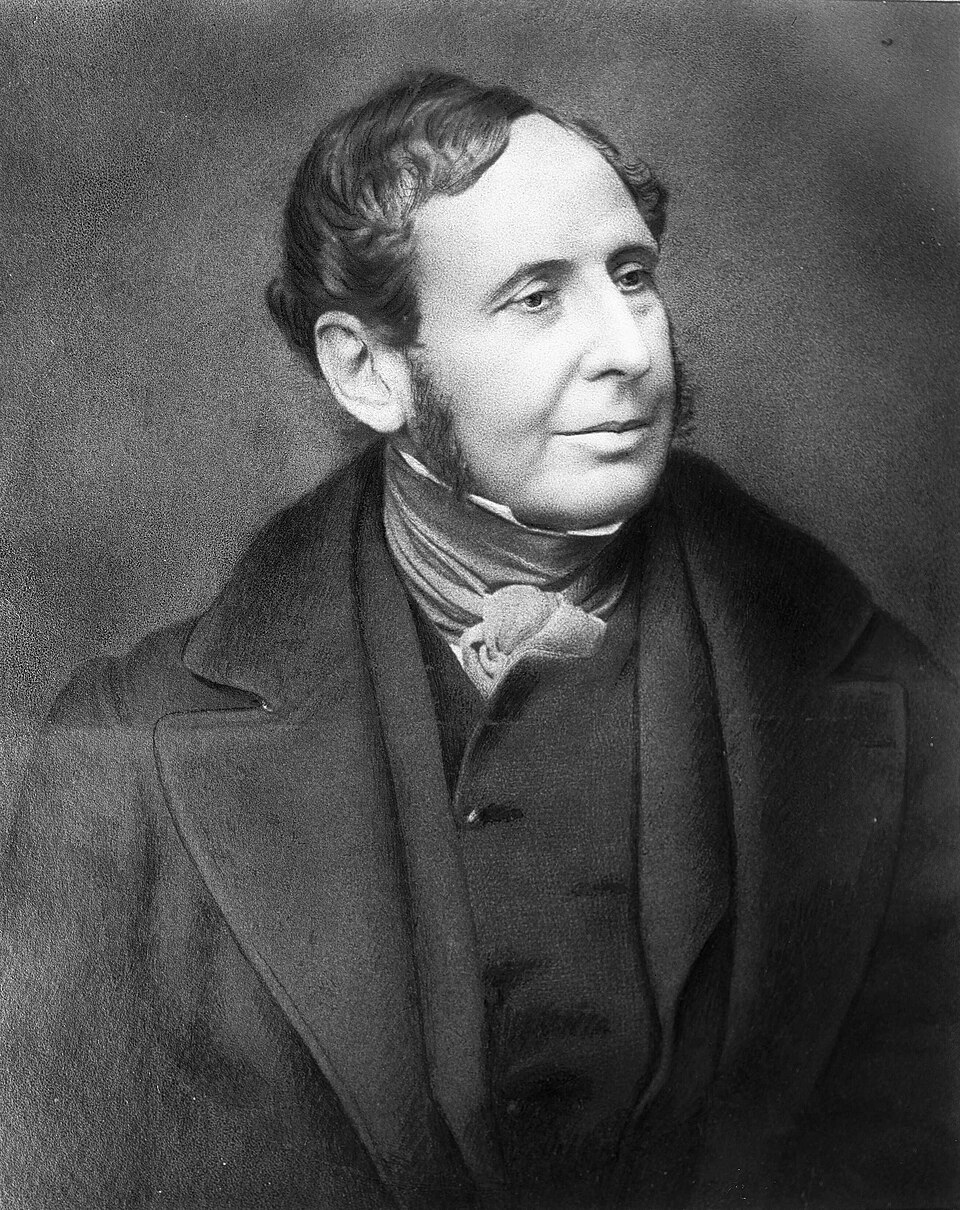
\includegraphics[height=0.27\textheight]{ch1_fitzroy_1910.jpg}\\[1mm]
\imgcap{Robert FitzRoy (1805--1865)}
\imgcredit{https://commons.wikimedia.org/wiki/File:Robert_Fitzroy.jpg}{Portrait: Charles Hemus (c.\ 1910); public domain; Wikimedia Commons}\\[1mm]\centering
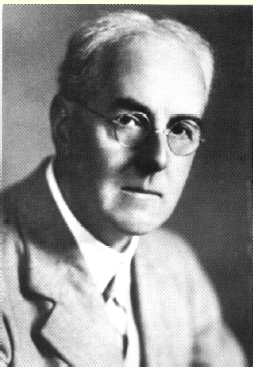
\includegraphics[height=0.22\textheight]{ch1_richardson.png}\\[1mm]
\imgcap{Lewis Fry Richardson (1881--1953)}
\imgcredit{https://commons.wikimedia.org/wiki/File:Lewis_Fry_Richardson.png}{Photo: NOAA; public domain; Wikimedia Commons}
\end{column}
\begin{column}{0.62\textwidth}
\begin{itemize}
    \item 1861: FitzRoy, head of the new Meteorological Office, publishes daily ``forecasts'' in The Times
    \begin{itemize}
        \item he coined the word in its modern sense; the forecasts were often wrong and publicly mocked
    \end{itemize}
    \item 1922: Richardson computes a weather forecast by numerical integration of the equations of motion, by hand
    \item 1950: \refBrier\ proposes a score for probability forecasts of rain; meteorology leads forecast verification for the next fifty years
    \begin{itemize}
        \item economics adopts the same tools late: PIT \refDGT, proper scores \refGRa, calibration \refGBR
    \end{itemize}
    \item Lesson: a forecast is only as useful as the way we evaluate it
\end{itemize}
\end{column}
\end{columns}
\end{frame}


%=============================================================================
\section{Point forecasts and loss functions}
%=============================================================================

\begin{frame}{Setting and notation}
\itemsize{\small}
\begin{itemize}
    \item Target $Y_{t+h}$, information set $\mathcal{F}_t$, horizon $h$; a \textbf{point forecast} $\hat y_{t+h|t}$ is $\mathcal{F}_t$-measurable
    \begin{itemize}
        \item $\mathcal{F}_t$-measurable: computed only from information available at $t$
        \item a \textbf{probabilistic forecast} is a predictive distribution $F_{t+h|t}$ (density, quantiles, interval, ensemble)
    \end{itemize}
    \item Out-of-sample design: $R$ observations to estimate, $P$ forecasts to evaluate, $R + P + h - 1 = T$
    \begin{itemize}
        \item schemes: \textbf{fixed} (estimate once), \textbf{rolling} (last $R$), \textbf{recursive} (all past); \atschlink{https://danpele.github.io/Time-Series-Analysis/EN/Courses/chapter4_seasonality_forecasting.pdf}{TSA, Chapter 4} called this rolling-origin evaluation
        \item $T$: the total sample; the last forecast, made at $R + P - 1$, targets $T$; the scheme matters for inference: \refWest\ versus \refGW, Section 4
    \end{itemize}
    \item Known from \atschlink{https://danpele.github.io/Time-Series-Analysis/EN/Courses/chapter0_introduction.pdf}{TSA, Chapter 0}: MAE, RMSE, MAPE and the scale-free MASE \refHK
    \begin{itemize}
        \item $\mathrm{MAE} = P^{-1}\sum|e_t|$, $\mathrm{RMSE} = (P^{-1}\sum e_t^2)^{1/2}$, $\mathrm{MAPE} = 100P^{-1}\sum|e_t/y_t|$; MASE: the MAE divided by the in-sample MAE of the naive forecast
        \item here the question is different: \emph{which} loss, and what does it reward?
    \end{itemize}
\end{itemize}
\end{frame}

\begin{frame}{The optimal point forecast and consistency (1/2)}
\itemsize{\small}
\begin{itemize}
    \item Given a loss $L(x, y)$ and a predictive distribution $F$, the \textbf{optimal} (Bayes) forecast minimises the expected loss:
    \begin{itemize}
        \item $x^* = \arg\min_x \E_F[L(x, Y)]$
        \item $x$: the point forecast; $y$: the outcome; $L(x, y) \ge 0$: the penalty; $\E_F$: the expectation when $Y \sim F$
    \end{itemize}
    \item A \textbf{functional} $\mathrm{T}(F)$ maps a distribution to a number: the mean, the median, a quantile
    \begin{itemize}
        \item $L$ is \textbf{consistent} for $\mathrm{T}$ if $\E_F L(\mathrm{T}(F), Y) \le \E_F L(x, Y)$ for all $x$ and $F$ \refGnaa
        \item i.e.\ reporting $\mathrm{T}(F)$ is optimal whatever $F$ is; \textbf{strictly} consistent: equality only at $x = \mathrm{T}(F)$
    \end{itemize}
\end{itemize}
\end{frame}

\begin{frame}{The optimal point forecast and consistency (2/2)}
\itemsize{\small}
\begin{itemize}
    \item Three classical cases, with the forecast error $e = y - x$; set the derivative of the expected loss to zero
    \begin{itemize}
        \item squared $e^2$: $\frac{d}{dx}\E(Y - x)^2 = -2\E(Y - x) = 0 \Rightarrow x^* = \E Y$ (the mean)
        \item absolute $|e|$: $\frac{d}{dx}\E|Y - x| = F(x) - (1 - F(x)) = 0 \Rightarrow F(x^*) = 1/2$ (the median)
        \item pinball $\rho_\tau(e) = (\tau - \mathbf 1\{e < 0\})e$: $F(x) - \tau = 0 \Rightarrow x^* = F^{-1}(\tau)$ (the $\tau$-quantile)
    \end{itemize}
    \item Notation of the pinball loss
    \begin{itemize}
        \item $\tau \in (0, 1)$: the quantile level; $\mathbf 1\{e < 0\}$: 1 if the forecast is too high, 0 otherwise; $F^{-1}$: the quantile function
        \item under-forecasts cost $\tau|e|$, over-forecasts $(1 - \tau)|e|$: a high $\tau$ pushes the forecast up
    \end{itemize}
    \item Consequence: announce the loss \emph{before} asking for a forecast; a median forecast judged by RMSE is judged unfairly \refGnaa
\end{itemize}
\end{frame}

\begin{frame}{Three losses, three optimal forecasts}
\itemsize{\footnotesize}
\begin{center}
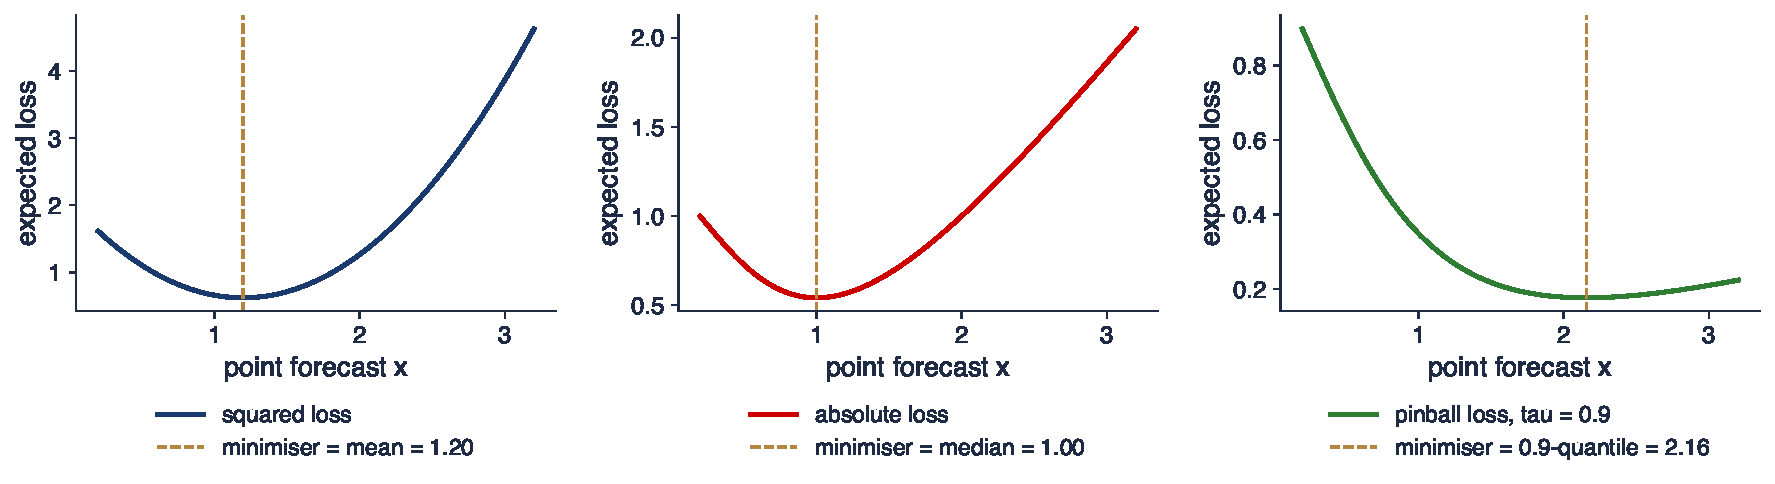
\includegraphics[width=0.97\textwidth,height=0.52\textheight,keepaspectratio]{ats_ch1_loss_minimizers.pdf}
\end{center}
\vspace{-0.25cm}
\begin{itemize}
    \item $Y$ log-normal with $\ln Y \sim N(0, 0.6^2)$; expected loss as a function of the point forecast $x$ (simulation, $2 \times 10^5$ draws)
\end{itemize}
\quantlet{ATS\_ch1\_loss\_functions}{\qlurl{ATS_ch1_loss_functions}}
\end{frame}

\begin{frame}{Interpreting the three minimisers}
\itemsize{\small}
\begin{itemize}
    \item Mean 1.20, median 1, 0.9-quantile 2.16; three different ``best'' forecasts of the same variable
    \begin{itemize}
        \item for a right-skewed target (wages, loads, prices, volatility) the gap is large
    \end{itemize}
    \item The pinball curve is flat near its minimum: quantile forecasts are hard to separate with few observations
    \item A forecaster who knows the loss reports the matching functional; ranking forecasts by another loss rewards the wrong behaviour
\end{itemize}
\end{frame}

\begin{frame}{Bregman losses: all losses consistent for the mean (1/2)}
\itemsize{\small}
\begin{itemize}
    \item \textbf{Theorem} \refSav, \refGnaa: under regularity, $L$ is consistent for the mean iff it is a \textbf{Bregman} loss
    \begin{itemize}
        \item $L(x, y) = \phi(y) - \phi(x) - \phi'(x)(y - x)$
        \item $\phi$: a convex function, $\phi'$ its derivative; $L$ is the gap between $\phi(y)$ and the tangent of $\phi$ at $x$, so $L \ge 0$ (up to terms in $y$ only)
    \end{itemize}
    \item Two members of the family
    \begin{itemize}
        \item $\phi(x) = x^2$: the squared error $(y - x)^2$
        \item $\phi(x) = -\ln x$: \textbf{QLIKE} $y/x - \ln(y/x) - 1$, for a variance forecast $x > 0$ and a variance proxy $y > 0$ (\atschlink{https://danpele.github.io/Advanced-Time-Series/EN/Courses/chapter8_advanced_volatility.pdf}{Chapter 8})
        \item the conditional mean is optimal for every Bregman loss \refBGW; proof for the quantile in the \atsapplink{atsapp1}{atssrc1}{Appendix}
    \end{itemize}
\end{itemize}
\end{frame}

\begin{frame}{Bregman losses: all losses consistent for the mean (2/2)}
\itemsize{\small}
\begin{itemize}
    \item Proof sketch, with $\mu = \E Y$:
    \begin{itemize}
        \item $\E L(x, Y) - \E L(\mu, Y) = \phi(\mu) - \phi(x) - \phi'(x)(\mu - x) \ge 0$
        \item the linear term vanishes because $\E(Y - \mu) = 0$; the inequality is convexity of $\phi$
    \end{itemize}
    \item Correctly specified forecasts rank the same under every Bregman loss; misspecified ones need not \refPatbz
    \begin{itemize}
        \item Murphy diagrams \refEGJK\ plot the score over the whole family: one forecast dominates only if its curve is lower everywhere
        \item robust proxies for volatility: only some losses keep the ranking with a noisy proxy \refPataa
    \end{itemize}
\end{itemize}
\end{frame}

\begin{frame}{Asymmetric loss}
\itemsize{\small}
\begin{itemize}
    \item \textbf{LinEx} loss $L(e) = b[\exp(ae) - ae - 1]$, $e = y - x$: linear on one side, exponential on the other
    \begin{itemize}
        \item $b > 0$: a scale; $a$: the asymmetry; $a > 0$ penalises under-forecasts ($e > 0$) exponentially, over-forecasts about linearly
        \item optimal forecast $x^* = a^{-1}\ln\E e^{aY}$; with $Y \mid \mathcal F_t \sim N(\mu_t, \sigma_t^2)$ (conditional mean $\mu_t$, variance $\sigma_t^2$): $x^* = \mu_t + a\sigma^2_t/2$ \refCD
        \item the optimal forecast is \textbf{biased} and its bias moves with the conditional variance
    \end{itemize}
    \item Consequences for evaluation
    \begin{itemize}
        \item a rational forecaster under asymmetric loss fails the MZ unbiasedness test (Section 4)
        \item the pinball loss is the piecewise-linear member: the optimal forecast is a quantile
    \end{itemize}
    \item Examples: a grid operator (under-forecasting load is costlier than over-forecasting), a central bank with asymmetric inflation costs, the capital buffer of a bank (\atschlink{https://danpele.github.io/Advanced-Time-Series/EN/Courses/chapter9_var_es_backtesting.pdf}{Chapter 9})
\end{itemize}
\end{frame}

\begin{frame}{Recap: Point forecasts and loss functions}
\itemsize{\small}
\begin{itemize}
    \item A loss defines the target functional: squared $\to$ mean, absolute $\to$ median, pinball $\to$ quantile
    \item Bregman losses are exactly those consistent for the mean; QLIKE is one of them
    \item Under asymmetric loss the optimal forecast is biased by design
    \item With misspecified models the ranking can depend on the loss: fix it in advance
\end{itemize}
\end{frame}


%=============================================================================
\section{Probabilistic forecasts: calibration and sharpness}
%=============================================================================

\begin{frame}{Maximise sharpness subject to calibration}
\itemsize{\small}
\begin{itemize}
    \item \textbf{Calibration}: statistical consistency between the forecasts $F_t$ and the outcomes $y_t$ (a joint property) \refGBR
    \begin{itemize}
        \item \textbf{probabilistic} calibration: the PIT (probability integral transform) $u_t = F_t(y_t)$, the forecast probability of an outcome below $y_t$, is uniform on average
        \item \textbf{marginal} calibration: $\frac1T\sum_t F_t(x) \to G(x)$ for every $x$, with $G$ the limit of the empirical distribution of $y_t$
    \end{itemize}
    \item \textbf{Sharpness}: concentration of the predictive distributions; a property of the forecasts only
    \begin{itemize}
        \item measured by the average width of central intervals or the average predictive variance
    \end{itemize}
    \item Paradigm \refGBR: among calibrated forecasts, prefer the sharpest
    \begin{itemize}
        \item the climatological forecast (the unconditional distribution) is calibrated but not sharp
        \item proper scores (next section) reward both at once
    \end{itemize}
\end{itemize}
\end{frame}

\begin{frame}{The probability integral transform}
\itemsize{\small}
\begin{itemize}
    \item \textbf{Theorem} \refDawid, \refDGT: if $F_t$ is the true conditional distribution of $Y_t$ given $\mathcal{F}_{t-1}$ and continuous, then $u_t = F_t(y_t)$ are i.i.d.\ $U(0, 1)$
    \begin{itemize}
        \item uniform: for every $v \in (0,1)$, $P(u_t \le v \mid \mathcal{F}_{t-1}) = P(Y_t \le F_t^{-1}(v) \mid \mathcal F_{t-1}) = v$, whatever the past
        \item independent: a conditional distribution that does not depend on the past implies independence of the sequence
    \end{itemize}
    \item For $h > 1$ the PITs are uniform but serially dependent up to lag $h - 1$ (overlapping horizons)
    \begin{itemize}
        \item tests must allow this dependence \refRS
    \end{itemize}
    \item Uniformity is necessary, not sufficient: \refHamill\ and \refGBR\ build uncalibrated forecasters whose PIT is uniform on average
    \begin{itemize}
        \item check PIT conditionally: by sub-sample, by regime, by horizon
    \end{itemize}
\end{itemize}
\end{frame}

\begin{frame}{PIT histogram shapes}
\itemsize{\footnotesize}
\begin{center}
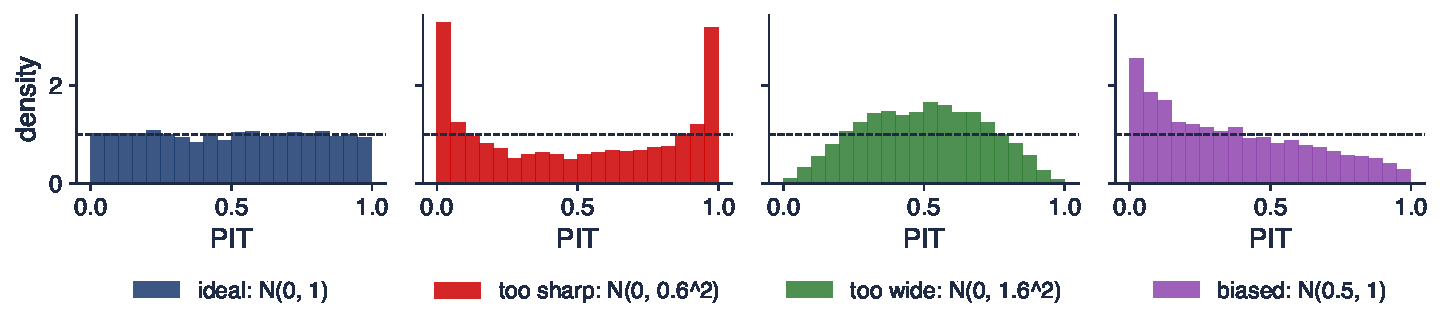
\includegraphics[width=0.97\textwidth,height=0.48\textheight,keepaspectratio]{ats_ch1_pit_shapes.pdf}
\end{center}
\vspace{-0.25cm}
\begin{itemize}
    \item $Y \sim N(0, 1)$, 5000 draws; four Normal forecasts; dashed line: the uniform density
\end{itemize}
\quantlet{ATS\_ch1\_calibration\_scores}{\qlurl{ATS_ch1_calibration_scores}}
\end{frame}

\begin{frame}{Interpreting the PIT shapes}
\itemsize{\small}
\begin{itemize}
    \item \textbf{U-shape}: too many outcomes in both tails (32\% outside the central 90\%, against 10\%): the forecast is too sharp, intervals too narrow
    \item \textbf{Hump}: too few outcomes in the tails (1.0\%): the forecast is too wide, the intervals waste information
    \item \textbf{Slope}: a biased location; here the forecast mean is too high, so PIT values cluster near 0
    \item CRPS (lower is better): ideal 0.567, too sharp 0.595, too wide 0.604, biased 0.637: the proper score ranks the ideal forecast first
\end{itemize}
\end{frame}

\begin{frame}{Testing calibration (1/2)}
\itemsize{\small}
\begin{itemize}
    \item \textbf{Berkowitz test} \refBerk: if the PITs are i.i.d.\ uniform, $z_t = \Phi^{-1}(u_t)$ is i.i.d.\ $N(0, 1)$
    \begin{itemize}
        \item $\Phi^{-1}$: the quantile function of the standard Normal distribution
    \end{itemize}
    \item Fit a Gaussian AR(1) to $z_t$ and test its parameters:
    \begin{itemize}
        \item $z_t = \mu + \rho(z_{t-1} - \mu) + \varepsilon_t$, $\quad \varepsilon_t \sim N(0, \sigma^2(1 - \rho^2))$
        \item $\mu$: the mean of $z_t$; $\sigma^2$: its variance; $\rho$: its first-order autocorrelation; calibration means $\mu = 0$, $\sigma = 1$, $\rho = 0$
        \item LR (likelihood ratio) statistic $2(\ell_1 - \ell_0) \sim \chi^2(3)$ under $H_0$; $\ell_1, \ell_0$: maximised log-likelihoods without and with the restrictions
        \item the transformation to $z$ makes the tails visible; the test checks only the first two moments and AR(1) dependence
    \end{itemize}
\end{itemize}
\end{frame}

\begin{frame}{Testing calibration (2/2)}
\itemsize{\small}
\begin{itemize}
    \item \textbf{Correlograms} of $(u_t - \bar u)^k$, $k = 1, 2$ \refDGT: dependence in level and in volatility
    \begin{itemize}
        \item $\bar u$: the mean PIT; Ljung--Box on $(u_t - \bar u)^2$ detects missing volatility dynamics
    \end{itemize}
    \item Parameter estimation changes the null distribution of PIT tests
    \begin{itemize}
        \item with $P/R$ small (few forecasts relative to the estimation sample) it can be ignored, otherwise use \refRS
    \end{itemize}
    \item Interval forecasts: coverage and independence of the hits \refChr
    \begin{itemize}
        \item hit: an outcome outside the interval; for VaR this becomes backtesting (\atschlink{https://danpele.github.io/Advanced-Time-Series/EN/Courses/chapter9_var_es_backtesting.pdf}{Chapter 9})
    \end{itemize}
\end{itemize}
\end{frame}

\begin{frame}{Case study: Diebold, Gunther and Tay (1998)}
\itemsize{\small}
\begin{itemize}
    \item The paper: daily S\&P 500 returns; parameters estimated once on the first part of the sample, density forecasts evaluated on the second part with PIT histograms and correlograms of $(u - \bar u)^k$ \refDGT
    \begin{itemize}
        \item their models: i.i.d.\ Normal; MA(1)-GARCH(1,1) with Normal and with Student-$t$ innovations \refBoll
    \end{itemize}
    \item Our replication: the same three models, estimated by maximum likelihood on 2000--2012, fixed parameters, one-day density forecasts for 2013--2026 ($3\,448$ days)
    \begin{itemize}
        \item model: $r_t = c + \varepsilon_t + \theta\varepsilon_{t-1}$, $\varepsilon_t = \sigma_tz_t$, $\sigma_t^2 = \omega + \alpha\varepsilon_{t-1}^2 + \beta\sigma_{t-1}^2$; $z_t$ Normal or Student-$t$ with $\nu$ degrees of freedom
        \item GARCH-$t$: $\hat\theta = \ensuremath{-}0.061$, $\hat\alpha + \hat\beta = 0.996$ (the persistence of volatility), $\hat\nu = 8.0$ (fat tails)
    \end{itemize}
    \item Question: which density forecast is calibrated, and do the proper scores agree with the PIT diagnosis?
\end{itemize}
\end{frame}

\begin{frame}{PIT diagnostics of three S\&P 500 density forecasts}
\itemsize{\footnotesize}
\begin{center}
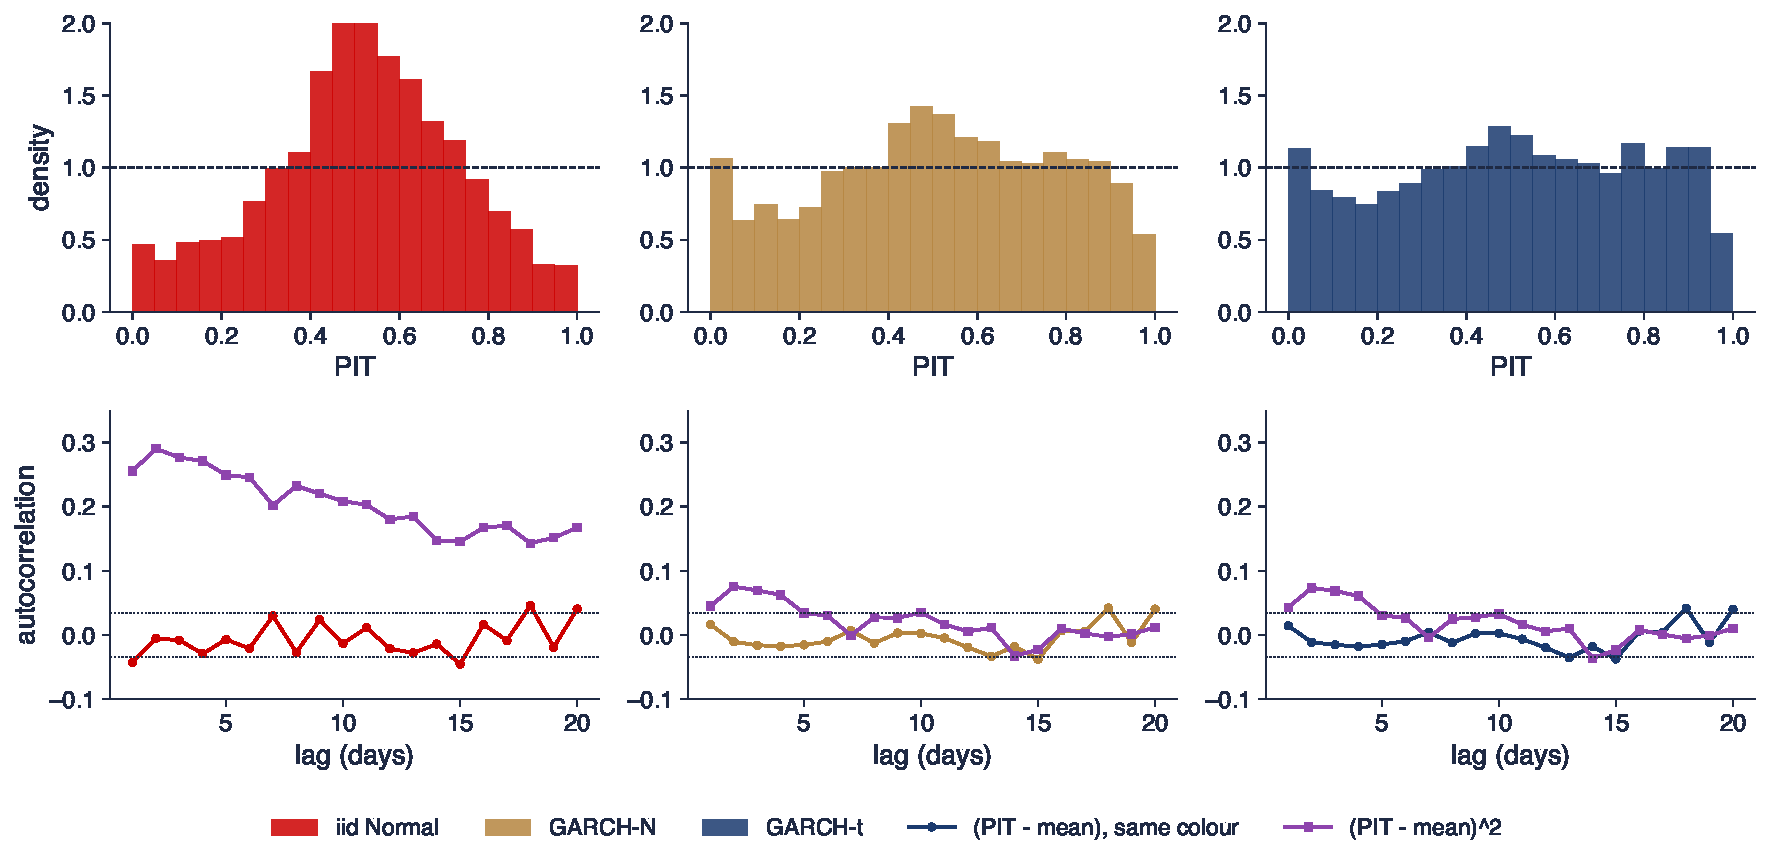
\includegraphics[width=0.97\textwidth,height=0.68\textheight,keepaspectratio]{ats_ch1_dgt.pdf}
\end{center}
\vspace{-0.25cm}
\begin{itemize}
    \item Top: PIT histograms (20 bins); bottom: autocorrelations of $(u - \bar u)$ and $(u - \bar u)^2$ with $\pm 2/\sqrt{T}$ bands
\end{itemize}
\quantlet{ATS\_ch1\_density\_forecasts}{\qlurl{ATS_ch1_density_forecasts}}
\end{frame}

\begin{frame}{Interpreting the S\&P 500 diagnostics}
\itemsize{\small}
\begin{itemize}
    \item i.i.d.\ Normal: a hump and strong autocorrelation of $(u - \bar u)^2$: the forecast ignores volatility clustering; Berkowitz LR 428.8 ($p$ $<$\,0.001)
    \begin{itemize}
        \item too wide in calm periods, too narrow in turbulent ones: the two errors average into a hump
    \end{itemize}
    \item GARCH removes most of the dependence; the $t$ version has the better left tail
    \begin{itemize}
        \item Berkowitz: GARCH-N LR 9.3 ($p$ 0.026), GARCH-$t$ LR 10.0 ($p$ 0.019); estimated $\sigma_z$ 0.97 $< 1$
        \item with parameters frozen in 2012 the forecasts are slightly too wide after 2013: fewer than 10\% of days fall outside the central 90\% (scores table, next section)
    \end{itemize}
    \item In line with \refDGT: conditional heteroskedasticity is essential, fat tails help; a small residual miscalibration remains
\end{itemize}
\end{frame}

\begin{frame}{Recap: Calibration}
\itemsize{\small}
\begin{itemize}
    \item Calibration is a joint property of forecasts and outcomes; sharpness is a property of the forecasts
    \item Correct one-step densities give i.i.d.\ uniform PITs; for $h > 1$ they are dependent
    \item U-shape: too sharp; hump: too wide; slope: bias; correlogram of $(u - \bar u)^2$: missing volatility dynamics
    \item The S\&P 500: GARCH-$t$ is close to calibrated, the i.i.d.\ Normal is not
\end{itemize}
\end{frame}


%=============================================================================
\section{Proper scoring rules and elicitability}
%=============================================================================

\begin{frame}{Proper scoring rules}
\itemsize{\small}
\begin{itemize}
    \item A \textbf{scoring rule} $S(F, y)$ assigns a penalty to the forecast $F$ when $y$ occurs (negatively oriented: lower is better)
    \begin{itemize}
        \item \textbf{proper}: $\E_G S(G, Y) \le \E_G S(F, Y)$ for all $F, G$ \refGRa
        \item $G$: the distribution the forecaster believes; $\E_G$: the expectation under $G$; reporting the true belief is optimal
        \item \textbf{strictly proper}: equality only if $F = G$; then the score cannot be manipulated
    \end{itemize}
    \item Proper scores reward calibration and sharpness together: the expected score decomposes into uncertainty, minus resolution, plus reliability
    \begin{itemize}
        \item the Brier score $(p - \mathbf 1\{\text{event}\})^2$, with $p$ the forecast probability of a binary event, is the oldest example \refBrier
    \end{itemize}
    \item A proper score of a probabilistic forecast reduces to a consistent loss of a point forecast when $F$ is a point mass (example: the CRPS, two slides later)
\end{itemize}
\end{frame}

\begin{frame}{The logarithmic score}
\itemsize{\small}
\begin{itemize}
    \item $\mathrm{LogS}(f, y) = -\ln f(y)$ \refGood: the only proper score that is \textbf{local} (depends on $f$ only at $y$, up to equivalence)
    \begin{itemize}
        \item $f$: the forecast density; $g$: the true density; properness: $\E_g[\mathrm{LogS}(f, Y)] - \E_g[\mathrm{LogS}(g, Y)] = \int g \ln(g/f) = \mathrm{KL}(g \| f) \ge 0$
        \item $\mathrm{KL}$: the Kullback--Leibler divergence, nonnegative and zero only if $f = g$ (Gibbs inequality)
    \end{itemize}
    \item Links: average log score = minus the out-of-sample log-likelihood; the difference of two log scores is a predictive likelihood ratio
    \begin{itemize}
        \item Bayes factors and the predictive model choice of \refGA\ are built on it
    \end{itemize}
    \item Weaknesses: infinite if $f(y) = 0$; very sensitive to tail events; needs a density
    \begin{itemize}
        \item cannot score ensembles or quantile forecasts directly
    \end{itemize}
\end{itemize}
\end{frame}

\begin{frame}{The continuous ranked probability score (1/2)}
\itemsize{\small}
\begin{itemize}
    \item Definition \refMW: the squared distance between the forecast distribution function and the step function of the outcome
    \begin{itemize}
        \item $\mathrm{CRPS}(F, y) = \int_{-\infty}^{\infty}(F(z) - \mathbf 1\{y \le z\})^2dz$
        \item $z$: a threshold; $\mathbf 1\{y \le z\}$: the ``distribution function'' of the outcome, 0 below $y$ and 1 above; units: those of $y$
    \end{itemize}
    \item Kernel form \refGRa\ (proof in the \atsapplink{atsapp2}{atssrc2}{Appendix}):
    \begin{itemize}
        \item $\mathrm{CRPS}(F, y) = \E_F|X - y| - \frac12\E_F|X - X'|$, $\quad X, X' \sim F$ independent
        \item first term: accuracy; second: a reward for spread that stops the score from favouring point masses
        \item for a point forecast ($F$ a point mass at $x$) it reduces to the absolute error $|y - x|$
    \end{itemize}
\end{itemize}
\end{frame}

\begin{frame}{The continuous ranked probability score (2/2)}
\itemsize{\small}
\begin{itemize}
    \item Closed form for $F = N(\mu, \sigma^2)$, with $z = (y - \mu)/\sigma$:
    \begin{itemize}
        \item $\mathrm{CRPS} = \sigma\left[z(2\Phi(z) - 1) + 2\varphi(z) - 1/\sqrt\pi\right]$
        \item $\Phi$, $\varphi$: the distribution and density functions of $N(0,1)$; a closed form exists also for Student $t$ (Quantlet)
        \item ensembles: plug in the empirical distribution of the members
    \end{itemize}
    \item Decompositions:
    \begin{itemize}
        \item $\mathrm{CRPS} = \int \mathrm{BS}_z\,dz = 2\int_0^1 \rho_\tau(y - F^{-1}(\tau))\,d\tau$
        \item $\mathrm{BS}_z$: the Brier score of the event $\{y \le z\}$; $\rho_\tau$: the pinball loss at level $\tau$
        \item so the average pinball over the 99 percentiles (GEFCom2014) approximates CRPS/2 \refGEF
    \end{itemize}
\end{itemize}
\end{frame}

\begin{frame}{Quantile, interval and multivariate scores (1/2)}
\itemsize{\small}
\begin{itemize}
    \item \textbf{Quantile score}: $\rho_\tau(y - q)$ for a forecast $q$ of the $\tau$-quantile, strictly consistent \refGnaa
    \begin{itemize}
        \item any increasing $g$ gives another consistent score: $(\mathbf 1\{y \le q\} - \tau)(g(q) - g(y))$
    \end{itemize}
    \item \textbf{Interval score} of a central $(1 - \alpha)$ interval $[l, u]$ \refGRa
    \begin{itemize}
        \item $\mathrm{IS}_\alpha = (u - l) + \frac2\alpha(l - y)\mathbf 1\{y < l\} + \frac2\alpha(y - u)\mathbf 1\{y > u\}$
        \item $l, u$: the lower and upper limits; width plus a penalty $2/\alpha$ per unit of miss
        \item it equals $\frac2\alpha[\rho_{\alpha/2}(y - l) + \rho_{1 - \alpha/2}(y - u)]$; coverage alone is not a score
    \end{itemize}
\end{itemize}
\end{frame}

\begin{frame}{Quantile, interval and multivariate scores (2/2)}
\itemsize{\small}
\begin{itemize}
    \item \textbf{Energy score} for vectors, the multivariate CRPS:
    \begin{itemize}
        \item $\mathrm{ES}(F, \mathbf y) = \E\|\mathbf X - \mathbf y\| - \frac12\E\|\mathbf X - \mathbf X'\|$
        \item $\mathbf y$: the outcome vector; $\mathbf X, \mathbf X'$: independent draws from the forecast $F$; $\|\cdot\|$: the Euclidean norm
        \item weak at detecting wrong correlations; the \textbf{variogram score} \refSH\ targets the dependence structure (24 hourly loads, a VAR path)
        \item $\mathrm{VS}_p = \sum_{i,j}w_{ij}\big(|y_i - y_j|^p - \E|X_i - X_j|^p\big)^2$: compares observed and forecast differences between components; $w_{ij} \ge 0$: weights, $p$: usually 0.5
    \end{itemize}
    \item Tails: threshold-weighted CRPS stays proper \refGRjaa
    \begin{itemize}
        \item $\int (F(z) - \mathbf 1\{y \le z\})^2w(z)dz$
        \item $w(z) \ge 0$: a weight that emphasises the thresholds of interest (e.g.\ the left tail); the weighted likelihood ratio of \refAG\ does not stay proper \refGRjaa
    \end{itemize}
\end{itemize}
\end{frame}

\begin{frame}{Proper and improper scores}
\itemsize{\footnotesize}
\begin{center}
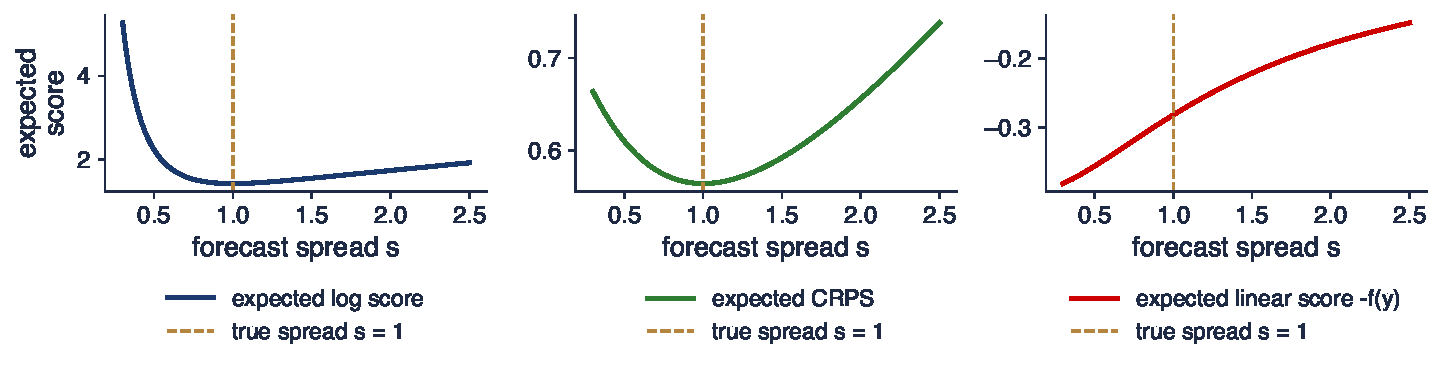
\includegraphics[width=0.97\textwidth,height=0.48\textheight,keepaspectratio]{ats_ch1_proper_scores.pdf}
\end{center}
\vspace{-0.25cm}
\begin{itemize}
    \item Truth $Y \sim N(0, 1)$; forecast $N(0, s^2)$; expected score as a function of the spread $s$ (closed forms)
    \item Log score and CRPS: minimum at $s = 1$; linear score $-f(y)$: $\E f(Y) = [2\pi(1 + s^2)]^{-1/2}$ grows as $s \to 0$: it rewards overconfidence
\end{itemize}
\quantlet{ATS\_ch1\_calibration\_scores}{\qlurl{ATS_ch1_calibration_scores}}
\end{frame}

\begin{frame}{Interpreting the expected scores}
\itemsize{\small}
\begin{itemize}
    \item The log score and the CRPS are minimised by the true spread: a forecaster maximises the expected reward by reporting what she believes
    \item The log score punishes overconfidence much more than excess spread (steep left branch); the CRPS is more symmetric and bounded by the absolute error
    \item The linear score is maximised by a point mass: it would reward a forecaster who always reports a spike, so it must not be used for evaluation
\end{itemize}
\end{frame}

\begin{frame}{Elicitability}
\itemsize{\small}
\begin{itemize}
    \item A functional $\mathrm T$ is \textbf{elicitable} if a strictly consistent loss exists for it \refGnaa
    \begin{itemize}
        \item mean, quantiles, expectiles, ratios of expectations: elicitable
        \item only elicitable functionals can be compared and ranked meaningfully with point forecasts
    \end{itemize}
    \item \textbf{Necessary condition} (Osband): convex level sets: $\mathrm T(F_0) = \mathrm T(F_1) = t \Rightarrow \mathrm T(\lambda F_0 + (1 - \lambda)F_1) = t$
    \begin{itemize}
        \item $F_0, F_1$: two distributions with the same value $t$; $\lambda \in [0,1]$: the mixing weight
        \item the \textbf{variance} fails it, so it is not elicitable; the pair (mean, second moment) is
    \end{itemize}
    \item Risk measures with $\mathrm{VaR}_\alpha(X) = -q_\alpha(X)$, $q_\alpha$ the $\alpha$-quantile of the return $X$ (VaR 1\%: $\alpha = 0.01$)
    \begin{itemize}
        \item VaR is a quantile: elicitable by the pinball loss
        \item ES (expected shortfall, the mean loss beyond VaR) has non-convex level sets: \textbf{not elicitable} alone \refWeber, \refGnaa; (VaR, ES) is \textbf{jointly} elicitable \refFZ
        \item the Fissler--Ziegel scores and the backtests built on them: \atschlink{https://danpele.github.io/Advanced-Time-Series/EN/Courses/chapter9_var_es_backtesting.pdf}{Chapter 9}
    \end{itemize}
\end{itemize}
\end{frame}

\begin{frame}{Scores of the S\&P 500 density forecasts}
\itemsize{\footnotesize}
\begin{center}
\footnotesize
\begin{tabular}{lrrrr}
\toprule
\textbf{Model} & \textbf{Log score} & \textbf{CRPS} & \textbf{Outside 90\%} & \textbf{Berkowitz $p$} \\
\midrule
i.i.d.\ Normal & 1.531 & 0.564 & 3.9\% & $<$\,0.001 \\
MA(1)-GARCH(1,1)-N & 1.265 & 0.509 & 8.0\% & 0.026 \\
MA(1)-GARCH(1,1)-$t$ & 1.233 & 0.507 & 8.4\% & 0.019 \\
\bottomrule
\end{tabular}
\end{center}
\begin{itemize}
    \item Score differences tested with DM on the daily scores (\refAG, unweighted)
    \begin{itemize}
        \item GARCH-$t$ against GARCH-N: HLN \ensuremath{-}5.9 (log score), \ensuremath{-}6.4 (CRPS); GARCH-N against i.i.d.: \ensuremath{-}12.7 and \ensuremath{-}21.5
    \end{itemize}
    \item Both scores rank the models in the same order as the PIT diagnosis; the log score separates the tails more sharply
    \item Ranking and calibration are different questions: the best-scoring model can still fail a calibration test
\end{itemize}
\end{frame}

\begin{frame}{Recap: Proper scores and elicitability}
\itemsize{\small}
\begin{itemize}
    \item Proper scores make honesty optimal; strictly proper scores cannot be gamed
    \item LogS: local, tail-sensitive; CRPS: robust, works for ensembles, equals twice the integrated pinball loss
    \item Interval score for intervals, energy and variogram scores for vectors
    \item Elicitable: mean, quantile (VaR); not elicitable: variance, ES alone; (VaR, ES) jointly
\end{itemize}
\end{frame}


%=============================================================================
\section{Comparing forecasts}
%=============================================================================

\begin{frame}{Two questions about predictive ability}
\itemsize{\small}
\begin{itemize}
    \item \textbf{Population} \refWest: are the \emph{models}, at their pseudo-true parameters, equally accurate?
    \begin{itemize}
        \item estimation error enters the asymptotic variance unless $P/R \to 0$ or the loss is the one used in estimation
    \end{itemize}
    \item \textbf{Finite sample} \refGW: are the \emph{forecasting methods}, with their estimation windows, equally accurate?
    \begin{itemize}
        \item rolling window of fixed size $R$: estimation noise is part of the method; nested models allowed
    \end{itemize}
    \item \textbf{Diebold--Mariano} \refDM\ treats the forecasts as given (``primitives''): it compares forecasts, not models \refDie
    \begin{itemize}
        \item using DM to compare models with estimated parameters needs the West or GW framework
    \end{itemize}
\end{itemize}
\end{frame}

\begin{frame}{The Diebold--Mariano test with HAC variance (1/2)}
\itemsize{\small}
\begin{itemize}
    \item Loss differential $d_t = L(e_{1t}) - L(e_{2t})$; $H_0$: $\E d_t = 0$ (equal accuracy)
    \begin{itemize}
        \item $e_{it}$: the error of forecast $i$ at $t$; $d_t > 0$: forecast 2 did better at $t$; $d_t$ assumed covariance stationary
    \end{itemize}
    \item The statistic: the mean differential over its HAC standard error
    \begin{itemize}
        \item $\mathrm{DM} = \bar d/\sqrt{\hat\sigma^2_{LR}/P} \to N(0, 1)$, $\quad \sigma^2_{LR} = \gamma_0 + 2\sum_{k \ge 1}\gamma_k$
        \item $\bar d$: the mean of $d_t$ over the $P$ forecasts; $\gamma_k$: the autocovariances of $d_t$; $\sigma^2_{LR}$: its long-run variance (\atschlink{https://danpele.github.io/Advanced-Time-Series/EN/Courses/chapter0_refresher_inference.pdf}{Chapter 0})
        \item a large positive DM: forecast 2 is more accurate; reject at 5\% if $|\mathrm{DM}| > 1.96$
    \end{itemize}
\end{itemize}
\end{frame}

\begin{frame}{The Diebold--Mariano test with HAC variance (2/2)}
\itemsize{\small}
\begin{itemize}
    \item Optimal $h$-step errors are at most MA($h - 1$), so DM truncate at $h - 1$ lags with a \textbf{rectangular} kernel
    \begin{itemize}
        \item the rectangular estimate can be \textbf{negative}; Newey--West (Bartlett) weights keep it positive \refNW, at the cost of downward bias
        \item suboptimal forecasts have errors with longer memory: use a data-driven bandwidth (\atschlink{https://danpele.github.io/Advanced-Time-Series/EN/Courses/chapter0_refresher_inference.pdf}{Chapter 0})
    \end{itemize}
    \item \textbf{HLN correction} \refHLNig: a small-sample rescaling of DM
    \begin{itemize}
        \item $\mathrm{DM}^* = \mathrm{DM}\sqrt{(P + 1 - 2h + h(h - 1)/P)/P}$, compared with $t_{P-1}$
        \item the factor (below 1) removes the bias of the variance estimator for MA($h - 1$) errors; $t_{P-1}$: Student $t$ with $P - 1$ degrees of freedom, for small $P$
    \end{itemize}
\end{itemize}
\end{frame}

\begin{frame}{Size of DM and HLN in small samples}
\itemsize{\footnotesize}
\begin{center}
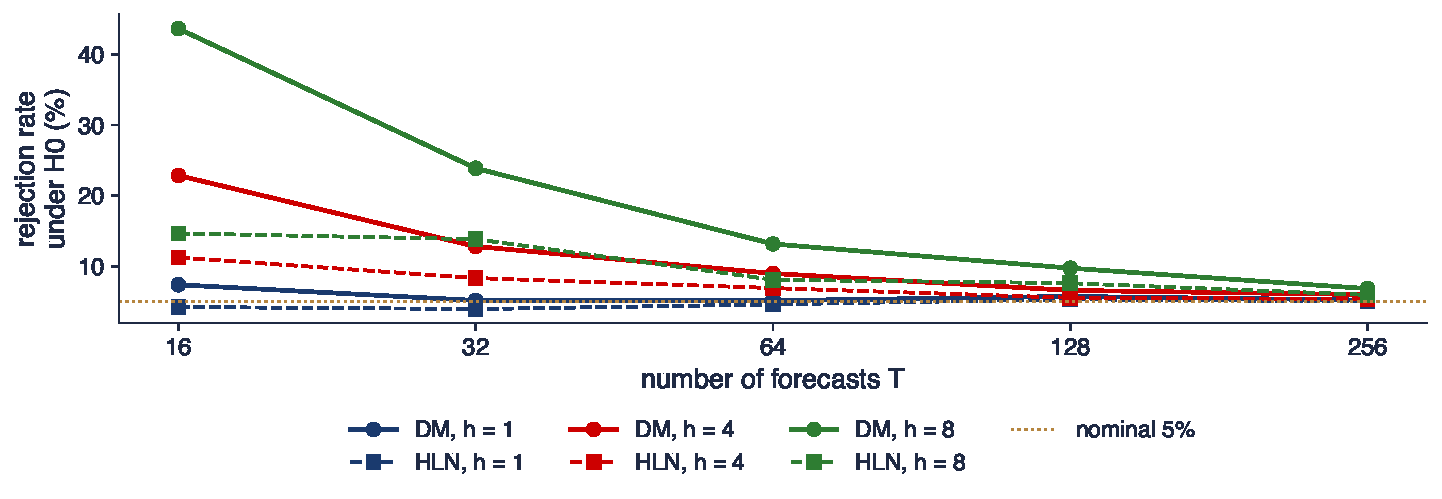
\includegraphics[width=0.97\textwidth,height=0.64\textheight,keepaspectratio]{ats_ch1_dm_size.pdf}
\end{center}
\vspace{-0.25cm}
\begin{itemize}
    \item Two independent MA($h - 1$) error series with equal variance, squared loss; share of rejections at 5\% in 4\,000 replications
\end{itemize}
\quantlet{ATS\_ch1\_dm\_tests}{\qlurl{ATS_ch1_dm_tests}}
\end{frame}

\begin{frame}{Interpreting the size experiment}
\itemsize{\small}
\begin{itemize}
    \item $h = 1$: both tests are close to 5\%; DM over-rejects only at $P = 16$ (7.4\%)
    \item $h = 8$, $P = 16$: DM rejects a true null 43.6\% of the time, HLN 14.6\%; at $P = 64$: 13.2\% and 8.1\%
    \begin{itemize}
        \item the HAC variance with few observations and many lags is noisy and biased down
    \end{itemize}
    \item Rule: at multi-step horizons with fewer than about 100 forecasts, use HLN and treat $p$-values near 5\% as inconclusive; fixed-$b$ critical values (\atschlink{https://danpele.github.io/Advanced-Time-Series/EN/Courses/chapter0_refresher_inference.pdf}{Chapter 0}) are an alternative
\end{itemize}
\end{frame}

\begin{frame}{Romanian inflation one year ahead: the design}
\itemsize{\small}
\begin{itemize}
    \item Target: HICP inflation, y/y, 12 months ahead; forecast origins from January 2013, targets January 2014 to August 2026, $P = 152$ forecasts
    \begin{itemize}
        \item HICP inflation in August 2026: 6.3\%
    \end{itemize}
    \item Forecasts
    \begin{itemize}
        \item \textbf{no change}: $\hat\pi_{t+12} = \pi_t$; \textbf{direct AR(3)}: $\pi_{t+12}$ on $1, \pi_t, \pi_{t-1}, \pi_{t-2}$, OLS on a 10-year rolling window
        \item \textbf{target}: the BNR inflation target, 2.5\%; \textbf{average} of AR(3) and no change
    \end{itemize}
    \item Overlapping 12-month targets: errors are serially correlated up to lag 11; DM with $h = 12$
\end{itemize}
\end{frame}

\begin{frame}{Romanian inflation forecasts one year ahead}
\itemsize{\footnotesize}
\begin{center}
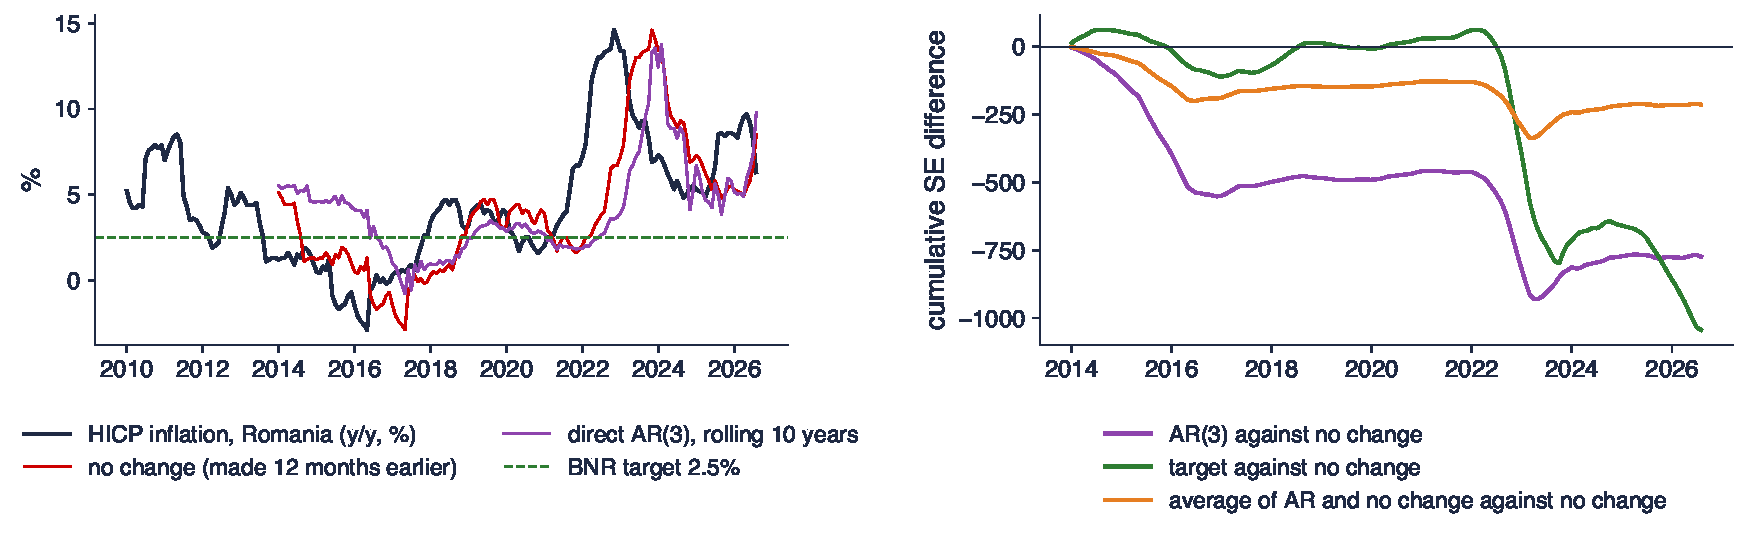
\includegraphics[width=0.97\textwidth,height=0.57\textheight,keepaspectratio]{ats_ch1_ro_inflation.pdf}
\end{center}
\vspace{-0.25cm}
\begin{itemize}
    \item Left: inflation and the forecasts made 12 months earlier; right: cumulative sum of $e_{\mathrm{nc},t}^2 - e_{m,t}^2$ (falling: model $m$ loses to no change)
\end{itemize}
\quantlet{ATS\_ch1\_dm\_tests}{\qlurl{ATS_ch1_dm_tests}}
\end{frame}

\begin{frame}{Interpreting the Romanian inflation comparison}
\itemsize{\footnotesize}
\begin{center}
\footnotesize
\begin{tabular}{lrrrrr}
\toprule
\textbf{Forecast} & \textbf{RMSE} & \textbf{DM} & \textbf{HLN} & \textbf{$p$ (HLN)} & \textbf{$p$, abs.\ loss} \\
\midrule
no change & 3.57 & -- & -- & -- & -- \\
AR(3) & 4.23 & 1.43 & 1.32 & 0.188 & 0.381 \\
BNR target & 4.43 & 1.30 & 1.21 & 0.230 & 0.319 \\
average & 3.76 & 0.96 & 0.88 & 0.378 & 0.795 \\
\bottomrule
\end{tabular}
\end{center}
\begin{itemize}
    \item Every model has a higher RMSE than no change, yet no difference is significant: with $P = 152$ overlapping targets the effective sample is small
    \item Newey--West instead of the rectangular kernel: HLN 1.47 for AR(3); the conclusion does not depend on the kernel
    \item Relative RMSE of AR(3): 1.44 before July 2021, 1.10 after: the ranking is not stable over time \refGRaz
\end{itemize}
\end{frame}

\begin{frame}{Conditional predictive ability: Giacomini--White (1/2)}
\itemsize{\small}
\begin{itemize}
    \item $H_0$: $\E[d_{t+h} \mid \mathcal{G}_t] = 0$ \refGW
    \begin{itemize}
        \item $\mathcal{G}_t$: the information at the forecast origin; $H_0$: no instrument $h_t \in \mathcal{G}_t$ predicts which method wins
        \item $h_t$: a $q \times 1$ vector of instruments (not the horizon $h$), e.g.\ a constant and the last loss differential
    \end{itemize}
    \item The statistic: a Wald test that the instruments do not predict $d_{t+h}$
    \begin{itemize}
        \item $\mathrm{GW} = P\,\bar Z'\hat\Omega^{-1}\bar Z \to \chi^2(q)$, $\quad Z_t = h_t d_{t+h}$
        \item $\bar Z$: the mean of $Z_t$; $\hat\Omega$: its HAC covariance matrix with $h - 1$ lags; $\chi^2(q)$: chi-squared with $q$ degrees of freedom
        \item $h_t = 1$ gives the unconditional test; adding $d_t$ or a state variable tests whether the past predicts the winner
    \end{itemize}
\end{itemize}
\end{frame}

\begin{frame}{Conditional predictive ability: Giacomini--White (2/2)}
\itemsize{\small}
\begin{itemize}
    \item Valid with a \textbf{rolling} window of fixed size, nested or non-nested models, any loss; invalid with a recursive window
    \begin{itemize}
        \item a rejection suggests a decision rule: use model 1 when $\hat\delta'h_t > 0$, with $\hat\delta$ the regression of $d_{t+h}$ on $h_t$
    \end{itemize}
    \item Romanian inflation, AR(3) against no change, $h_t = (1, d_t, \pi_t - 2.5)$
    \begin{itemize}
        \item $\pi_t - 2.5$: the distance of inflation from the BNR target
        \item $\mathrm{GW} = 3.19$, $p$ 0.363: neither the recent loss nor the distance from the target predicts the winner
    \end{itemize}
\end{itemize}
\end{frame}

\begin{frame}{Nested models: the failure of DM and the Clark--West test (1/2)}
\itemsize{\small}
\begin{itemize}
    \item Model 1 (small, e.g.\ the random walk) is nested in model 2; under $H_0$ the extra coefficients are zero
    \begin{itemize}
        \item MSPE: the mean squared prediction error; population MSPEs are equal, and $d_t$ is degenerate
        \item so the DM statistic is not asymptotically Normal \refCM
    \end{itemize}
    \item In finite samples model 2 estimates zero coefficients with noise
    \begin{itemize}
        \item its MSPE is \textbf{larger} than that of model 1: DM is undersized (rejects too rarely) and has little power
    \end{itemize}
\end{itemize}
\end{frame}

\begin{frame}{Nested models: the failure of DM and the Clark--West test (2/2)}
\itemsize{\small}
\begin{itemize}
    \item \textbf{Clark--West} \refCW: adjust the larger model for the noise it adds
    \begin{itemize}
        \item $f_t = e_{1t}^2 - [e_{2t}^2 - (\hat y_{1t} - \hat y_{2t})^2]$
        \item $e_{1t}, e_{2t}$: the errors of the small and large model; $\hat y_{1t}, \hat y_{2t}$: their forecasts; the squared gap between forecasts is the noise added by model 2
        \item one-sided $t$ test of $\E f_t = 0$ against $\E f_t > 0$ (model 2 better) with Normal critical values
    \end{itemize}
    \item Why the adjustment works
    \begin{itemize}
        \item under $H_0$, $\E e_1^2 - \E e_2^2 = -\E(\hat y_1 - \hat y_2)^2$: the adjustment recentres the differential (\atsapplink{atsapp3}{atssrc3}{Appendix})
        \item approximately Normal for rolling and recursive schemes; the exact critical values of \refCM\ are non-standard
    \end{itemize}
\end{itemize}
\end{frame}

\begin{frame}{Case study: Meese and Rogoff on EUR/RON}
\itemsize{\small}
\begin{itemize}
    \item \refMR: structural exchange-rate models do not beat the random walk out of sample at horizons up to one year
    \begin{itemize}
        \item their design: rolling out-of-sample forecasts, RMSE against the random walk; the result has survived forty years
    \end{itemize}
    \item Our data: monthly EUR/RON (BNR reference rate, end of month), $\Delta s_{t+1} = 100\Delta\ln S_{t+1}$; recursive estimation, forecasts January 2010 to August 2026 ($P = 200$)
    \begin{itemize}
        \item $S_t$: the rate (lei per euro); $\Delta s_{t+1}$: its monthly log change in \%, positive when the leu depreciates
        \item nested in the random walk ($\Delta\hat s = 0$): drift, AR($p$), the UIP regression $\Delta s_{t+1} = a + b(i^{RO}_t - i^{EA}_t)/12 + u$ \refFama
        \item $i^{RO}_t, i^{EA}_t$: 3-month interest rates in \% a year (divided by 12: per month); $a, b$: regression coefficients
        \item no estimated parameters: UIP imposed ($a = 0, b = 1$), momentum (mean of the last three changes)
    \end{itemize}
    \item UIP: uncovered interest parity, the expected depreciation equals the interest differential
\end{itemize}
\end{frame}

\begin{frame}{EUR/RON: models against the random walk}
\itemsize{\footnotesize}
\begin{center}
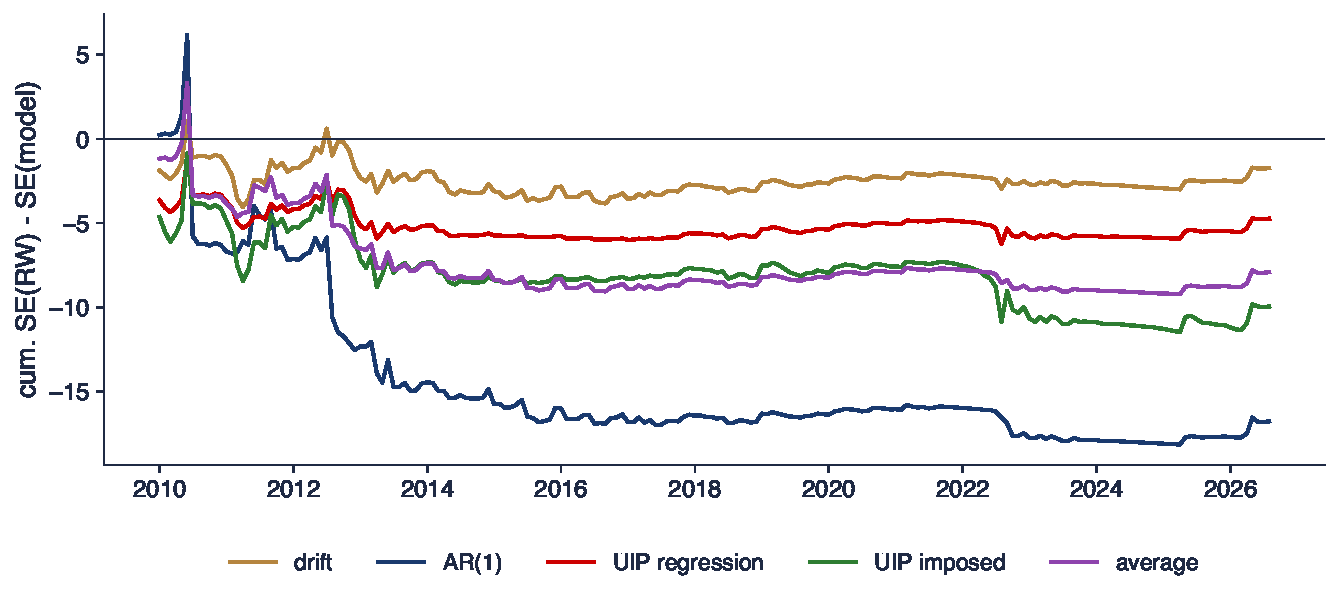
\includegraphics[width=0.97\textwidth,height=0.65\textheight,keepaspectratio]{ats_ch1_eurron.pdf}
\end{center}
\vspace{-0.25cm}
\begin{itemize}
    \item Cumulative $\sum_t(e^2_{RW,t} - e^2_{m,t})$ \refGWel: a line below zero means model $m$ has accumulated more squared error than the random walk
\end{itemize}
\quantlet{ATS\_ch1\_nested\_spa}{\qlurl{ATS_ch1_nested_spa}}
\end{frame}

\begin{frame}{Interpreting the EUR/RON tests}
\itemsize{\footnotesize}
\begin{center}
\scriptsize
\begin{tabular}{lrrrr}
\toprule
\textbf{Model} & \textbf{RMSE / RW} & \textbf{DM (HLN)} & \textbf{CW} & \textbf{$p$ (CW, one-sided)} \\
\midrule
drift & 1.006 & 0.27 & 1.06 & 0.145 \\
AR(1) & 1.055 & 1.13 & \ensuremath{-}0.15 & 0.561 \\
AR(4) & 1.062 & 1.29 & \ensuremath{-}0.43 & 0.666 \\
UIP regression & 1.016 & 0.76 & 0.10 & 0.458 \\
UIP imposed & 1.033 & 0.99 & -- & -- \\
momentum & 1.183 & 2.61 & -- & -- \\
average & 1.026 & 0.85 & -- & -- \\
\bottomrule
\end{tabular}
\end{center}
\begin{itemize}
    \item Every model has a higher RMSE than the random walk (random-walk RMSE 0.86 pp a month); the Meese--Rogoff result holds for the leu
    \item Clark--West does not reject either: the adjustment is not enough to make AR or UIP useful; only the drift gets close
    \item Managed float: the BNR smooths EUR/RON, so monthly changes are small and close to unpredictable from these predictors
\end{itemize}
\end{frame}

\begin{frame}{Rationality: Mincer--Zarnowitz and encompassing (1/2)}
\itemsize{\small}
\begin{itemize}
    \item \textbf{Mincer--Zarnowitz} \refMZ: regress the outcome on the forecast
    \begin{itemize}
        \item $y_{t+h} = a + b\hat y_{t+h|t} + u_{t+h}$
        \item under squared loss an optimal forecast has $(a, b) = (0, 1)$: no bias, and a one-unit forecast change predicts a one-unit outcome change
        \item Wald test of $(a, b) = (0, 1)$ with HAC errors ($u$ is MA($h - 1$)); $b < 1$: forecasts too volatile; $b > 1$: too timid
        \item extended version: add variables in $\mathcal{F}_t$; a significant coefficient means unused information
    \end{itemize}
    \item MZ assumes squared loss: under asymmetric loss a rational forecast is biased (Section 1)
\end{itemize}
\end{frame}

\begin{frame}{Rationality: Mincer--Zarnowitz and encompassing (2/2)}
\itemsize{\small}
\begin{itemize}
    \item \textbf{Encompassing} \refChH, \refHLNih: forecast 1 encompasses forecast 2 if 2 adds nothing to 1
    \begin{itemize}
        \item $y = (1 - \lambda)\hat y_1 + \lambda\hat y_2 + \varepsilon$, $\quad H_0$: $\lambda = 0$
        \item $\lambda$: the weight of forecast 2 in the best combination; $\lambda = 0$: forecast 2 is useless given forecast 1
        \item HLN test: DM--HLN on $d_t = e_{1t}(e_{1t} - e_{2t})$, one-sided ($\E d_t > 0$ means $\lambda > 0$)
    \end{itemize}
    \item If neither encompasses the other, a combination beats both (Section 5)
\end{itemize}
\end{frame}

\begin{frame}{Case study: Atkeson and Ohanian (2001)}
\itemsize{\small}
\begin{itemize}
    \item \refAO: a naive forecast, ``inflation over the next four quarters equals inflation over the last four quarters'', beats Phillips-curve forecasts in the US after 1984
    \begin{itemize}
        \item the Phillips curve of \refSWii: $\pi^4_{t+4} - \pi^4_t = a + \beta(L)u_t + \gamma(L)\Delta\pi_t + e_{t+4}$
        \item $\pi^4_t$: inflation over the last four quarters; $\pi_t$: quarterly inflation; $u_t$: the unemployment rate; $\beta(L), \gamma(L)$: lag polynomials (four lags each)
    \end{itemize}
    \item Our update: CPI (quarterly average) and the unemployment rate (FRED); four lags of each, rolling window of 15 years; targets 1985Q1 to 2026Q2 ($P = 166$)
    \begin{itemize}
        \item October 2025 CPI was not published; the 2025Q4 average uses two months
    \end{itemize}
    \item Tests: DM--HLN with $h = 4$; GW with $h_t = (1, d_{t})$ and $h_t = (1, u_t)$; encompassing in both directions
\end{itemize}
\end{frame}

\begin{frame}{The naive forecast against the Phillips curve}
\itemsize{\footnotesize}
\begin{center}
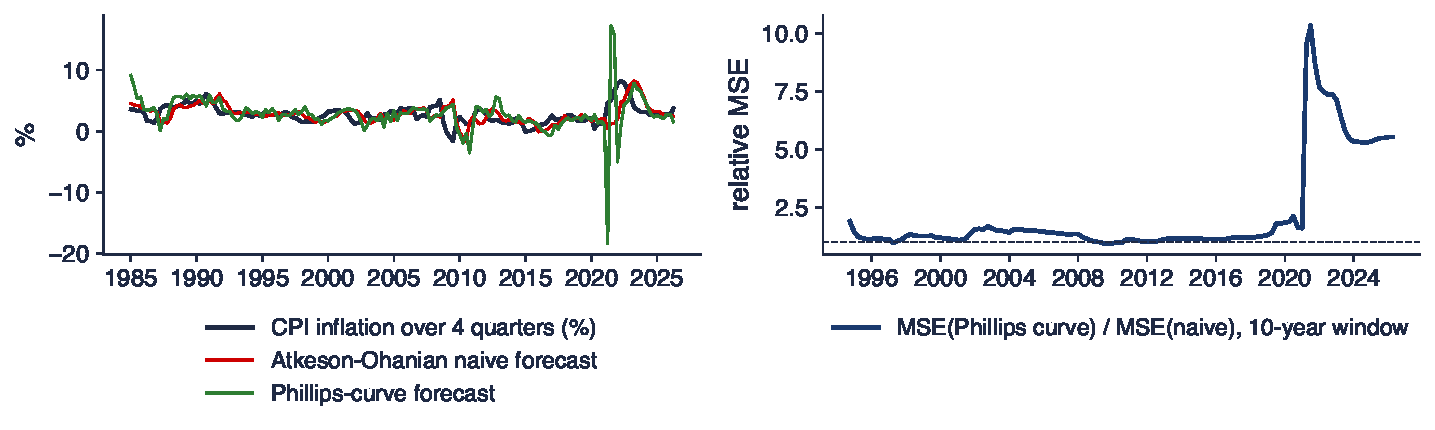
\includegraphics[width=0.97\textwidth,height=0.55\textheight,keepaspectratio]{ats_ch1_ao.pdf}
\end{center}
\vspace{-0.25cm}
\begin{itemize}
    \item Left: four-quarter CPI inflation and the two forecasts made four quarters earlier; right: MSE ratio on a moving 10-year window
\end{itemize}
\quantlet{ATS\_ch1\_dm\_tests}{\qlurl{ATS_ch1_dm_tests}}
\end{frame}

\begin{frame}{Interpreting the Atkeson--Ohanian update}
\itemsize{\small}
\begin{itemize}
    \item RMSE: naive 1.69, Phillips curve 2.97 (ratio 1.75); by period: 1.29 (1985--2007), 1.10 (2008--2019), 2.38 (2020--2026)
    \item Yet DM--HLN = 1.16, $p$ 0.248: the large post-2020 errors inflate the HAC variance as much as the mean
    \begin{itemize}
        \item the moving ratio peaks at 10.3 in 2021Q3: the Phillips curve extrapolated the pandemic unemployment spike
    \end{itemize}
    \item GW: p-value 0.355 with the lagged differential, 0.322 with unemployment
    \begin{itemize}
        \item encompassing, $H_0$ ``the naive forecast encompasses the Phillips curve'': p-value 0.289
        \item encompassing, $H_0$ ``the Phillips curve encompasses the naive forecast'': p-value 0.118
    \end{itemize}
    \item The AO conclusion holds in point estimates, and a test on 41 years of overlapping data cannot separate the two
\end{itemize}
\end{frame}

\begin{frame}{Many models: data snooping, the reality check and SPA}
\itemsize{\small}
\begin{itemize}
    \item Testing $k$ models against a benchmark and reporting the best $p$-value is \textbf{data snooping}
    \begin{itemize}
        \item $H_0$: $\max_{j \le k}\E[d_{j,t}] \le 0$ with $d_{j,t} = L_{0,t} - L_{j,t}$: no model beats the benchmark
        \item $L_{0,t}$: the loss of the benchmark; $L_{j,t}$: the loss of model $j$; $d_{j,t} > 0$: model $j$ did better at $t$
    \end{itemize}
    \item \textbf{Reality check} \refWhite: statistic $\max_j\sqrt P\bar d_j$, $p$-value from the stationary bootstrap (\atschlink{https://danpele.github.io/Advanced-Time-Series/EN/Courses/chapter0_refresher_inference.pdf}{Chapter 0}) under the least favourable configuration
    \begin{itemize}
        \item conservative: very poor models inflate the null distribution
    \end{itemize}
    \item \textbf{SPA} \refHan: studentise each $\bar d_j$ and drop clearly inferior models from the null distribution (consistent $p$-value)
    \begin{itemize}
        \item lower and upper $p$-values bracket it; the upper one equals the RC with studentisation
        \item StepM \refRWze\ identifies \emph{which} models beat the benchmark
    \end{itemize}
    \item EUR/RON, $k = 9$ models (the seven of the table, AR(2) and AR(3)) against the random walk: SPA $p$ = 0.53 (lower), 0.85 (consistent), 0.88 (upper): no model beats it
\end{itemize}
\end{frame}

\begin{frame}{The model confidence set (1/2)}
\itemsize{\small}
\begin{itemize}
    \item \textbf{MCS} \refHLNaa: the set $\hat{\mathcal M}_{1-\alpha}$ that contains the best model(s) with probability at least $1 - \alpha$ asymptotically
    \begin{itemize}
        \item no benchmark: all models are treated symmetrically; analogous to a confidence interval for a parameter
    \end{itemize}
    \item Equivalence test on the $m$ models still in the set
    \begin{itemize}
        \item $H_0$: $\E[d_{i\cdot,t}] = 0$ for all $i$, $\quad d_{i\cdot,t} = L_{i,t} - \frac1m\sum_j L_{j,t}$
        \item $d_{i\cdot,t}$: the loss of model $i$ minus the average loss of all models; positive: model $i$ is worse than average
        \item statistic $T_{\max} = \max_i t_i$, $t_i = \bar d_{i\cdot}/\widehat{\mathrm{se}}(\bar d_{i\cdot})$: the worst model relative to the average, standardised
    \end{itemize}
\end{itemize}
\end{frame}

\begin{frame}{The model confidence set (2/2)}
\itemsize{\small}
\begin{itemize}
    \item Algorithm: start with all models
    \begin{itemize}
        \item if the equivalence test rejects, \textbf{eliminate} the model with the largest $t_i$ and repeat; stop at the first non-rejection
        \item a block bootstrap gives the null distribution and the standard errors
        \item MCS $p$-value of a model: the largest test $p$-value up to its elimination; it stays in $\hat{\mathcal M}_{1-\alpha}$ if this is above $\alpha$
    \end{itemize}
    \item A large MCS is a finding too
    \begin{itemize}
        \item the data cannot separate the models (a weak sample, not equal models)
    \end{itemize}
\end{itemize}
\end{frame}

\begin{frame}{Case study: day-ahead electricity load in Romania}
\itemsize{\footnotesize}
\begin{columns}[T]
\begin{column}{0.36\textwidth}
\centering
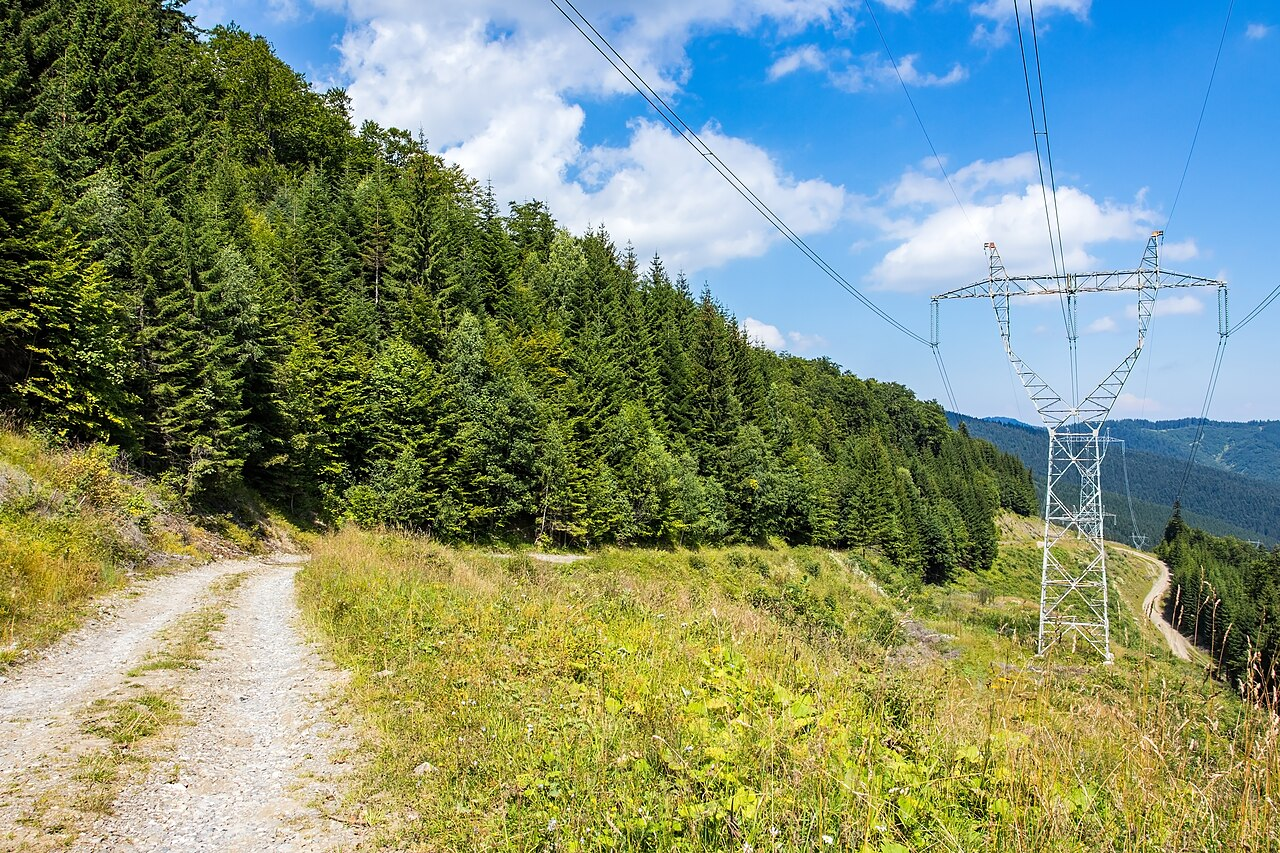
\includegraphics[height=0.36\textheight]{ch1_pylon_predelus_2018.jpg}\\[1mm]
\imgcap{A 400 kV line, Predeluș Pass (2018)}
\imgcredit{https://commons.wikimedia.org/wiki/File:Delta_pylon_Pasul_Predelu\%C8\%99_RO_2018_-_1.jpg}{Photo: Drprv (2018); CC BY-SA 3.0; Wikimedia Commons}
\end{column}
\begin{column}{0.62\textwidth}
\begin{itemize}
    \item Target: the 24 hourly loads of day $d + 1$ with data up to day $d$; 1 January 2025 to 30 September 2026 ($638$ days); mean 5.98 GW
    \begin{itemize}
        \item quantile forecasts at the 99 percentiles, scored by the average pinball loss as in GEFCom2014 \refGEF, \refHF
    \end{itemize}
    \item Models: naive day, weekly naive, mean of 4 weeks; the \textbf{expert ARX} of \refZW\ for each hour
    \begin{itemize}
        \item regressors: $y_{d,h}, y_{d-1,h}, y_{d-6,h}$, min and max of day $d$, last hour of $d$, Monday, Saturday, Sunday; one-year rolling window
        \item quantiles: point forecast plus the empirical quantiles of the last 182 errors at the same hour
    \end{itemize}
    \item ARX: autoregression with exogenous variables (here calendar dummies)
\end{itemize}
\end{column}
\end{columns}
\end{frame}

\begin{frame}{A winter week of load forecasts}
\itemsize{\footnotesize}
\begin{center}
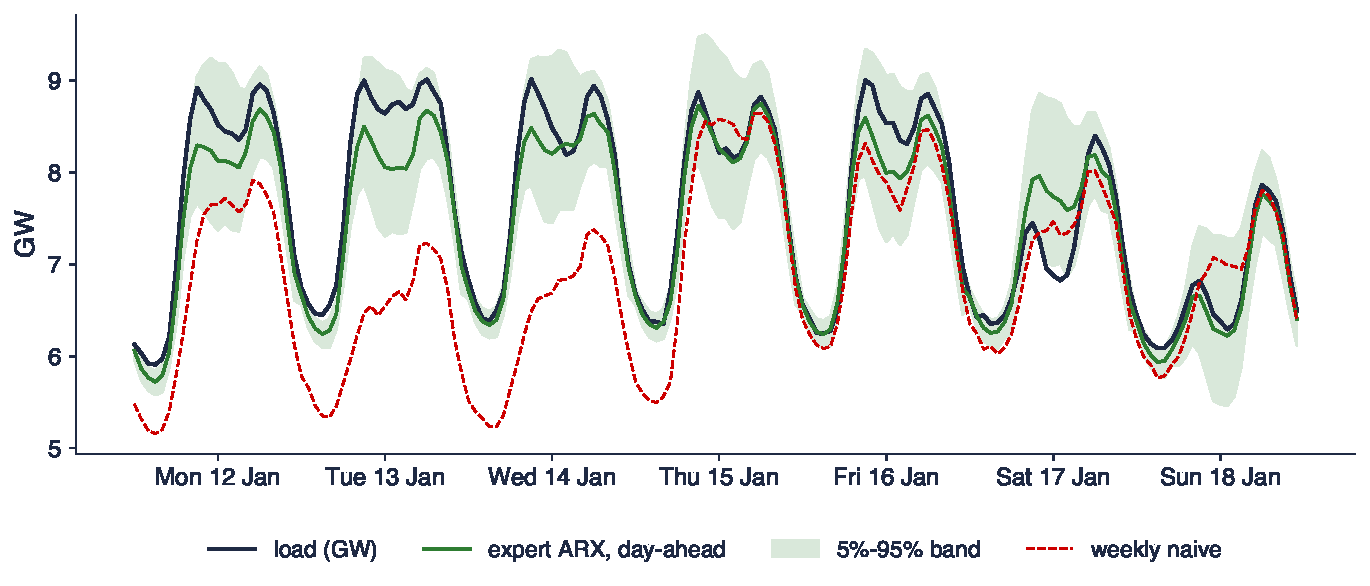
\includegraphics[width=0.97\textwidth,height=0.65\textheight,keepaspectratio]{ats_ch1_load_week.pdf}
\end{center}
\vspace{-0.25cm}
\begin{itemize}
    \item 12--18 January 2026; the weekly naive forecast copies the holiday week of 5--9 January (Orthodox Epiphany and St John, 6--7 January)
\end{itemize}
\quantlet{ATS\_ch1\_load\_mcs}{\qlurl{ATS_ch1_load_mcs}}
\end{frame}

\begin{frame}{Average pinball loss and the 90\% MCS}
\itemsize{\footnotesize}
\begin{center}
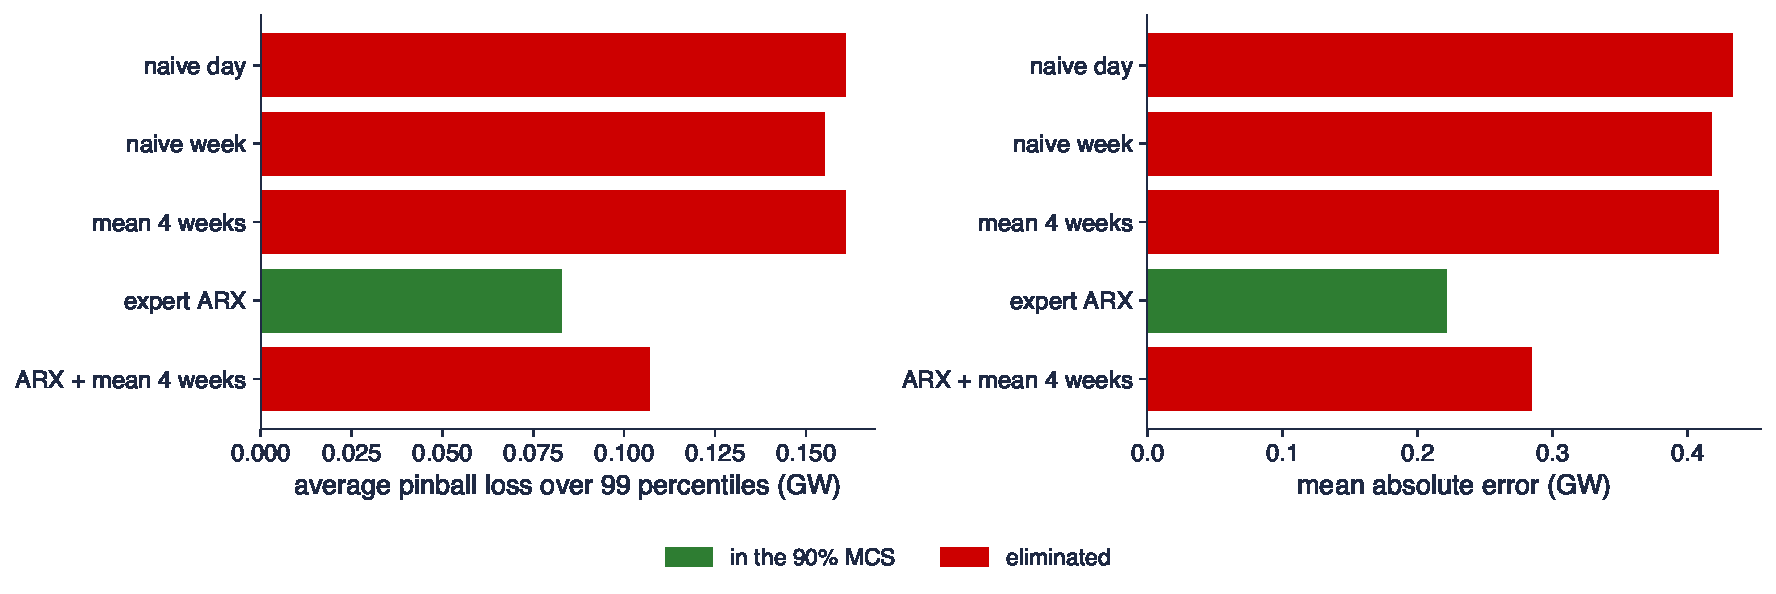
\includegraphics[width=0.97\textwidth,height=0.62\textheight,keepaspectratio]{ats_ch1_load_mcs.pdf}
\end{center}
\vspace{-0.25cm}
\begin{itemize}
    \item Daily average losses; MCS with $T_{\max}$, moving-block bootstrap (blocks of 7 days), 2000 replications; green: in the MCS
\end{itemize}
\quantlet{ATS\_ch1\_load\_mcs}{\qlurl{ATS_ch1_load_mcs}}
\end{frame}

\begin{frame}{Interpreting the load comparison}
\itemsize{\footnotesize}
\begin{center}
\scriptsize
\begin{tabular}{lrrrr}
\toprule
\textbf{Model} & \textbf{Pinball (MW)} & \textbf{MAE (MW)} & \textbf{90\% coverage} & \textbf{MCS $p$} \\
\midrule
naive (day $d$) & 161 & 433 & 89.2\% & $<$\,0.001 \\
weekly naive & 155 & 417 & 87.6\% & $<$\,0.001 \\
mean of 4 weeks & 161 & 423 & 88.7\% & $<$\,0.001 \\
expert ARX & 83 & 221 & 88.2\% & 1.000 \\
ARX + mean of 4 weeks & 107 & 285 & 88.3\% & $<$\,0.001 \\
\bottomrule
\end{tabular}
\end{center}
\begin{itemize}
    \item The expert ARX halves the losses of the naive rules and is alone in the MCS; DM--HLN against the ARX + mean combination: \ensuremath{-}10.7
    \item Here combining with a much worse forecast hurts: equal weights help only when the forecasts are of similar quality (Section 5)
    \item All intervals under-cover slightly; the largest losses fall on and right after public holidays (8 January 2026, 25 December 2025, 1 January 2025): calendar effects are the next improvement
\end{itemize}
\end{frame}

\begin{frame}{Recap: Comparing forecasts}
\itemsize{\small}
\begin{itemize}
    \item DM compares forecasts; with estimated models choose West (population) or GW (methods, rolling window)
    \item Multi-step, small $P$: HAC variance plus the HLN correction and $t_{P-1}$
    \item Nested models: Clark--West; many models: SPA or the MCS, never the best $p$-value
    \item Romanian inflation, US inflation, EUR/RON: the simple benchmark is hard to beat and differences are rarely significant
\end{itemize}
\end{frame}


%=============================================================================
\section{Forecast combination}
%=============================================================================

\begin{frame}{Bates and Granger (1969)}
\itemsize{\footnotesize}
\begin{columns}[T]
\begin{column}{0.30\textwidth}
\centering
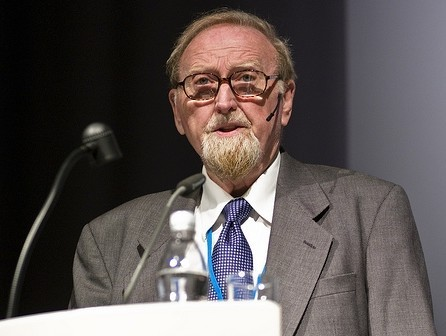
\includegraphics[height=0.32\textheight]{ch1_granger_2008.jpg}\\[1mm]
\imgcap{Clive W.~J.\ Granger (1934--2009), Nobel Memorial Prize 2003}
\imgcredit{https://commons.wikimedia.org/wiki/File:Clive_Granger_by_Olaf_Storbeck.jpg}{Photo: Olaf Storbeck (2008); CC BY-SA 2.0; Wikimedia Commons}
\end{column}
\begin{column}{0.68\textwidth}
\begin{itemize}
    \item Two unbiased forecasts with error variances $\sigma_1^2, \sigma_2^2$ and covariance $\sigma_{12}$; combination $w\hat y_1 + (1 - w)\hat y_2$ \refBG
    \begin{itemize}
        \item error variance $w^2\sigma_1^2 + (1 - w)^2\sigma_2^2 + 2w(1 - w)\sigma_{12}$, minimised at
        \item $w^* = \dfrac{\sigma_2^2 - \sigma_{12}}{\sigma_1^2 + \sigma_2^2 - 2\sigma_{12}}$, \quad $\sigma^2_c = \dfrac{\sigma_1^2\sigma_2^2 - \sigma_{12}^2}{\sigma_1^2 + \sigma_2^2 - 2\sigma_{12}} \le \min(\sigma_1^2, \sigma_2^2)$
        \item $\sigma^2_c$: the error variance of the optimal combination, never above that of the better forecast; the less precise forecast gets the smaller weight
    \end{itemize}
    \item $N$ forecasts: $\mathbf w^* = \Sigma^{-1}\iota/(\iota'\Sigma^{-1}\iota)$, with $\Sigma$ the covariance matrix of the errors and $\iota$ a vector of ones; \refGRm: regress $y$ on the forecasts, with or without a constant and the sum-to-one restriction
    \begin{itemize}
        \item combination diversifies model risk, structural breaks and the private information of forecasters \refTim
    \end{itemize}
\end{itemize}
\end{column}
\end{columns}
\end{frame}

\begin{frame}{The forecast combination puzzle}
\itemsize{\small}
\begin{itemize}
    \item Empirical regularity: the simple average beats the ``optimal'' estimated weights \refSWzd, \refTim, \refGKMT
    \begin{itemize}
        \item Stock--Watson: across 7 countries and many predictors of output growth, equal weights and the median are among the best combinations
    \end{itemize}
    \item \textbf{Explanation} \refSWal, \refCMVW: the weights are estimated
    \begin{itemize}
        \item $\E[\mathrm{MSE}(\hat w)] = \mathrm{MSE}(w^*) + \E(\hat w - w^*)^2 D$, $D = \sigma_1^2 + \sigma_2^2 - 2\sigma_{12}$ (the variance of $e_1 - e_2$)
        \item $\hat w$: the weight estimated from $n$ past errors; MSE: the mean squared error of the combination
        \item gain of $w^*$ over $1/2$: $(w^* - 1/2)^2D$; loss from estimating: $\mathrm{Var}(\hat w)D$, of order $1/n$
        \item equal weights win when $(w^* - 1/2)^2 < \mathrm{Var}(\hat w)$: similar forecasts, short samples, correlated errors
    \end{itemize}
    \item Also: weights move with breaks, so long windows are biased and short ones noisy
\end{itemize}
\end{frame}

\begin{frame}{The puzzle by simulation}
\itemsize{\footnotesize}
\begin{center}
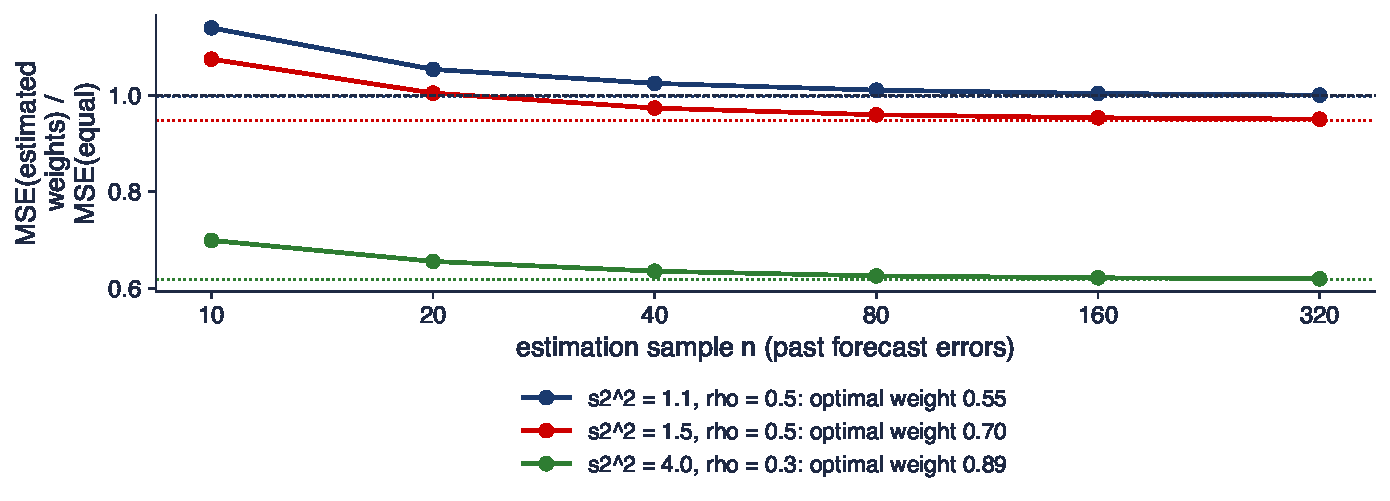
\includegraphics[width=0.97\textwidth,height=0.64\textheight,keepaspectratio]{ats_ch1_puzzle.pdf}
\end{center}
\vspace{-0.25cm}
\begin{itemize}
    \item Bivariate Normal errors with $\sigma_1^2 = 1$; weights estimated from $n$ past errors; 4\,000 replications; dotted: population ratio $\mathrm{MSE}(w^*)/\mathrm{MSE}(1/2)$
\end{itemize}
\quantlet{ATS\_ch1\_combination}{\qlurl{ATS_ch1_combination}}
\end{frame}

\begin{frame}{Interpreting the puzzle simulation}
\itemsize{\small}
\begin{itemize}
    \item Similar forecasts ($w^* = 0.55$): the optimal weight lowers the population MSE only to 0.997 of the equal-weight MSE, while estimating it costs: ratio 1.14 at $n = 10$, 1.024 at $n = 40$
    \item Moderately different ($w^* = 0.70$): estimated weights need about 20 past errors to break even (1.07 at $n = 10$, 0.973 at $n = 40$)
    \item Very different ($w^* = 0.89$): estimate the weights, or drop the weak forecast; the load case of Section 4 is of this kind
\end{itemize}
\end{frame}

\begin{frame}{Between equal and optimal: shrinkage and robust combinations}
\itemsize{\small}
\begin{itemize}
    \item \textbf{Shrinkage}: $\hat w_\lambda = \lambda\hat w + (1 - \lambda)\iota/N$ \refDP, \refSWzd
    \begin{itemize}
        \item $\hat w$: the estimated weights; $\iota/N$: equal weights for $N$ forecasts; $\lambda \in [0,1]$: $\lambda = 0$ gives the mean, $\lambda = 1$ the estimated weights
        \item a Bayesian prior centred on equal weights; $\lambda$ falls with the number of forecasts and rises with the sample
    \end{itemize}
    \item \textbf{Performance weights}: $w_i \propto 1/\mathrm{MSE}_i$ on a recent window, ignoring correlations; discounting gives recent errors more weight
    \begin{itemize}
        \item \textbf{previous best}: select the forecaster with the lowest past MSE (a weight of one)
    \end{itemize}
    \item \textbf{Robust}: median, trimmed mean: protect against outlying forecasters
    \item Panels of experts change: forecasters enter and exit, so $\Sigma$ is never fully observed \refCT
    \begin{itemize}
        \item performance weights need a minimum record; a review of 50 years of practice: \refWHLK
    \end{itemize}
\end{itemize}
\end{frame}

\begin{frame}{Combining density forecasts}
\itemsize{\small}
\begin{itemize}
    \item \textbf{Linear pool}: $p(y) = \sum_i w_ip_i(y)$, $w_i \ge 0$, $\sum w_i = 1$ \refHM
    \begin{itemize}
        \item $p_i$: the density forecast of model $i$; $w_i$: its weight; the pool is a mixture of the densities
        \item weights that minimise the average log score: \textbf{optimal prediction pools} \refGA
        \item interior weights even when every model is misspecified: a pool is not a model average in the Bayesian sense
    \end{itemize}
    \item The linear pool of calibrated densities is \textbf{over-dispersed} \refGRjac
    \begin{itemize}
        \item the mixture adds the variance of the means; remedy: a beta-transformed pool or quantile averaging (Vincentisation)
    \end{itemize}
    \item Proper scores (Section 3) are the natural criteria for estimating and comparing pools
\end{itemize}
\end{frame}

\begin{frame}{Optimal pools for the S\&P 500 densities}
\itemsize{\footnotesize}
\begin{center}
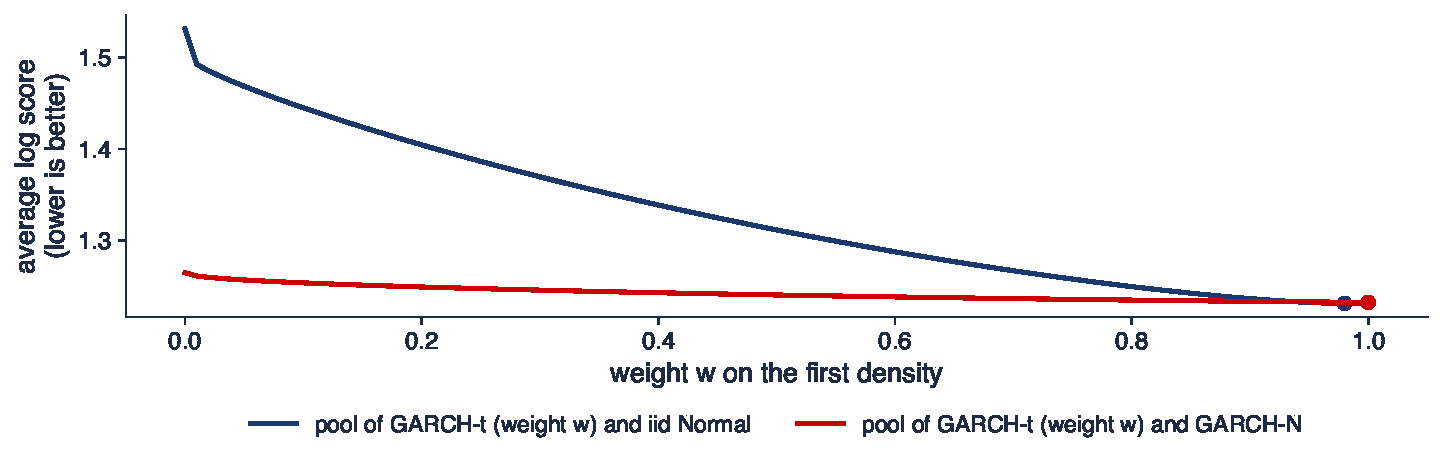
\includegraphics[width=0.97\textwidth,height=0.59\textheight,keepaspectratio]{ats_ch1_pool.pdf}
\end{center}
\vspace{-0.25cm}
\begin{itemize}
    \item Average log score of $wp_{\mathrm{GARCH}\text{-}t} + (1 - w)p_2$ on 2013--2026; dots: minima
    \item With the i.i.d.\ Normal: $w^* = 0.98$, score 1.2318 against 1.2328 for GARCH-$t$ alone; with GARCH-N: $w^* = 1.00$: GARCH-$t$ dominates, the pool adds almost nothing
\end{itemize}
\quantlet{ATS\_ch1\_density\_forecasts}{\qlurl{ATS_ch1_density_forecasts}}
\end{frame}

\begin{frame}{Interpreting the optimal pools}
\itemsize{\small}
\begin{itemize}
    \item The pool with the i.i.d.\ Normal puts almost all weight on GARCH-$t$: a small Normal component only insures against extreme days
    \item With GARCH-N the optimum is the corner $w = 1$: the two GARCH densities carry the same information, the $t$ tails are simply better
    \item Weights estimated on the evaluation sample are optimistic; in practice estimate them on a past window and evaluate on the next
\end{itemize}
\end{frame}

\begin{frame}{Case study: combination schemes against the simple average}
\itemsize{\footnotesize}
\begin{columns}[T]
\begin{column}{0.32\textwidth}
\centering
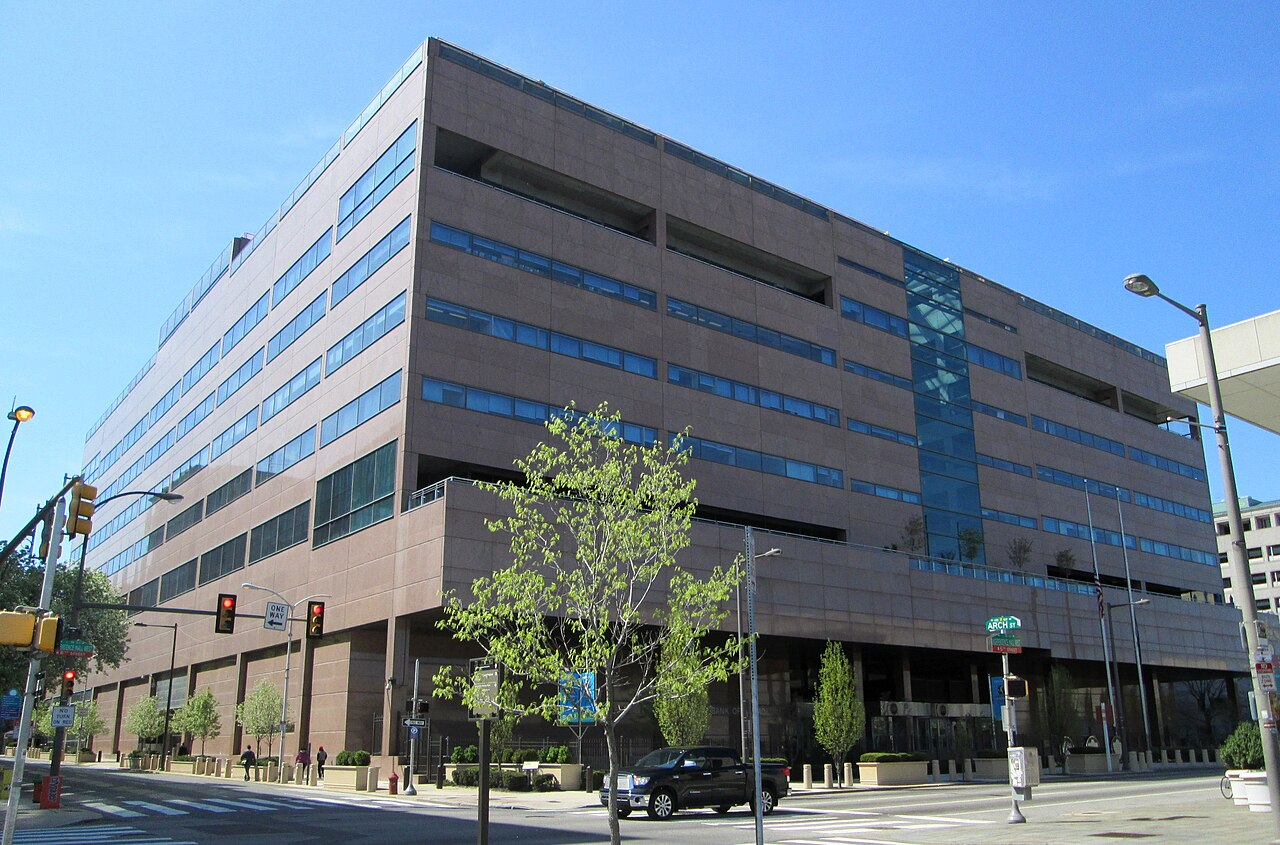
\includegraphics[height=0.30\textheight]{ch1_fed_philadelphia_2013.jpg}\\[1mm]
\imgcap{Federal Reserve Bank of Philadelphia, home of the SPF since 1990}
\imgcredit{https://commons.wikimedia.org/wiki/File:Federal_Reserve_Bank_Building_Philadelphia.jpg}{Photo: Beyond My Ken (2013); CC BY-SA 4.0; Wikimedia Commons}
\end{column}
\begin{column}{0.66\textwidth}
\begin{itemize}
    \item \refGKMT\ compare combination schemes on the ECB Survey of Professional Forecasters: equal weights, median, trimmed mean, performance-based weights, shrinkage, and others
    \begin{itemize}
        \item their answer: rarely, and not robustly over time
    \end{itemize}
    \item We apply their schemes to the US SPF: CPI inflation (annualised q/q) four quarters after the survey quarter; surveys 1990Q1--2025Q2 ($P = 142$, 195 forecasters, on average 36 per survey)
    \begin{itemize}
        \item performance weights: inverse MSE over the last 20 surveys with a known outcome, at least 8 past forecasts (on average 25 eligible); trimmed mean: 10\% on each side
    \end{itemize}
\end{itemize}
\end{column}
\end{columns}
\end{frame}

\begin{frame}{Individual SPF forecasts and the outcome}
\itemsize{\footnotesize}
\begin{center}
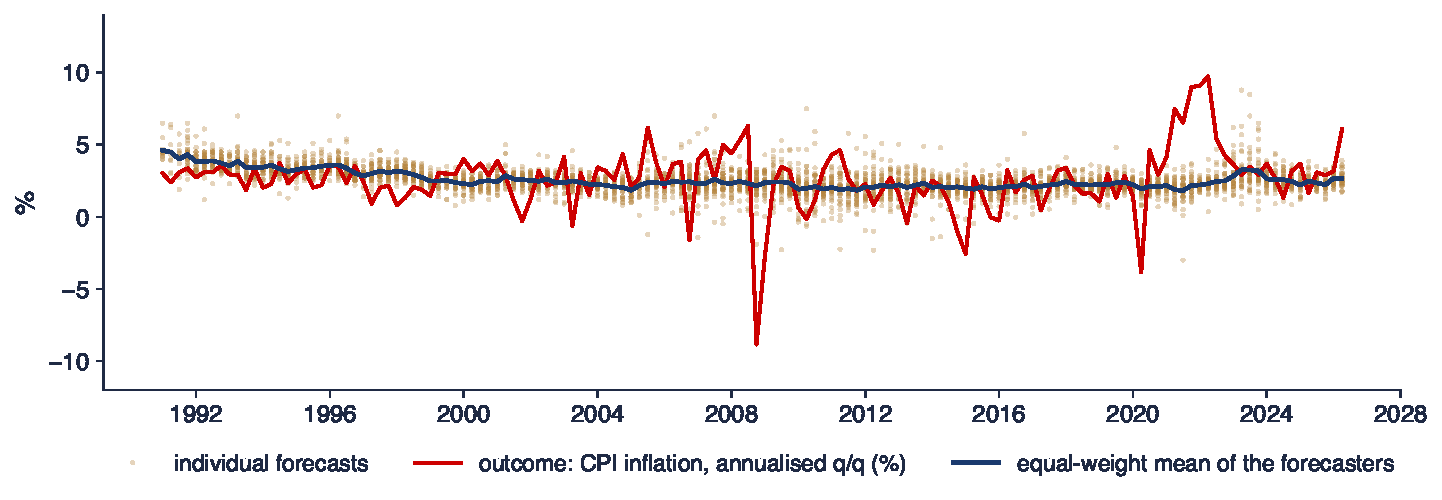
\includegraphics[width=0.97\textwidth,height=0.64\textheight,keepaspectratio]{ats_ch1_spf.pdf}
\end{center}
\vspace{-0.25cm}
\begin{itemize}
    \item Each dot: one forecaster's CPI forecast for the quarter four quarters ahead, placed at the target quarter; the outcome is far more volatile than any forecast
\end{itemize}
\quantlet{ATS\_ch1\_spf\_combination}{\qlurl{ATS_ch1_spf_combination}}
\end{frame}

\begin{frame}{Combination schemes against the mean}
\itemsize{\footnotesize}
\begin{center}
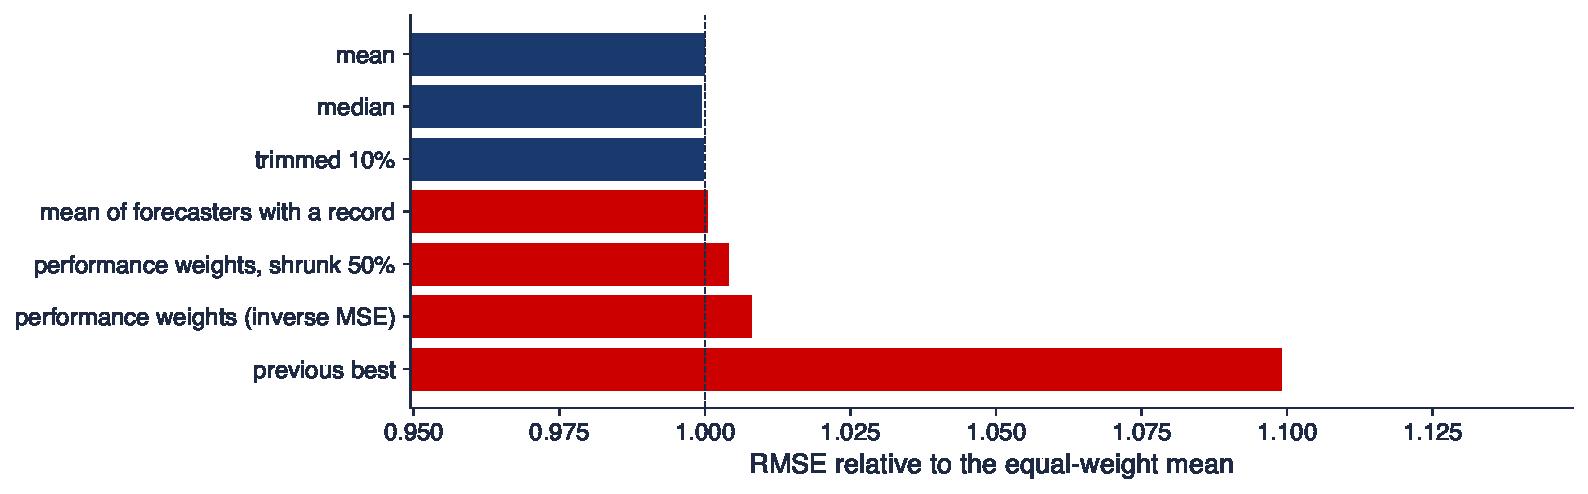
\includegraphics[width=0.97\textwidth,height=0.56\textheight,keepaspectratio]{ats_ch1_spf_schemes.pdf}
\end{center}
\vspace{-0.25cm}
\begin{itemize}
    \item RMSE relative to the equal-weight mean (RMSE 2.18 pp); blue: at least as good as the mean
\end{itemize}
\quantlet{ATS\_ch1\_spf\_combination}{\qlurl{ATS_ch1_spf_combination}}
\end{frame}

\begin{frame}{Interpreting the SPF combination}
\itemsize{\footnotesize}
\begin{itemize}
    \item Median 0.999, trimmed mean 1.000, inverse-MSE 1.008, previous best 1.099 (relative RMSE)
    \begin{itemize}
        \item DM--HLN against the mean: median $p$ 0.842; inverse MSE $p$ 0.091; previous best HLN 2.76, $p$ 0.007
        \item The answer of \refGKMT\ holds on US data: nothing beats the average significantly, and chasing the past winner loses
    \end{itemize}
    \item Yet 33\% of the 76 forecasters with at least 20 forecasts have a lower RMSE than the mean
    \begin{itemize}
        \item they are known only ex post, over different and shorter samples: survivorship and luck, not skill one could have selected
    \end{itemize}
    \item Mincer--Zarnowitz on the mean: $\hat b = 0.24$ (SE 0.31), $R^2 = 0.005$, $p$ $<$\,0.001: one-year-ahead quarterly CPI inflation is almost unpredictable; the forecasts are smooth, the outcomes noisy
\end{itemize}
\end{frame}

\begin{frame}{Lessons from the M4 and M5 competitions}
\itemsize{\small}
\begin{itemize}
    \item \textbf{M4} (2018) \refMd: 100\,000 series, 61 methods, point forecasts and 95\% intervals
    \begin{itemize}
        \item the winner was a hybrid of exponential smoothing and a recurrent neural network; the second, a combination of statistical methods with weights learned by a meta-learner
        \item combinations dominated the top places; pure machine learning methods did poorly; prediction intervals were too narrow for most methods
    \end{itemize}
    \item \textbf{M5} (2020) \refMe: 42\,840 hierarchical Walmart sales series, weighted scaled errors
    \begin{itemize}
        \item gradient-boosted trees (LightGBM) trained \emph{across} series won; exogenous variables (prices, events) and cross-learning mattered
        \item again, ensembles of many models were at the top (\atschlink{https://danpele.github.io/Advanced-Time-Series/EN/Courses/chapter12_machine_learning_deep_learning.pdf}{Chapter 12})
    \end{itemize}
    \item Common lesson: combine, evaluate with scale-free scores (MASE, \atschlink{https://danpele.github.io/Time-Series-Analysis/EN/Courses/chapter0_introduction.pdf}{Chapter 0 of TSA}) and proper scores, and report uncertainty that is calibrated
\end{itemize}
\end{frame}

\begin{frame}{Recap: Combination}
\itemsize{\small}
\begin{itemize}
    \item Optimal weights reduce the error variance; estimated weights add a cost of order $1/n$
    \item The puzzle: when forecasts are similar, equal weights, the median and the trimmed mean win
    \item Linear pools of densities are over-dispersed; estimate them by the log score
    \item US SPF: no scheme beats the mean significantly; selecting the past winner loses
\end{itemize}
\end{frame}


%=============================================================================
\section{Real-time data}
%=============================================================================

\begin{frame}{Vintages and revisions}
\itemsize{\small}
\begin{itemize}
    \item Macroeconomic data are revised: US GDP is first published about 30 days after the quarter and revised for years (benchmark revisions, new methods)
    \begin{itemize}
        \item a \textbf{vintage} is the data set as available on a given date; the real-time data set stores all vintages \refCS
    \end{itemize}
    \item Sources without a key: ALFRED (St.\ Louis Fed, vintages of FRED series), the Philadelphia Fed RTDSM; the ECB keeps a real-time database for the euro area; INS publishes a flash estimate of GDP and later revised estimates
    \begin{itemize}
        \item forecasts made with latest-vintage data overstate what was predictable in real time \refSC, \refCr
    \end{itemize}
    \item Question for the evaluation: which vintage is the ``truth''? The first release (what forecasters target) or the latest (the best estimate of reality)?
\end{itemize}
\end{frame}

\begin{frame}{US real GDP growth: first release and latest vintage}
\itemsize{\footnotesize}
\begin{center}
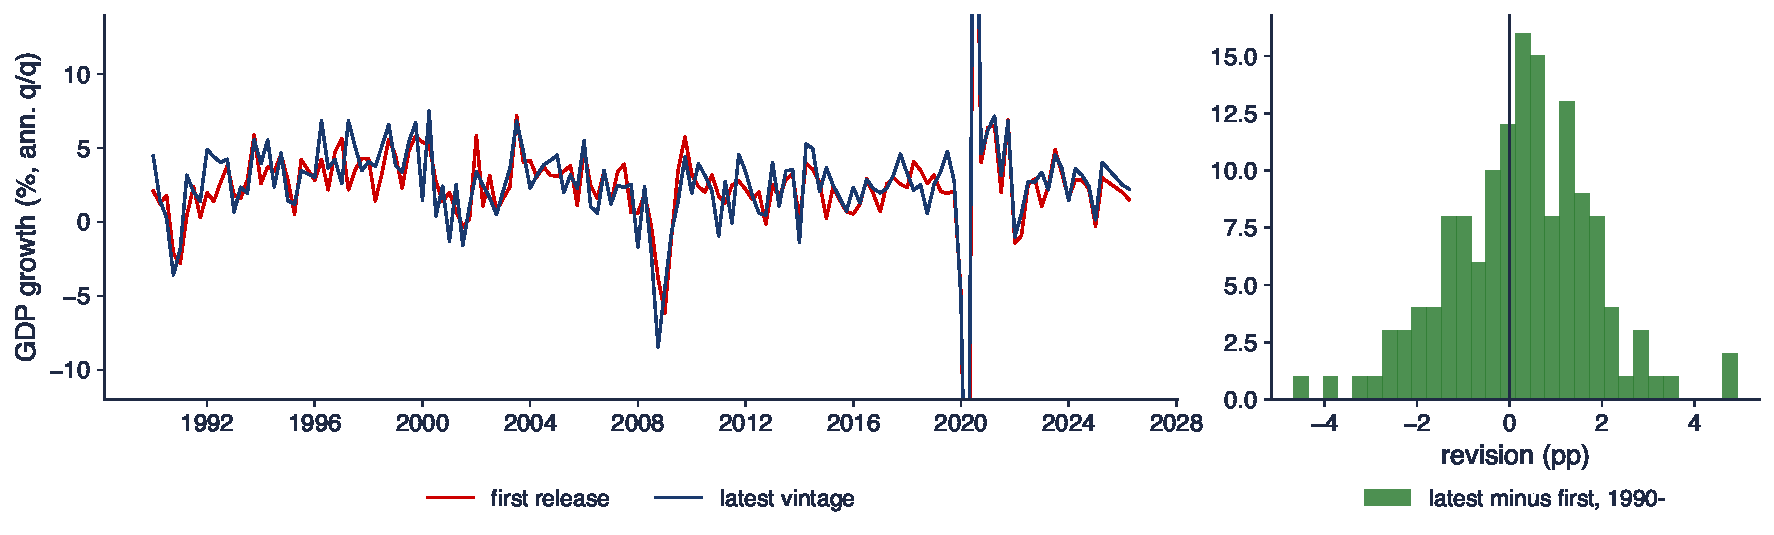
\includegraphics[width=0.97\textwidth,height=0.56\textheight,keepaspectratio]{ats_ch1_realtime.pdf}
\end{center}
\vspace{-0.25cm}
\begin{itemize}
    \item Annualised q/q growth, 1990--2026; revisions = latest minus first release (Philadelphia Fed RTDSM); the 2025Q4 first release is missing (government shutdown)
\end{itemize}
\quantlet{ATS\_ch1\_real\_time}{\qlurl{ATS_ch1_real_time}}
\end{frame}

\begin{frame}{Interpreting the revisions}
\itemsize{\small}
\begin{itemize}
    \item Mean revision 0.23 pp, standard deviation 1.54 pp, mean absolute revision 1.21 pp over 143 quarters; correlation first--latest 0.939
    \begin{itemize}
        \item largest: 2020Q2 (4.9 pp) and 2008Q4 (\ensuremath{-}4.7 pp): revisions are large exactly at turning points
    \end{itemize}
    \item SPF current-quarter nowcast ($P = 143$): RMSE 1.95 against the first release, 2.36 against the latest; MZ slope 1.15 and 1.08
    \item The ranking of forecasters and models can change with the vintage: state the choice in the pre-registration
\end{itemize}
\end{frame}

\begin{frame}{A pre-registered evaluation design}
\itemsize{\small}
\begin{itemize}
    \item Fix \textbf{before} looking at the out-of-sample results
    \begin{itemize}
        \item target, horizons, loss or score (Sections 1--3), vintage of the outcome, evaluation period, estimation scheme and window
        \item benchmark (random walk, seasonal naive, survey mean) and the full list of competing models
        \item tests: DM--HLN or GW; Clark--West if nested; SPA or MCS for many models; a correction for several horizons (Holm)
    \end{itemize}
    \item Report everything that was tried; a model selected on the test period has a biased error
    \begin{itemize}
        \item the project of this course starts with exactly such a plan (proposal and pre-registration, 5\%)
    \end{itemize}
\end{itemize}
\end{frame}

\begin{frame}{Recap: Real-time data}
\itemsize{\small}
\begin{itemize}
    \item Evaluate forecasts with the data that existed when they were made
    \item Revisions are large at turning points; the choice of the ``truth'' vintage changes RMSE and rankings
    \item Pre-register targets, losses, benchmarks, tests and the vintage
\end{itemize}
\end{frame}


%=============================================================================
\section{AI for scientific discovery}
%=============================================================================

\begin{frame}{An open question}
\itemsize{\small}
\begin{itemize}
    \item Does the forecast combination puzzle survive when the panel of experts changes over time and the outcome distribution shifts (2020--2023)?
    \begin{itemize}
        \item formal: $H_0$: $\E[(y - \hat y_{\lambda})^2 - (y - \bar y)^2] \ge 0$ for every shrinkage factor $\lambda$ fixed in advance, in every sub-period
        \item $\hat y_\lambda$: the shrinkage combination with factor $\lambda$; $\bar y$: the mean of all forecasters
        \item falsified by a pre-registered $\lambda$ that beats the mean with DM--HLN $p < 0.05$ after a Holm correction across sub-periods
    \end{itemize}
    \item Why it matters: central banks publish the survey mean; a better combination would change the published expectations
    \begin{itemize}
        \item literature to start from: \refGKMT, \refCT, \refSWal, \refCMVW, \refWHLK
    \end{itemize}
\end{itemize}
\end{frame}

\begin{frame}{The discovery loop with an AI assistant}
\itemsize{\footnotesize}
\begin{itemize}
    \item An AI assistant (an LLM such as Claude, ChatGPT, Gemini or Copilot) speeds up each step; Semantic Scholar and Elicit help with the literature
    \begin{itemize}
        \item \textbf{literature}: \aiprompt{List peer-reviewed papers on combining SPF forecasts with entry and exit of forecasters; give DOIs.} Then check every DOI on Crossref
        \item \textbf{hypothesis}: \aiprompt{Propose three reasons why inverse-MSE weights could beat the mean after 2020, each with a test.}
        \item \textbf{code and replication}: ask for a function, then reproduce a known number first (the relative RMSE of the median in this lecture)
        \item \textbf{robustness and critique}: \aiprompt{Act as a hostile referee: list every way this evaluation could be data-snooped.}
    \end{itemize}
    \item Report: what was asked, what was kept, what was rejected (AI\_USE.md, AI\_ERRORS.md)
\end{itemize}
\end{frame}

\begin{frame}{Required checks}
\itemsize{\small}
\begin{itemize}
    \item Every reference exists and says what is claimed (DOI resolves, title matches, the result is in the paper)
    \item No look-ahead: weights at survey $s$ use only outcomes known at $s$ (here, forecasts from at least five surveys earlier, whose target quarter has ended)
    \item The HAC lag matches the overlap of the targets ($h - 1$); the HLN correction is applied
    \item $\lambda$, sub-periods and the minimum record are fixed before the results; all variants are reported
    \item The interpretation separates ``not significant'' from ``equal''
\end{itemize}
\end{frame}

\begin{frame}{Mini-case: shrinkage across sub-periods}
\itemsize{\footnotesize}
\begin{center}
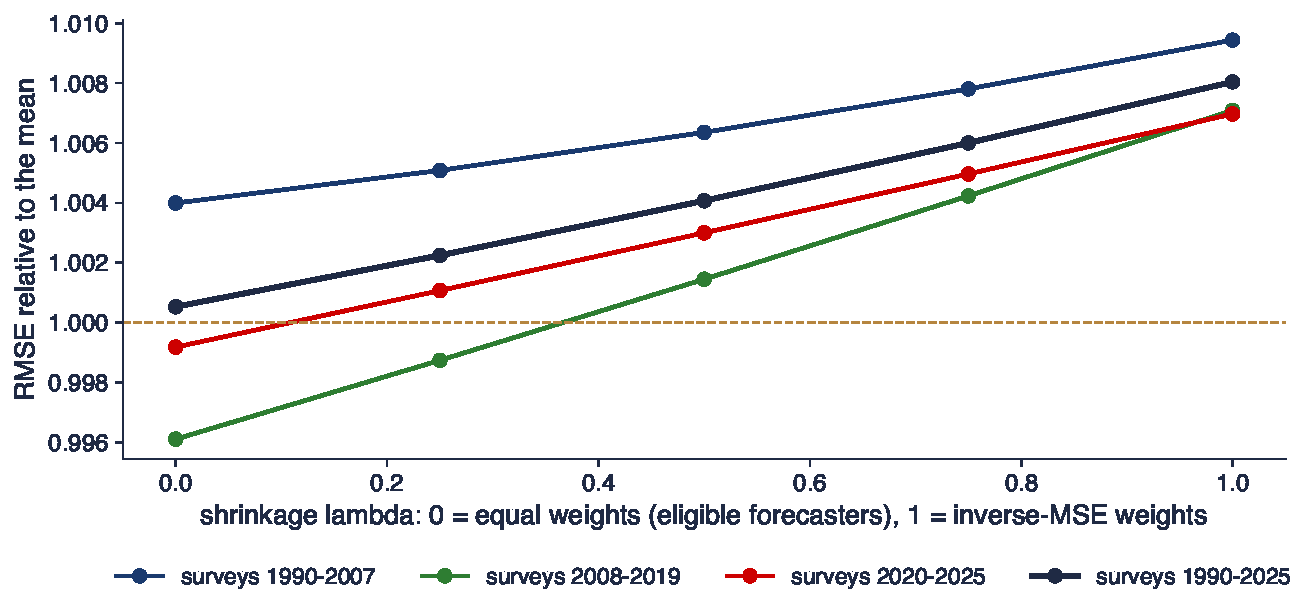
\includegraphics[width=0.97\textwidth,height=0.49\textheight,keepaspectratio]{ats_ch1_ai_case.pdf}
\end{center}
\vspace{-0.25cm}
\begin{itemize}
    \item RMSE of $\lambda\cdot$(inverse-MSE weights) + $(1 - \lambda)\cdot$(equal weights among eligible forecasters), relative to the mean of all forecasters; US SPF, CPI four quarters ahead
    \item $\lambda = 1$: 1.009 (1990--2007, $P = 72$), 1.007 (2008--2019), 1.007 (2020--2025); full sample HLN 1.70, $p$ 0.091
    \item Every sub-period: the more weight on past performance, the worse; the puzzle survives the 2020--2023 inflation surge
\end{itemize}
\quantlet{ATS\_ch1\_spf\_combination}{\qlurl{ATS_ch1_spf_combination}}
\end{frame}

\begin{frame}{Project idea}
\itemsize{\small}
\begin{itemize}
    \item \textbf{Combining Romanian inflation forecasts}: models (AR, Phillips curve with the output gap, BNR target), surveys and market-based expectations
    \begin{itemize}
        \item pre-register horizons 1--12 months, the pinball loss at 5\%, 50\%, 95\% and the CRPS, the Holm correction across horizons
        \item replicate first: the Romanian inflation table of this lecture (Seminar 1, C1 does it by horizon)
        \item extension: density combination by optimal pools; GW test of whether the 2022 shock changed the winner
    \end{itemize}
    \item Deliverables follow the course rules: repository, report, AI\_USE.md, AI\_ERRORS.md, oral defence
\end{itemize}
\end{frame}


%=============================================================================
\section{Wrap-up}
%=============================================================================

\begin{frame}{Key takeaways}
\itemsize{\small}
\begin{itemize}
    \item Choose the loss or score first: it defines what a ``good'' forecast is (mean, median, quantile, distribution)
    \item Density forecasts: check calibration with PIT, rank with proper scores; ES needs VaR to be scored
    \item Tests: DM--HLN with HAC, GW for methods, Clark--West for nested models, SPA and MCS for many
    \item Combine similar forecasts with equal weights; estimated weights pay off only with very different forecasts and long records
    \item Evaluate in real time and pre-register the design
\end{itemize}
\end{frame}

\begin{frame}{Self-assessment}
\itemsize{\small}
\begin{columns}[T]
\begin{column}{0.56\textwidth}
\begin{block}{Questions}
\begin{itemize}
    \item Which functional does the pinball loss with $\tau = 0.05$ elicit?
    \item What does a U-shaped PIT histogram say about the intervals?
    \item Why is DM not valid for nested models with estimated parameters?
    \item When do estimated combination weights beat equal weights?
    \item Why can ES not be ranked on its own?
\end{itemize}
\end{block}
\end{column}
\begin{column}{0.40\textwidth}
\begin{block}{Next: \atschlink{https://danpele.github.io/Advanced-Time-Series/EN/Courses/chapter2_structural_breaks_nonlinear_models.pdf}{Chapter 2}}
\begin{itemize}
    \item Structural breaks and nonlinear models: tests for breaks, threshold models
    \item Forecast evaluation under instability: rolling windows, forecast breakdowns, the fluctuation test \refGRaz
\end{itemize}
\end{block}
\end{column}
\end{columns}
\end{frame}


%=============================================================================
\section{Appendix}
%=============================================================================

\begin{frame}{Appendix: consistency of the pinball loss}
\hypertarget{atsapp1}{}\atsappback{atssrc1}{Back}
\itemsize{\small}
\begin{itemize}
    \item $\E\rho_\tau(Y - x) = \tau\int_x^\infty(y - x)dF(y) + (1 - \tau)\int_{-\infty}^x(x - y)dF(y)$
    \item Derivative (Leibniz): $-\tau(1 - F(x)) + (1 - \tau)F(x) = F(x) - \tau$; zero at $x = F^{-1}(\tau)$; second derivative $f(x) \ge 0$
    \item For $\tau = 1/2$: $\rho_{1/2}(e) = |e|/2$, so the median; for $x$ off the quantile the excess loss is $\int_q^x(F(z) - \tau)dz > 0$
    \item Generalised piecewise linear losses $(\mathbf 1\{y \le x\} - \tau)(g(x) - g(y))$, $g$ increasing, are the whole class of consistent losses for the quantile \refGnaa
\end{itemize}
\end{frame}

\begin{frame}{Appendix: the kernel form of the CRPS}
\hypertarget{atsapp2}{}\atsappback{atssrc2}{Back}
\itemsize{\small}
\begin{itemize}
    \item Write $(F(z) - \mathbf 1\{y \le z\})^2 = F(z)^2 - 2F(z)\mathbf 1\{y \le z\} + \mathbf 1\{y \le z\}$
    \item With $X, X' \sim F$ i.i.d.: $F(z)^2 = P(X \le z, X' \le z)$ and $\E|X - y| = \int[F(z)(1 - \mathbf 1\{y \le z\}) + (1 - F(z))\mathbf 1\{y \le z\}]dz$
    \item $\frac12\E|X - X'| = \int F(z)(1 - F(z))dz$; subtracting gives $\int(F(z) - \mathbf 1\{y \le z\})^2dz$
    \item Propriety: $\E_G\mathrm{CRPS}(F, Y) - \E_G\mathrm{CRPS}(G, Y) = \int(F(z) - G(z))^2dz \ge 0$, zero only if $F = G$
\end{itemize}
\end{frame}

\begin{frame}{Appendix: the Clark--West adjustment}
\hypertarget{atsapp3}{}\atsappback{atssrc3}{Back}
\itemsize{\small}
\begin{itemize}
    \item Under $H_0$ the larger model's extra coefficients $\beta_2 = 0$; its forecast is $\hat y_2 = \hat y_1 + \hat\beta_2'x_{2}$ approximately, with $\hat\beta_2$ pure estimation noise
    \item $e_2 = e_1 - (\hat y_2 - \hat y_1)$, so $e_1^2 - e_2^2 = 2e_1(\hat y_2 - \hat y_1) - (\hat y_2 - \hat y_1)^2$
    \item $\E[e_1(\hat y_2 - \hat y_1)] = 0$ under $H_0$ ($e_1$ is a martingale difference), hence $\E(e_1^2 - e_2^2) = -\E(\hat y_2 - \hat y_1)^2 < 0$
    \item Adding $(\hat y_1 - \hat y_2)^2$ recentres the differential at zero: $f_t = 2e_{1t}(\hat y_{2t} - \hat y_{1t})$, the encompassing statistic of \refHLNih\ in disguise
\end{itemize}
\end{frame}


%=============================================================================
\section{References}
%=============================================================================

\begin{frame}{References (1/7)}
\itemsize{\tiny}
\begin{itemize}
    \item Amisano, G., \& Giacomini, R. (2007). Comparing density forecasts via weighted likelihood ratio tests. \textit{Journal of Business \& Economic Statistics}, 25(2), 177--190. \href{https://doi.org/10.1198/073500106000000332}{doi:10.1198/073500106000000332}
    \item Atkeson, A., \& Ohanian, L. E. (2001). Are Phillips curves useful for forecasting inflation? \textit{Federal Reserve Bank of Minneapolis Quarterly Review}, 25(1), 2--11. \href{https://doi.org/10.21034/qr.2511}{doi:10.21034/qr.2511}
    \item Banerjee, A., Guo, X., \& Wang, H. (2005). On the optimality of conditional expectation as a Bregman predictor. \textit{IEEE Transactions on Information Theory}, 51(7), 2664--2669. \href{https://doi.org/10.1109/TIT.2005.850145}{doi:10.1109/TIT.2005.850145}
    \item Bates, J. M., \& Granger, C. W. J. (1969). The combination of forecasts. \textit{Operational Research Quarterly}, 20(4), 451--468. \href{https://doi.org/10.1057/jors.1969.103}{doi:10.1057/jors.1969.103}
    \item Berkowitz, J. (2001). Testing density forecasts, with applications to risk management. \textit{Journal of Business \& Economic Statistics}, 19(4), 465--474. \href{https://doi.org/10.1198/07350010152596718}{doi:10.1198/07350010152596718}
    \item Bollerslev, T. (1987). A conditionally heteroskedastic time series model for speculative prices and rates of return. \textit{The Review of Economics and Statistics}, 69(3), 542--547. \href{https://doi.org/10.2307/1925546}{doi:10.2307/1925546}
    \item Brier, G. W. (1950). Verification of forecasts expressed in terms of probability. \textit{Monthly Weather Review}, 78(1), 1--3. \href{https://doi.org/10.1175/1520-0493(1950)078\%3C0001:VOFEIT\%3E2.0.CO;2}{doi:10.1175/1520-0493(1950)078\textless{}0001:VOFEIT\textgreater{}2.0.CO;2}
    \item Capistrán, C., \& Timmermann, A. (2009). Forecast combination with entry and exit of experts. \textit{Journal of Business \& Economic Statistics}, 27(4), 428--440. \href{https://doi.org/10.1198/jbes.2009.07211}{doi:10.1198/jbes.2009.07211}
    \item Chong, Y. Y., \& Hendry, D. F. (1986). Econometric evaluation of linear macro-economic models. \textit{The Review of Economic Studies}, 53(4), 671--690. \href{https://doi.org/10.2307/2297611}{doi:10.2307/2297611}
    \item Christoffersen, P. F., \& Diebold, F. X. (1997). Optimal prediction under asymmetric loss. \textit{Econometric Theory}, 13(6), 808--817. \href{https://doi.org/10.1017/S0266466600006277}{doi:10.1017/S0266466600006277}
    \item Christoffersen, P. F. (1998). Evaluating interval forecasts. \textit{International Economic Review}, 39(4), 841--862. \href{https://doi.org/10.2307/2527341}{doi:10.2307/2527341}
\end{itemize}
\end{frame}

\begin{frame}{References (2/7)}
\itemsize{\tiny}
\begin{itemize}
    \item Claeskens, G., Magnus, J. R., Vasnev, A. L., \& Wang, W. (2016). The forecast combination puzzle: A simple theoretical explanation. \textit{International Journal of Forecasting}, 32(3), 754--762. \href{https://doi.org/10.1016/j.ijforecast.2015.12.005}{doi:10.1016/j.ijforecast.2015.12.005}
    \item Clark, T. E., \& McCracken, M. W. (2001). Tests of equal forecast accuracy and encompassing for nested models. \textit{Journal of Econometrics}, 105(1), 85--110. \href{https://doi.org/10.1016/S0304-4076(01)00071-9}{doi:10.1016/S0304-4076(01)00071-9}
    \item Clark, T. E., \& West, K. D. (2007). Approximately normal tests for equal predictive accuracy in nested models. \textit{Journal of Econometrics}, 138(1), 291--311. \href{https://doi.org/10.1016/j.jeconom.2006.05.023}{doi:10.1016/j.jeconom.2006.05.023}
    \item Croushore, D. (2011). Frontiers of real-time data analysis. \textit{Journal of Economic Literature}, 49(1), 72--100. \href{https://doi.org/10.1257/jel.49.1.72}{doi:10.1257/jel.49.1.72}
    \item Croushore, D., \& Stark, T. (2001). A real-time data set for macroeconomists. \textit{Journal of Econometrics}, 105(1), 111--130. \href{https://doi.org/10.1016/S0304-4076(01)00072-0}{doi:10.1016/S0304-4076(01)00072-0}
    \item Dawid, A. P. (1984). Statistical theory: The prequential approach. \textit{Journal of the Royal Statistical Society, Series A}, 147(2), 278--292. \href{https://doi.org/10.2307/2981683}{doi:10.2307/2981683}
    \item Diebold, F. X. (2015). Comparing predictive accuracy, twenty years later: A personal perspective on the use and abuse of Diebold--Mariano tests. \textit{Journal of Business \& Economic Statistics}, 33(1), 1. \href{https://doi.org/10.1080/07350015.2014.983236}{doi:10.1080/07350015.2014.983236}
    \item Diebold, F. X., Gunther, T. A., \& Tay, A. S. (1998). Evaluating density forecasts with applications to financial risk management. \textit{International Economic Review}, 39(4), 863--883. \href{https://doi.org/10.2307/2527342}{doi:10.2307/2527342}
    \item Diebold, F. X., \& Mariano, R. S. (1995). Comparing predictive accuracy. \textit{Journal of Business \& Economic Statistics}, 13(3), 253--263. \href{https://doi.org/10.1080/07350015.1995.10524599}{doi:10.1080/07350015.1995.10524599}
    \item Diebold, F. X., \& Pauly, P. (1990). The use of prior information in forecast combination. \textit{International Journal of Forecasting}, 6(4), 503--508. \href{https://doi.org/10.1016/0169-2070(90)90028-A}{doi:10.1016/0169-2070(90)90028-A}
    \item Ehm, W., Gneiting, T., Jordan, A., \& Krüger, F. (2016). Of quantiles and expectiles: Consistent scoring functions, Choquet representations and forecast rankings. \textit{Journal of the Royal Statistical Society, Series B}, 78(3), 505--562. \href{https://doi.org/10.1111/rssb.12154}{doi:10.1111/rssb.12154}
\end{itemize}
\end{frame}

\begin{frame}{References (3/7)}
\itemsize{\tiny}
\begin{itemize}
    \item Elliott, G., \& Timmermann, A. (2008). Economic forecasting. \textit{Journal of Economic Literature}, 46(1), 3--56. \href{https://doi.org/10.1257/jel.46.1.3}{doi:10.1257/jel.46.1.3}
    \item Fama, E. F. (1984). Forward and spot exchange rates. \textit{Journal of Monetary Economics}, 14(3), 319--338. \href{https://doi.org/10.1016/0304-3932(84)90046-1}{doi:10.1016/0304-3932(84)90046-1}
    \item Fissler, T., \& Ziegel, J. F. (2016). Higher order elicitability and Osband's principle. \textit{The Annals of Statistics}, 44(4), 1680--1707. \href{https://doi.org/10.1214/16-AOS1439}{doi:10.1214/16-AOS1439}
    \item Genre, V., Kenny, G., Meyler, A., \& Timmermann, A. (2013). Combining expert forecasts: Can anything beat the simple average? \textit{International Journal of Forecasting}, 29(1), 108--121. \href{https://doi.org/10.1016/j.ijforecast.2012.06.004}{doi:10.1016/j.ijforecast.2012.06.004}
    \item Geweke, J., \& Amisano, G. (2011). Optimal prediction pools. \textit{Journal of Econometrics}, 164(1), 130--141. \href{https://doi.org/10.1016/j.jeconom.2011.02.017}{doi:10.1016/j.jeconom.2011.02.017}
    \item Giacomini, R., \& Rossi, B. (2010). Forecast comparisons in unstable environments. \textit{Journal of Applied Econometrics}, 25(4), 595--620. \href{https://doi.org/10.1002/jae.1177}{doi:10.1002/jae.1177}
    \item Giacomini, R., \& White, H. (2006). Tests of conditional predictive ability. \textit{Econometrica}, 74(6), 1545--1578. \href{https://doi.org/10.1111/j.1468-0262.2006.00718.x}{doi:10.1111/j.1468-0262.2006.00718.x}
    \item Gneiting, T., Balabdaoui, F., \& Raftery, A. E. (2007). Probabilistic forecasts, calibration and sharpness. \textit{Journal of the Royal Statistical Society, Series B}, 69(2), 243--268. \href{https://doi.org/10.1111/j.1467-9868.2007.00587.x}{doi:10.1111/j.1467-9868.2007.00587.x}
    \item Gneiting, T., \& Katzfuss, M. (2014). Probabilistic forecasting. \textit{Annual Review of Statistics and Its Application}, 1, 125--151. \href{https://doi.org/10.1146/annurev-statistics-062713-085831}{doi:10.1146/annurev-statistics-062713-085831}
    \item Gneiting, T. (2011). Making and evaluating point forecasts. \textit{Journal of the American Statistical Association}, 106(494), 746--762. \href{https://doi.org/10.1198/jasa.2011.r10138}{doi:10.1198/jasa.2011.r10138}
    \item Gneiting, T., \& Raftery, A. E. (2007). Strictly proper scoring rules, prediction, and estimation. \textit{Journal of the American Statistical Association}, 102(477), 359--378. \href{https://doi.org/10.1198/016214506000001437}{doi:10.1198/016214506000001437}
\end{itemize}
\end{frame}

\begin{frame}{References (4/7)}
\itemsize{\tiny}
\begin{itemize}
    \item Gneiting, T., \& Ranjan, R. (2013). Combining predictive distributions. \textit{Electronic Journal of Statistics}, 7, 1747--1782. \href{https://doi.org/10.1214/13-EJS823}{doi:10.1214/13-EJS823}
    \item Gneiting, T., \& Ranjan, R. (2011). Comparing density forecasts using threshold- and quantile-weighted scoring rules. \textit{Journal of Business \& Economic Statistics}, 29(3), 411--422. \href{https://doi.org/10.1198/jbes.2010.08110}{doi:10.1198/jbes.2010.08110}
    \item Good, I. J. (1952). Rational decisions. \textit{Journal of the Royal Statistical Society, Series B}, 14(1), 107--114. \href{https://doi.org/10.1111/j.2517-6161.1952.tb00104.x}{doi:10.1111/j.2517-6161.1952.tb00104.x}
    \item Granger, C. W. J., \& Ramanathan, R. (1984). Improved methods of combining forecasts. \textit{Journal of Forecasting}, 3(2), 197--204. \href{https://doi.org/10.1002/for.3980030207}{doi:10.1002/for.3980030207}
    \item Hall, S. G., \& Mitchell, J. (2007). Combining density forecasts. \textit{International Journal of Forecasting}, 23(1), 1--13. \href{https://doi.org/10.1016/j.ijforecast.2006.08.001}{doi:10.1016/j.ijforecast.2006.08.001}
    \item Hamill, T. M. (2001). Interpretation of rank histograms for verifying ensemble forecasts. \textit{Monthly Weather Review}, 129(3), 550--560. \href{https://doi.org/10.1175/1520-0493(2001)129\%3C0550:IORHFV\%3E2.0.CO;2}{doi:10.1175/1520-0493(2001)129\textless{}0550:IORHFV\textgreater{}2.0.CO;2}
    \item Hamilton, J. D. (1994). \textit{Time Series Analysis}. Princeton University Press. \href{https://doi.org/10.2307/j.ctv14jx6sm}{doi:10.2307/j.ctv14jx6sm}
    \item Hansen, P. R. (2005). A test for superior predictive ability. \textit{Journal of Business \& Economic Statistics}, 23(4), 365--380. \href{https://doi.org/10.1198/073500105000000063}{doi:10.1198/073500105000000063}
    \item Hansen, P. R., Lunde, A., \& Nason, J. M. (2011). The model confidence set. \textit{Econometrica}, 79(2), 453--497. \href{https://doi.org/10.3982/ECTA5771}{doi:10.3982/ECTA5771}
    \item Harvey, D. I., Leybourne, S. J., \& Newbold, P. (1998). Tests for forecast encompassing. \textit{Journal of Business \& Economic Statistics}, 16(2), 254--259. \href{https://doi.org/10.1080/07350015.1998.10524759}{doi:10.1080/07350015.1998.10524759}
    \item Harvey, D., Leybourne, S., \& Newbold, P. (1997). Testing the equality of prediction mean squared errors. \textit{International Journal of Forecasting}, 13(2), 281--291. \href{https://doi.org/10.1016/S0169-2070(96)00719-4}{doi:10.1016/S0169-2070(96)00719-4}
\end{itemize}
\end{frame}

\begin{frame}{References (5/7)}
\itemsize{\tiny}
\begin{itemize}
    \item Hong, T., \& Fan, S. (2016). Probabilistic electric load forecasting: A tutorial review. \textit{International Journal of Forecasting}, 32(3), 914--938. \href{https://doi.org/10.1016/j.ijforecast.2015.11.011}{doi:10.1016/j.ijforecast.2015.11.011}
    \item Hong, T., Pinson, P., Fan, S., Zareipour, H., Troccoli, A., \& Hyndman, R. J. (2016). Probabilistic energy forecasting: Global Energy Forecasting Competition 2014 and beyond. \textit{International Journal of Forecasting}, 32(3), 896--913. \href{https://doi.org/10.1016/j.ijforecast.2016.02.001}{doi:10.1016/j.ijforecast.2016.02.001}
    \item Huang, C., \& Petukhina, A. (2022). \textit{Applied Time Series Analysis and Forecasting with Python}. Springer. \href{https://doi.org/10.1007/978-3-031-13584-2}{doi:10.1007/978-3-031-13584-2}
    \item Hyndman, R. J., \& Koehler, A. B. (2006). Another look at measures of forecast accuracy. \textit{International Journal of Forecasting}, 22(4), 679--688. \href{https://doi.org/10.1016/j.ijforecast.2006.03.001}{doi:10.1016/j.ijforecast.2006.03.001}
    \item Kilian, L., \& Lütkepohl, H. (2017). \textit{Structural Vector Autoregressive Analysis}. Cambridge University Press. \href{https://doi.org/10.1017/9781108164818}{doi:10.1017/9781108164818}
    \item Makridakis, S., Spiliotis, E., \& Assimakopoulos, V. (2022). M5 accuracy competition: Results, findings, and conclusions. \textit{International Journal of Forecasting}, 38(4), 1346--1364. \href{https://doi.org/10.1016/j.ijforecast.2021.11.013}{doi:10.1016/j.ijforecast.2021.11.013}
    \item Makridakis, S., Spiliotis, E., \& Assimakopoulos, V. (2020). The M4 Competition: 100,000 time series and 61 forecasting methods. \textit{International Journal of Forecasting}, 36(1), 54--74. \href{https://doi.org/10.1016/j.ijforecast.2019.04.014}{doi:10.1016/j.ijforecast.2019.04.014}
    \item Matheson, J. E., \& Winkler, R. L. (1976). Scoring rules for continuous probability distributions. \textit{Management Science}, 22(10), 1087--1096. \href{https://doi.org/10.1287/mnsc.22.10.1087}{doi:10.1287/mnsc.22.10.1087}
    \item Meese, R. A., \& Rogoff, K. (1983). Empirical exchange rate models of the seventies. \textit{Journal of International Economics}, 14(1--2), 3--24. \href{https://doi.org/10.1016/0022-1996(83)90017-X}{doi:10.1016/0022-1996(83)90017-X}
    \item Mincer, J., \& Zarnowitz, V. (1969). The evaluation of economic forecasts. In J. Mincer (Ed.), \textit{Economic Forecasts and Expectations} (pp.\ 3--46). NBER. \href{https://www.nber.org/books-and-chapters/economic-forecasts-and-expectations-analysis-forecasting-behavior-and-performance/evaluation-economic-forecasts}{nber.org}
    \item Newey, W. K., \& West, K. D. (1987). A simple, positive semi-definite, heteroskedasticity and autocorrelation consistent covariance matrix. \textit{Econometrica}, 55(3), 703--708. \href{https://doi.org/10.2307/1913610}{doi:10.2307/1913610}
\end{itemize}
\end{frame}

\begin{frame}{References (6/7)}
\itemsize{\tiny}
\begin{itemize}
    \item Patton, A. J. (2020). Comparing possibly misspecified forecasts. \textit{Journal of Business \& Economic Statistics}, 38(4), 796--809. \href{https://doi.org/10.1080/07350015.2019.1585256}{doi:10.1080/07350015.2019.1585256}
    \item Patton, A. J. (2011). Volatility forecast comparison using imperfect volatility proxies. \textit{Journal of Econometrics}, 160(1), 246--256. \href{https://doi.org/10.1016/j.jeconom.2010.03.034}{doi:10.1016/j.jeconom.2010.03.034}
    \item Petropoulos, F., Apiletti, D., Assimakopoulos, V., et al.\ (2022). Forecasting: theory and practice. \textit{International Journal of Forecasting}, 38(3), 705--871. \href{https://doi.org/10.1016/j.ijforecast.2021.11.001}{doi:10.1016/j.ijforecast.2021.11.001}
    \item Romano, J. P., \& Wolf, M. (2005). Stepwise multiple testing as formalized data snooping. \textit{Econometrica}, 73(4), 1237--1282. \href{https://doi.org/10.1111/j.1468-0262.2005.00615.x}{doi:10.1111/j.1468-0262.2005.00615.x}
    \item Rossi, B., \& Sekhposyan, T. (2019). Alternative tests for correct specification of conditional predictive densities. \textit{Journal of Econometrics}, 208(2), 638--657. \href{https://doi.org/10.1016/j.jeconom.2018.07.008}{doi:10.1016/j.jeconom.2018.07.008}
    \item Savage, L. J. (1971). Elicitation of personal probabilities and expectations. \textit{Journal of the American Statistical Association}, 66(336), 783--801. \href{https://doi.org/10.1080/01621459.1971.10482346}{doi:10.1080/01621459.1971.10482346}
    \item Scheuerer, M., \& Hamill, T. M. (2015). Variogram-based proper scoring rules for probabilistic forecasts of multivariate quantities. \textit{Monthly Weather Review}, 143(4), 1321--1334. \href{https://doi.org/10.1175/MWR-D-14-00269.1}{doi:10.1175/MWR-D-14-00269.1}
    \item Smith, J., \& Wallis, K. F. (2009). A simple explanation of the forecast combination puzzle. \textit{Oxford Bulletin of Economics and Statistics}, 71(3), 331--355. \href{https://doi.org/10.1111/j.1468-0084.2008.00541.x}{doi:10.1111/j.1468-0084.2008.00541.x}
    \item Stark, T., \& Croushore, D. (2002). Forecasting with a real-time data set for macroeconomists. \textit{Journal of Macroeconomics}, 24(4), 507--531. \href{https://doi.org/10.1016/S0164-0704(02)00062-9}{doi:10.1016/S0164-0704(02)00062-9}
    \item Stock, J. H., \& Watson, M. W. (2004). Combination forecasts of output growth in a seven-country data set. \textit{Journal of Forecasting}, 23(6), 405--430. \href{https://doi.org/10.1002/for.928}{doi:10.1002/for.928}
    \item Stock, J. H., \& Watson, M. W. (1999). Forecasting inflation. \textit{Journal of Monetary Economics}, 44(2), 293--335. \href{https://doi.org/10.1016/S0304-3932(99)00027-6}{doi:10.1016/S0304-3932(99)00027-6}
\end{itemize}
\end{frame}

\begin{frame}{References (7/7)}
\itemsize{\tiny}
\begin{itemize}
    \item Timmermann, A. (2006). Forecast combinations. In G. Elliott, C. W. J. Granger, \& A. Timmermann (Eds.), \textit{Handbook of Economic Forecasting} (Vol.\ 1, pp.\ 135--196). Elsevier. \href{https://doi.org/10.1016/S1574-0706(05)01004-9}{doi:10.1016/S1574-0706(05)01004-9}
    \item Wang, X., Hyndman, R. J., Li, F., \& Kang, Y. (2023). Forecast combinations: An over 50-year review. \textit{International Journal of Forecasting}, 39(4), 1518--1547. \href{https://doi.org/10.1016/j.ijforecast.2022.11.005}{doi:10.1016/j.ijforecast.2022.11.005}
    \item Weber, S. (2006). Distribution-invariant risk measures, information, and dynamic consistency. \textit{Mathematical Finance}, 16(2), 419--441. \href{https://doi.org/10.1111/j.1467-9965.2006.00277.x}{doi:10.1111/j.1467-9965.2006.00277.x}
    \item Welch, I., \& Goyal, A. (2008). A comprehensive look at the empirical performance of equity premium prediction. \textit{The Review of Financial Studies}, 21(4), 1455--1508. \href{https://doi.org/10.1093/rfs/hhm014}{doi:10.1093/rfs/hhm014}
    \item West, K. D. (1996). Asymptotic inference about predictive ability. \textit{Econometrica}, 64(5), 1067--1084. \href{https://doi.org/10.2307/2171956}{doi:10.2307/2171956}
    \item White, H. (2000). A reality check for data snooping. \textit{Econometrica}, 68(5), 1097--1126. \href{https://doi.org/10.1111/1468-0262.00152}{doi:10.1111/1468-0262.00152}
    \item Ziel, F., \& Weron, R. (2018). Day-ahead electricity price forecasting with high-dimensional structures: Univariate vs.\ multivariate modeling frameworks. \textit{Energy Economics}, 70, 396--420. \href{https://doi.org/10.1016/j.eneco.2017.12.016}{doi:10.1016/j.eneco.2017.12.016}
\end{itemize}
\end{frame}

\end{document}
